\chapter{System Setup}

\section{Lab setup - Ubuntu}

On workstation, it's better to disable CPU throttling
(Sect.\ref{sec:CPU_throttling}).


\subsection{kernel}

Update the kernel to the version we want (Sect.\ref{sec:Linux_kernel_keep-one-remove-others})
\begin{verbatim}
// Ubunt 10.04
2.6.32-35-server

// Ubuntu 12.04
3.2.0-29-generic
\end{verbatim}  


\subsection{Necessary packages}

Install necessary packages
\begin{verbatim}
apt-get update
apt-get install g++ gcc openssh-server openssh-client gfortran -y
apt-get install zlib1g-dev -y
apt-get install binutils -y
\end{verbatim}

Copy /etc/hosts file from an existing machine and modify the content 127.0.0.1.
This will allows you to connect to the existing NIS server. Then
\begin{verbatim}
apt-get install portmap nis -y
\end{verbatim}
and install NIS (Sect.\ref{sec:NIS_client}). 

\begin{verbatim}
mkdir /opt/bash
mkdir /opt/bash/bin
ln -s /bin/bash /opt/bash/bin/bash 
\end{verbatim}
Install NFS (Sect.\ref{sec:NFS}).

Install PGI compiler (Check Fortran manual book)

Install NVIDIA driver (Sect.\ref{sec:Nvidia_driver})

\subsection{Install different versions of a package}

To be able to install more than one version of a package in Ubuntu, you use
/etc/alternatives mechanism. The directory A (default: /etc/alternatives) keeps
the symlinks (each link is known as alternative). The directory B (default:
/var/lib/dpkg/alternatives) contains the state information for the
\verb!update-alternatives! command. This command change one of the alternatives.

Example: change the default editor
\begin{verbatim}
sudo update-alternatives --config editor
\end{verbatim}

Example: To update the symlink in directory A to point to the version we want to
use by default, we use \verb!--install! option, and priority is 1
{\small 
\begin{verbatim}
sudo update-alternatives --install /usr/bin/java java
             /usr/local/java/jre1.7.0_09/bin/java 1
\end{verbatim}}
NOTE: Many /usr/bin/ binaries are also symlinks. Example:
\begin{verbatim}
ls -l /usr/bin/java
  lrwxrwxrwx 1 root root 22 Aug 14 10:33 /usr/bin/java -> /etc/alternatives/java
ls -l /etc/alternatives/java
  lrwxrwxrwx 1 root root 46 Aug 14 10:33 /etc/alternatives/java -> /usr/lib/jvm/java-6-openjdk-amd64/jre/bin/java
\end{verbatim}

Example: To interactively select the version to use, we run
\begin{verbatim}
sudo update-alternatives --config java
\end{verbatim}

For java, it has its own command \verb!update-java-alternates!
\begin{verbatim}
# get the list first
update-java-alternatives -l

# If the plugin not existed, run
sudo apt-get install icedtea-7-plugin

# choose one of them
sudo update-java-alternatives -s java-1.7.0-openjdk-amd64
\end{verbatim}

Example: manage Ruby
{\small 
\begin{verbatim}
# become root
su

# make sure the packages are installed for 1.8 & 1.9
aptitude install -s  ~n^ruby1.[89]$ ~n^irb1.[89]$ ~n^ri1.[89]

# install ruby1.8 & friends with priority 500
# so this will be the default "auto" choice
update-alternatives --install /usr/bin/ruby ruby /usr/bin/ruby1.8 500 \
                    --slave   /usr/share/man/man1/ruby.1.gz ruby.1.gz \
                                  /usr/share/man/man1/ruby.1.8.gz \
                    --slave   /usr/bin/ri ri /usr/bin/ri1.8 \
                    --slave   /usr/bin/irb irb /usr/bin/irb1.8

# install ruby1.9 & friends with priority 400
update-alternatives --install /usr/bin/ruby ruby /usr/bin/ruby1.9 400 \
                    --slave   /usr/share/man/man1/ruby.1.gz ruby.1.gz \
                                   /usr/share/man/man1/ruby.1.9.gz \
                    --slave   /usr/bin/ri ri /usr/bin/ri1.9 \
                    --slave   /usr/bin/irb irb /usr/bin/irb1.9

# choose your interpreter
# changes symlinks for /usr/bin/ruby ,
# /usr/bin/irb, /usr/bin/ri and man (1) ruby
update-alternatives --config ruby 
\end{verbatim}
}


\subsection{Install a software in Linux}

Typically, you download the source file (extension .tar.gz), then decompress the
file
\begin{verbatim}
tar -xvf file-name.tar.gz
\end{verbatim}
Jump to the folder, then run the 3 commands
\begin{verbatim}
./configure
make 
sudo -E -H make install
// we use -E -H to preserve the environment variables in 'sudo' mode
\end{verbatim}

The job of the script \verb!./configure! is to create a Makefile file, by
checking dependencies in your system. If it finds an error, it will ask you to
install necessary packages. 

References:
\begin{enumerate}
  \item \url{http://www.codecoffee.com/tipsforlinux/articles/27.html}
\end{enumerate}


\section{Partitions of harddisk}
\label{sec:partitions-harddisk}

A physical harddisk can be divided into a number of logical partitions
(Sect.\ref{sec:partition_scheme}).

If we want the disk to be bootable, the logical partitions need to be organized
in such a way that BIOS can recognize.
\begin{enumerate}
  \item MBR code - Sect.\ref{sec:MBR}
  
  \item VBR code
  
  
  \item GPT code 
\end{enumerate}


\textcolor{red}{\bf Example}: so to create 6 partitions, you need 3 primary
partitions + 1 extended partition containing 3 logical parititions inside the
extended partitions.


{\bf Volume boot sector} (volume boot record - VBR, partition boot record,
partition boot sector) is created when you do a high-level format of a harddisk
partition. 
It is different from MBR, i.e.
each primary partition has a volume boot sector (thus other names are {\it
partition boot sector} or volume boot record). It can be found on the first
sector of each partition of a harddisk, or the first sector on an unpartitioned
device such as a floppy disk.

\begin{mdframed}

A volume boot sector has two parts:
\begin{itemize}
  \item {\bf disk parameter block} (media parameter block): it contains
  information about the volume size, number of sectors, label name, number of sectors per
  clusters used on the partition, \ldots The O/S uses these information to
  determine the file allocation tables, and other internal structures. 
  
  \item {\bf volume boot code} (boot code - Sect.\ref{sec:volume-boot-code}): 
  
  
  This code is called by the MBR code. This code is executed directly when the
  disk is booted; thus it is a favourite target for virus writers.
  
\end{itemize}
\end{mdframed}


Suppose you have one harddisk, or multiple harddisk, how do you want to use the
disks in setting up the system. This very first step is known as partitioning,
and each partition must be formattted following a given filesystem
(Sect.\ref{sec:file-system}).

\subsection{Partitioning scheme}
%\subsection{Partitioning scheme}
\label{sec:partition_scheme}

\url{http://www.tldp.org/HOWTO/Multi-Disk-HOWTO.html}

For home system, with a single disk, you typically split into 2 partitions:
a '/' (root) partition + one partition for swap disk is good enough and
simplest.

NOTE: A portion of the harddisk can be used as RAM. This is known as {\bf
pagefile} in Windows; and as {\bf swap partition} in Linux. The rule of thumb
for the size of the swap partition is as much as RAM. If you have multiple disk,
then it's best to spread the swap across the disks (i.e. spindles) and, if
possible, on different SCSI or IDE channels.

If the disk is larger than 6GB, then don't use EXT2 as it requires periodic file
system integrity checking (which takes boot-up longer for large partition). Ext3
or Ext4 is the recommended option. The reason is that file system integrity is
maintained continuously during normal operation in the ext3 file system. The
main tool for checking file system is \verb!fsck!.
\begin{verbatim}
ls /sbin/*fsck*
\end{verbatim}
\url{http://www.ibm.com/developerworks/library/l-lpic1-v3-104-2/}

\begin{framed}
A minimal installation with Ubuntu 12.04 server needs 400MB, and Ubuntu 12.04
desktop needs 2GB.
\end{framed}

For multi-user systems, it's best to put
\begin{verbatim}
/usr
/var
/tmp   : 50MB
/home  : large enough
\end{verbatim} 
each on its own partition, separate from / partition. Another option is to put 
/usr/local on a separate partition if we want to install many programs that are
not part of the Ubuntu distribution. Optional
\begin{enumerate}
  \item \verb!/var/mail!: for mail server
\end{enumerate}

A recommended partition scheme is
\begin{verbatim}
swap
/boot
/
/scratch  (workstation: the simulation data)
/home  (you don't need if you put your machine in a network-file system)
       (where /home is mounted from another file-server)
\end{verbatim}




\subsection{LVM (Logical Volume Manager) and VG (volume group): /dev/mapper}
\label{sec:LVM}
\label{sec:logical-volume-manager}
\label{sec:volume-group}
\label{sec:dev-mapper}

Traditionally, adding or removing a disk; or resizing a partition is limited to
a single harddisk on a Linux machine.  If you are working in a production
environment you might at times need to make a large partition, by combining
small hard disks of various size, so that, it appears as one large hard
disk/partition to the operating system.

Logical Volume Management or commonly known as LVM, is a technology that helps
to do these operations (adding/removing/resizing) easy. 

{\it Heinz Mauelshagen wrote the initial code for LVM that works on a HP Unix
system}. Later, it has been adopted by other Linux distros.
LVM can be defined as a software disk management on top of physical hard disks.
LVM also provides, mechanisms that are similar to raid level 1 and raid level 0
(mirroring and striping).
\url{https://www.slashroot.in/advanced-guide-lvm-logical-volume-management-linux-part-1}

COMMAND:
\begin{verbatim}
 lvdisplay
 
----------------------------------
LV Path /dev/books-vg/books_volume


// mount
mount /dev/books-vg/books_volume /mnt
\end{verbatim}

The entries in \verb!/dev/mapper! are LVM logical volumes, or 
 dm-crypt disk encryption. 

\begin{verbatim}
Logical Volume    /dev/fileserver/share   /dev/fileserver/backup  unused
----------------------------------------------------------
Volume Group                    fileserver
----------------------------------------------------------
physical volume               /dev/sdb1    /dev/sdc1
\end{verbatim}

\begin{enumerate}
  \item  A physical volume (PV) = the whole hard disk, or a partition

Linux can use different partition types, such as PC (MBR or GPT)
partitions - Sect.\ref{sec:GPT}. To check MBR or GPT partition, uses 
\begin{verbatim}
fdisk -l
\end{verbatim}
  
  \item Volume Group = total storage on a machine, e.g. comprises one or many
  physical volume 

Logical volume groups (VGs) are created by combining PVs. A commercial computer
can (and usually does) have multiple Volume Groups.


Conventionally VG00 (Volume Group zero) is the system Volume Group (e.g. Logical
Volumes: root, /usr, /var, /opt, /tmp ... and sometimes /home. No system account
such as the root account should have its home directory on /home).

Example:  VG01 for user home directories and data, and VG02 onwards for
databases. This is not a rule, just personal preference.
  
  \item Logical volume (logical partition) = A Partition on volume group

"logical" partitions can span across physical hard drives and can be resized.
On Ubuntu, you wouldn't see anything about the LVM logical volume if the volume
group is not activated. Since Ubuntu isn't using any of the volumes, it wouldn't
activate the volume group.  


\end{enumerate}

Logical Volume Manager (LVM) puts multiple LVM physical volumes into a{\bf
logical volume}. You don't have to give all your discs up to LVM control, but
there is rarely a reason to not give up all your Physical Volumes to LVM
control.


A single disk or a MBR partitions, e.g.
/dev/sda2 comprises an LVM {\bf physical volume}. A physical disk is divided
into one or more physical volumes (Pvs).

Ubuntu is installed directly on an MBR partition, presumably /dev/sda5.

 
By managing at the logical level, rather than physical level, we can easily
increase or shrink the capacity of a Volume Group (VG) easily.

So, LVM allows the operating system to see a single device whose storage span
multiple physical disks. So the Operating System only see VG and LV, not really
know if it's a single or multiple disks. So, you can dynamically resize or
create new disks or partions easily.

Use Entire Disk and Setup with LVM. LVM is a tool that allows you to flexibility
increase the disk volume later. To be able to do so, we need to use only part of
the disk for Guided partition (minimum size is 5\% and should not use maximum
size). 

Example: for the disk with 500GB (i.e. 499.8GB), we can use 490GB. This is the
size of the first LV of the first VG.
\begin{verbatim}
Free Physical Volumes: 0
Used Physical Volumes: 1
Volume Groups: 1
Logical Volumes : 2  (as we have / and /swap)
\end{verbatim}
IMPORTANT: GRUB cannot be on LVM partition, so Ubuntu need to create 
255MB ext2 partition for the bootloader (/boot).

Options
\begin{enumerate}
  \item Choose {\bf security update automatically}
  \item Install: OpenSSH server
\end{enumerate}




\section{Mount point}
\label{sec:mounting-remote-filesystem}

Options for mounting a remote filesystem are WebDAV, Samba, and NFS, sshfs
(Sect.\ref{sec:sshfs}). sshfs is faster than WebDAV and slower than Samba and
NFS. However, Samba and NFS are typically more difficult to set up than sshfs.

\subsection{local disk}

To link a specific location to a different location on the same machine, we can
use either
\begin{enumerate}
  \item symbolic link
  
\begin{verbatim}
ln -s /path/to/source /target
\end{verbatim}  
  \item use \verb!mount! with \verb!--bind! option
  
\begin{verbatim}
mount --bind /path/to/source /target
\end{verbatim}
\end{enumerate}

\subsection{remote disk}

We can use either
\begin{enumerate}
  \item \verb!sshfs!
  
  
  \item \verb!mount! with \verb!-t nfs! option
  
This requires NFS client on the local machine and the NFS-server on the remote
machine

\end{enumerate}

\subsection{mount, umount, fusermount}

{\bf Troubleshoot}:  when you try to unmount a location using either
\begin{verbatim}
umount <mount-point>
fusermount  <mount-point>
\end{verbatim}
and you get the error
\begin{verbatim}
Permission is defined
\end{verbatim}

SOLUTION
\begin{verbatim}
sudo umount -l <mount-point>

fusermount -uz /tmp/mymountpoint/ 
\end{verbatim}
\url{http://linuxdiscoveries.blogspot.com/2012/02/how-to-force-unmount-busy-device-in.html}


\subsection{auto-mount (/etc/fstab)}
\label{sec:automount}
\label{sec:etc/fstab}

\textcolor{red}{\bf /etc/fstab file}: This file control over what filesystems
(including Windows partitions, network shares, or mount points of removable
storage devices like USB sticks and external harddrives) are mounted at startup
of your Linux system.

\begin{itemize}
  \item In the old Linux kernel, a device is identified via a device name in
  \verb!/dev/! folder, e.g. /dev/sda1. 
 
   However, this is not a good option, as any SCSI device mounted first can use
   this device name. 
   

  \item Recent Linux kernel recommends using UUID for automount. 

   So to uniquely identify a device, we use the UUID number (Universally Unique
   IDentifier). To get the list of UUID, we use the command \verb!blkid!.
   
Example: what is the UUID of the device currently pointed by /dev/sda8
\begin{verbatim}
blkid -o value -s UUID /dev/sda8
\end{verbatim}
  
Then, modify /etc/fstab with
{\tiny
\begin{verbatim}
UUID=41c22818-fbad-4da6-8196-c816df0b7aa8  /mnt/mydev   ext3 defaults,errors=remount-ro    0     1
\end{verbatim}
}
\end{itemize}
Options 
\begin{itemize}
   
   \item \verb!/!  : the mountpoint of that device specified in the first
   column. This can be any full path to a folder
   
   \item \verb!ext3! : the format of the file system (it can be ext3, ext4,
   nfs, vxfs). To check the type of file system
   
\begin{verbatim}
sudo blkid /dev/sda

/dev/sda: LABEL="data2" UUID="some-long-number" TYPE="ext4"
\end{verbatim}
   
   \item \verb!defaults,errors=remount=ro! : the list of options
   (comma-separated). This is the most complicated part. The simplest value to
   use is \verb!defaults! (which is equivalent to
   rw,suid,dev,exec,auto,nouser,async).
   
   \begin{itemize}
     \item \verb!ro! = read-only
     \item \verb!user! = user can mount the device (automatically implies
     \verb!noexec, nosuid, nodev! unless overridden) (other values:
     users = every user in group \verb!users! are enable to unmount the device,
     nouser = only root can mount the device)
     \item \verb!noauto! = do not auto-mount the system at boot-up
     \item \verb!exec! = allow the user to run the program from that file
     system. If the device is Windows FAT filesystem, we need to set
     \verb!fmask=111! (so that the execute bit is set)
     \item \verb!fmask=111!
     \item \verb!suid!  = permit the operation of \verb!suid! and \verb!sgid!
     bits
     \item \verb!nosuid!
     \item \verb!largefiles!
     \item \verb!delaylog!
     \item \verb!detainlog!
   \end{itemize}
   
   This is the options you can use for a CD-ROM: \verb!ro, user, noauto, exec! 
   
   \item \verb!0! : dump (how often to backup) 
   
   \item \verb!1! : pass  (when to do file system check with \verb!fsck! before
   being mounted).  The value 1 = check root filesystem, 2 = all other normally
   mounted filesystems, 0 = for filesystems that aren't mounted (by default).

\end{itemize}

To remount everything specified in the file /etc/fstab, run 
\begin{verbatim}
mount -a
\end{verbatim}
To check current mounted devices and its mountpoint, we run \verb!mount!
command. 


However, in bigger systems, when one device is down, there should be a way to
use an alternative device. There are \verb!automounter! daemon to do this job.
The first of this tool was developed at Sun Microsystem in 1988 (Sun OS 4.0). Sun
Solaris 2.0 in 1992 has the daemon named {\it autofs}. Linux has its own
automounter, which is compatible with Solaris automounter since version 5. To
set-up automounter in Ubuntu, read Sect.\ref{sec:NFS}.


\section{Auto-run: a kernel module, a service}

%\subsection{running level}
%\label{sec:running-level}

  
\subsection{autorun a kernel module}
\label{sec:auto-run-kernel-module}

To use a Linux kernel module (Sect.\ref{sec:LKM}), you have a number of options

To auto load a kernel module, we have a number of options
\begin{enumerate}
  \item rebuild the Linux kernel, and make sure to specify which modules to be
  compiled-in with the kernel by specifying the proper feature with 'y'
  
 NOTE:
 \begin{verbatim}
'y'       = all required software to support that feature is installed as well
'm'       = the feature becomes a loadable module (i.e. can be loaded or
            unloaded at will (see the next methods)
'n'       = the feature is not enabled in the kernel and will not be available            
 \end{verbatim}
  
  
  \item edit the first user-space process (/linuxrc if initrd, /init if
  initramfs and reall root filesystem) and use \verb!insmod!  or \verb!modprobe!
  to load a kernel module  (Sect.\ref{sec:load-module}) 
\begin{verbatim}
insmod <name-of-module>

  # modprobe is  more clever and can handle module dependencies.
modprobe <name-of-modules> 
\end{verbatim}
  
  \item modify
\verb!/etc/modules.conf! (RedHat) or \verb!/etc/modules! (Ubuntu)
which is
configuration file for loading kernel modules.
\begin{itemize}
  \item  The configuration file consists of a set of lines. All empty lines, and
  all text on a line after a \verb!'#'!, will be ignored.
  
  \item Other lines are names of the module, each module on each line
  
Example:  
\begin{verbatim}
# /etc/modules: kernel modules to load at boot time.
loop
lp
fuse
r8169
\end{verbatim} 
\end{itemize}


\end{enumerate}

Once the machine is booted, you can check 
which modules are loaded using
\begin{verbatim}
lsmod

  # show the full location of modules
modprobe --list

  # to search for a module
modprobe --list *8169*    
\end{verbatim}

\subsection{a service/process}
\label{sec:auto-run-service}

To make your program start automatically in the boot process, it is important to 
know
\begin{itemize}
  \item the different running level (Sect.\ref{sec:running-level}), and what
  running level you want for that process
  
  \item the first process of the O/S, e.g. \verb!init! or \verb!systemd!
  
  If the machine uses \verb!init! (Sect.\ref{sec:init}), then the program must
  be a subsystem (Sect.\ref{sec:init-subsystem}).
  
  
\end{itemize}


Once a program is a subsystem, we can use a proper command, the service name,
and then the action
\begin{verbatim}
<command>  <service-name> start/stop/restart/reload/status
\end{verbatim}
The name of the \verb!<command>! depends on the Linux distro and the version as
one distro can change the method they uses from one version to another.






\subsection{sysv-rc-conf}
\label{sec:sysv-rc-conf} 

From Ubuntu 13.04, \verb!sysv-rc-conf! replace chkconfig. The reason is that
\verb!chkconfig! returns so many unuseful information. To install
\begin{verbatim}
apt-get install sysv-rc-conf 
\end{verbatim}

\begin{verbatim}
# display all available service to choose the running level
sysv-rc-conf

## to run a service (say apache2) at boot
sysv-rc-conf apache2 on

## check running level
sysv-rc-conf --list apache2
\end{verbatim}
\url{http://askubuntu.com/questions/221293/why-is-chkconfig-no-longer-available-in-ubuntu}

\url{https://www.digitalocean.com/community/tutorials/how-to-migrate-linux-servers-part-1-system-preparation}

\subsection{chkconfig}
\label{sec:chkconfig}

You want to enable some service to run at boot
(Sect.\ref{sec:auto-run-service}).

% \verb!chkconfig! is a mechanism adopted from RedHat used in Ubuntu until version
% 13.04; then \verb!sysv-rc-conf! takes over (Sect.\ref{sec:sysv-rc-conf}).
\begin{verbatim}

## to enable a service (say mongodb) at boot
chkconfig -add mongodb
chkconfig mongodb enable

# check running level 
chkconfig --list apache2
\end{verbatim}
which put services in \verb!/etc/init.d/! folder.

References:
\url{https://access.redhat.com/documentation/en-US/Red_Hat_Enterprise_Linux/6/html/Deployment_Guide/s2-services-chkconfig.html}

\subsection{running level (run state)} 
\label{sec:running-level}
\label{sec:runstate}
\label{sec:RedHat-run-level}

The concept of runlevel is obsolete when using \verb!systemd!, instead we use
the so-called \verb!target!s (Sect.\ref{sec:targets}). 

\verb!runlevel! is a concept used by System V init system (Sect.\ref{sec:init}).
There are eight System V running level (run states) -
Sect.\ref{sec:init-subsystem}). A run state is basically a way to describe a
state and what is allowed to run on the system when that state is achieved.
However the meaning of each level varies from one distro to another.

\begin{verbatim}
runlevel 
  5 in most Linux distro    == run X windowing system
  5 in Solaris              == shutdown and automatically poweroff the machine
\end{verbatim}

For RHEL distro
\begin{verbatim}
The runlevels used by RHEL are:
#   0 - halt (Do NOT set initdefault to this)
#   1 - Single user mode
#   2 - Multiuser, without NFS (The same as 3, if you do not have networking)
#   3 - Full multiuser mode
#   4 - unused
#   5 - X11
#   6 - reboot (Do NOT set initdefault to this)
#
\end{verbatim} 

Ubuntu uses different runlevels than other Linux distros. 
So, you should be careful when intepreting the runlevel from number.

\subsection{-- default runlevel: /etc/inittab}
\label{sec:inittab}

At some Linux distro, the \verb!init! process (Sect.\ref{sec:init})
automatically runs some other user-space processes at boot-time
based on the setting of the current running level.

If we use Sys-V init system, the default running level is specified in
\verb!/etc/inittab!. The structure of this file is each line has 4 columns,
separated by 3 semicolon (:)

\begin{enumerate}
  \item  
This default running level is stored in \verb!/etc/inittab! file, specified via
the \verb!id:<level>:initdefault:!

\begin{verbatim}
id:3:initdefault:
\end{verbatim}
  
   \item subsystem (Sect.\ref{sec:init-subsystem}) to run: 
   

\begin{verbatim}
::sysinit:/etc/init.d/rcS 

# /bin/ash
#
# what console to show for prompt
# Start an "askfirst" shell on the serial port
console::askfirst:-/bin/ash

# Stuff to do when restarting the init process
::restart:/sbin/init

# Stuff to do before rebooting
::ctrlaltdel:/sbin/reboot
::shutdown:/bin/umount -a -r
::shutdown:/sbin/swapoff -a
\end{verbatim}

The \verb!::sysinit:/etc/init.d/rcS! line tells init to run the /etc/init.d/rcS
script. The rest are self explanatory. 


\end{enumerate}

% 
% To configure your root file system (Sect.\ref{sec:rootfs})
% with a login shell, since Linux 2.6, you need to modify \verb!/etc/inittab!
% file. This modest little file controls what happens whenever a system is
% rebooted or forced to change run levels.

% These inittab files can get quite complicated. 
% A simple one is shown below



% \section{Other kernels}

The default running level varies from one Linux distribution to another.
Traditionally the default runlevel was contained within the "/etc/inittab" file
and could be displayed with the following command:
\begin{verbatim}
cat /etc/inittab | grep initdefault.
\end{verbatim}

SUMMARY:
\begin{verbatim}
 Distro                Default run state
----------------------------------------
 AIX                   2
 Gentoo                3
 HP-UX                 3 (console/server), 4 (graphical)
 Slackware             3
 Solaris               3
 UNIX System V 
 (release 3.x, 4.x)    2
 UnixWare 7.x          3
\end{verbatim} 


\subsection{-- tools to control running level}
\label{sec:running-level-tools} 

\textcolor{red}{RedHat}
\begin{itemize}
  \item  RedHat 6 and earlier:
  
\begin{itemize}
  \item \verb!chkconfig! is used to identify at which run levels a
  subsystem would start/stop automatically.

\begin{verbatim}
chkconfig mysystem
\end{verbatim}  

  The O/S uses the concept of {\it targets} to group together sets of services 
  that are started or stopped. A target can include other targets; but they are
  not necessarily imply the level of activity.
  

  \item \verb!service! command is used to start/stop a subsystem
  immediately.

\begin{verbatim}
service mysystem start
\end{verbatim}  
\end{itemize}

  \item RedHat 7 and later: \verb!systemctl! command replaces the two above
  commands.
  
  We can still use the two above commands in RedHat 7 but it is not 100\%
  compatible with RHEL7 \verb!systemctl! command. The reason is that some
  services (e.g. those start database) are handled differently in RHEL7.
  
\end{itemize}

\textcolor{red}{Ubuntu}
\begin{itemize}
  \item Before Ubuntu 13.04: with Sys-V like init system,  we use
  \verb!chkconfig! - Sect.\ref{sec:chkconfig}, adopted from RedHat 6 to identify
  the runlevel for a service. 
    
  \item From Ubuntu 13.04:  with Upstart, we use \verb!update-rc.d!
  (Sect.\ref{sec:update-rc.d})
  
  \verb!sysv-rc-conf! is used - Sect.\ref{sec:sysv-rc-conf}

However, Ubuntu no longer uses \verb!/etc/inittab! file.

In Ubuntu, the configuration it provided for some services (such as TTYs) can be
found in the upstart config (Sect.\ref{sec:Upstart}). Runlevels as a concept has
been made obsolete by this and has not been used for this in Ubuntu for quite a
while now.

  \item From Ubuntu 15.04+ (using systemd): \verb!systemctl! is used
  
Since Ubuntu switching to systemd (Sect.\ref{sec:systemd}), runlevels are
exposed as \verb!target!s. The concept is still there, but the workflow to
produce desired result is different.


\begin{verbatim}
// identify current runlevel
systemctl list-units --type=target

// change the current runlevel
systemctl isolate runlevelX.target

// change default runlevel for next-boot
//   -s   create symbolic link
//   -f   remove existing destination file
ln -sf /usr/lib/systemd/system/multi-user.target 
     /etc/systemd/system/default.target
\end{verbatim}

\end{itemize}



The default running level is specified in \verb!/etc/inittab! file with
\verb!:initdefault:! entry

Example: run state 3 is "full multiuser mode" for most Unix systems and will
have users logging in and all the expected system services running to support their use of the system.
\begin{verbatim}
id:3:initdefault:
\end{verbatim}

To check the current running level, type \verb!runlevel! or \verb!who -r!.

To change the current running level of the machine, as root, run
\begin{verbatim}
telinit 
#or 
init
\end{verbatim}

To understand the different running level
\url{http://tjworld.net/wiki/Linux/Ubuntu/RunlevelAtBoot}
\url{https://access.redhat.com/articles/754933}






\subsection{targets}
\label{sec:targets}

Remembe that runlevel is a concept used by System V init system
(Sect.\ref{sec:running-level}). \verb!target!s is designed to replace that. and
is used by \verb!systemd! (Sect.\ref{sec:systemd}) - more details
Sect.\ref{sec:systemd-target}).


\section{APC UPS}

The package from the CD-ROM is in .RPM, which is required to convert to .DEB.
You can either use or convert the .RPM into .DEB 
\begin{enumerate}
  \item Copy the file from CD-ROM to harddrive
  \begin{verbatim}
  cp Linux/pbeagent-9.0.0-613.i386.rpm /root/
  \end{verbatim}
  
  \item Install packages and unpack the .rpm (See Sect.\ref{sec:alien})
  \begin{verbatim}
  apt-get install alien
  
  alien --veryverbose -c -d -g -k pbeagent-9.0.0-613.i386.rpm
  cd pbeagent-9.0.0
  \end{verbatim}
  
  \item Change /etc/rc.d/init.d/ to /etc/init.d/ (the first one is being used
  in RPM-based OS; while the second one is being used in DEBIAN-based OS)
  at all files within the folder pbeagent-9.0.0 (search for the files using)
  \begin{verbatim}
  grep "rc.d/init*" * -R
  \end{verbatim}
  
  \item Change /bin/java/jre/1.6.0\_19/ to /usr/lib/jvm/java-6-sun/bin (the
  first one is being used in RPM-based OS; while the second one is being used in DEBIAN-based OS). The
  files are \footnote{\url{http://reprap.org/wiki/WhereIsMyJRE}}
  
  \begin{verbatim}
  debian/postinst
  debian/pbeagent/DEBIAN/postinst
  debian/pbeagent/opt/APC/PowerChuteBusinessEdition/Agent/CreateScripts.sh
  opt/APC/PowerChuteBusinessEdition/Agent/CreateScripts.sh
  opt/APC/PowerChuteBusinessEdition/Agent/InstallJava.sh
  debian/pbeagent/opt/APC/PowerChuteBusinessEdition/Agent/InstallJava.sh
  \end{verbatim}
  
  \item Swich to the main folder pbeagent-9.0.0, and run
  \begin{verbatim}
  ./debian/rules binary
  \end{verbatim}
  
  \item Jump to the upper level and install 
  \begin{verbatim}
  # to test
  dpkg --debug=2000 -i pbeagent_9.0.0-613_amd64.deb --dry-run
  \end{verbatim}
  
  \item The deamon 
  \begin{verbatim}
  /etc/init.d/PBagent start
  \end{verbatim}
  and in the /opt/APC/\ldots
  
\end{enumerate}

\section{Apache Web server + MySQL database}

A common open-source web server is Apache Web server
To load/restart
\begin{verbatim}
/etc/init.d/apache restart
/etc/init.d/apache stop
\end{verbatim}
We need a webserver to host a website.

To keep apache from autorun 
\begin{verbatim}
update-rc.d -f apache2 disable

or 

update-rc.d -f apache2 remove
\end{verbatim} 
To restore apache running from startup
\begin{verbatim}
update-rc.d apache2 defaults
\end{verbatim}

A typical dynamics website, may need to access data stored in a database, e.g.
MySQL. To keep MySQL from autorun, run
\begin{verbatim}
update-rc.d -f mysql remove
\end{verbatim}
or, edit the file
\begin{verbatim}
nano /etc/init/mysql.conf
\end{verbatim}
and comment out (hash sign) the \verb!start on! section (if it spans on
multiple lines, add a hash sign to each line).

\url{http://askubuntu.com/questions/138487/how-to-keep-apache-and-mysql-from-starting-automatically}


\section{Cache - harddrive}

Hardrive caching helps improve disk I/O by storing fetched data in fast memory
(L1, L2, L3) for future (possibly many repeated) requests, rather than fetching from the
harddrive. The higher the cache, the more blocks can be stored, and the faster
the I/O. Modern O/S also have their own caching with MUCH more memory to use.
So, it's in the OS cache for recently accessed data. To compare drive and kernel
cache, we can play around with \verb!dd! tool to see how fast you can read from
the harddrive
\begin{verbatim}
sudo dd if=/dev/sda of=/dev/null bs=52488 count=1
\end{verbatim}
It read 523KB from the drive, repeat it a few times (via count). If we put
\verb!iflag=direct!, then it diables the kernel cache, and use drive's cache.
Repeat the new setting to
see\footnote{\url{http://superuser.com/questions/384331/does-hard-drive-cache-size-matter-in-a-raid}}.

\section{Dropbox: sync data}
\label{sec:Dropbox}

It's convenient to sync data between your server and local machine using
Dropbox. A good way is using Dropbox. At first, we need packages
\begin{verbatim}
apt-get install python-gtk2 python-gpgme
apt-get install nautilus-dropbox
\end{verbatim}
Then, to get the latest version, type
\begin{verbatim}
cd ~ && wget -O - "https://www.dropbox.com/download?plat=lnx.x86_64" | tar xzf -
\end{verbatim}
% ;; download the .deb file https://www.dropbox.com/install?os=lnx
% 
% dpkg -i dropbox_1.4.0_amd64.deb

In many cases, dropbox linking to account is lost, or we need to restart dropbox
for the new files to be synchronized. This is due to library linking problem. To
make sure every libraries are correctly linked, we type
\begin{verbatim}
~/.dropbox-dist/dropboxd
\end{verbatim}
and check for any error message. An example can be
\begin{verbatim}
.dropbox-dist/libstdc++.so.6: version `GLIBCXX_3.4.11' not found 
(required by /usr/lib/x86_64-linux-gnu/libproxy.so.1)
Failed to load module: /usr/lib/x86_64-linux-gnu/gio/modules/libgiolibproxy.so
	minhtuan@nfkb:~\ $locate libgiolibproxy.so
/usr/lib/x86_64-linux-gnu/gio/modules/libgiolibproxy.so
\end{verbatim}

To resolve this problem, we do
\begin{verbatim}
cd ~/.dropbox-dist/
rm libstdc++.so.6
locate libstdc++.so.6
;; suppose the location is /usr/lib/x86_64-linux-gnu/lib/libstdc++.so.6
;; find the real file to which this file links to
ls -l /usr/lib/x86_64-linux-gnu/lib/libstdc++.so.6
;; suppose the file is libstdc++.so.6.0.13
;; then do
cp /usr/lib/x86_64-linux-gnu/lib/libstdc++.so.6.0.13 libstdc++.so.6
\end{verbatim}
Now, rerun dropboxd to check for any error. Otherwise, we can safety linking to
our account.


By default, we need to start dropbox everytime the machine is reboot
\begin{verbatim}
;; to install the daemon
dropbox start -i
\end{verbatim}
Since Ubuntu 9.10, to stop/restart/start a service we use \verb!service! command
\begin{verbatim}
service dropbox stop/restart/start
\end{verbatim}
To auto-run dropbox after boot, read the end of this section.

Finally, we run and link the machine to your existing account by copying the
line after 'https' to the web browser (we can also link it to a new account if
we decide to create a new one)
\begin{verbatim}
To link this computer to a dropbox account, visit the following url:
https://www.dropbox.com/cli_link?host_id=xxxxxxxxxxxxxx...xxx=en_US
\end{verbatim}

To run Dropbox automatically as a service, we create the file
/etc/init.d/dropbox (make sure to modify the second line to your username, or
the space-delimited list of all users on your server that you want Dropbox to
be automatically started as a daemon)
\begin{verbatim}
# dropbox service
DROPBOX_USERS="user1 user2"

DAEMON=.dropbox-dist/dropbox

start() {
    echo "Starting dropbox..."
    for dbuser in $DROPBOX_USERS; do
        HOMEDIR=`getent passwd $dbuser | cut -d: -f6`
        if [ -x $HOMEDIR/$DAEMON ]; then
            HOME="$HOMEDIR" start-stop-daemon -b -o -c $dbuser -S -u $dbuser -x $HOMEDIR/$DAEMON
        fi
    done
}

stop() {
    echo "Stopping dropbox..."
    for dbuser in $DROPBOX_USERS; do
        HOMEDIR=`getent passwd $dbuser | cut -d: -f6`
        if [ -x $HOMEDIR/$DAEMON ]; then
            start-stop-daemon -o -c $dbuser -K -u $dbuser -x $HOMEDIR/$DAEMON
        fi
    done
}

status() {
    for dbuser in $DROPBOX_USERS; do
        dbpid=`pgrep -u $dbuser dropbox`
        if [ -z $dbpid ] ; then
            echo "dropboxd for USER $dbuser: not running."
        else
            echo "dropboxd for USER $dbuser: running (pid $dbpid)"
        fi
    done
}


case "$1" in
  start)
    start
    ;;

  stop)
    stop
    ;;

  restart|reload|force-reload)
    stop
    start
    ;;

  status)
    status
    ;;

  *)
    echo "Usage: /etc/init.d/dropbox {start|stop|reload|force-reload|restart|status}"
    exit 1

esac

exit 0
\end{verbatim}
Then, we make the script executable, and finally set up the script to run at
boot.
\begin{verbatim}
update-rc.d dropbox defaults

# or if the above not working (remove first)
update-rc.d dropbox defaults 98 02
\end{verbatim}
To remove auto-start
\begin{verbatim}
sudo update-rc.d -f dropbox remove
\end{verbatim}

To remove Dropbox completely, do
\begin{verbatim}
sudo apt-get purge nautilus-dropbox
\end{verbatim}
and then delete folders \verb!~/.dropbox-dist!. 


To exclude a folder from being synced, we do
\begin{verbatim}
dropbox exclude add ~/Dropbox/<path-to-folder>
\end{verbatim}
% \begin{verbatim}
% update-rc.d dropbox defaults
% 
% # or
% update-rc.d dropbox defaults 98 02
% \end{verbatim}
% To remove this
% \begin{verbatim}
% sudo update-rc.d -f dropbox remove
% \end{verbatim}

References:
\begin{enumerate}
  \item \url{http://forums.dropbox.com/topic.php?id=51782}
  \item \url{https://www.dropbox.com/help/246/en}
  \item
  \url{http://1000umbrellas.com/2010/04/30/how-to-install-dropbox-on-a-headless-ubuntu-10-04-server}
\end{enumerate}


\section{Email: ssmtp or postfix}

\url{http://www.davidgrant.ca/ssmtp_vs_postfix_no_contest}

\section{Copy configurations from one machine to a new machine}


\subsection{Windows-based tools}

Acronis Migrate Easy:
\url{http://www.acronis.com/en-us/personal/migration-software/}
\begin{verbatim}
Supported File Systems
   FAT16/32, NTFS
   NTFS
   Ext2/Ext3
   ReiserFS
   Linux Swap
   sector-based support for other file systems
 \end{verbatim}
Supported Operating Systems
\begin{verbatim}
Windows 98/Me
Windows NT 4.0 Workstation/Server
Windows 2000 Professional/Server/Advanced server
Windows XP
Windows Vista
\end{verbatim}

\subsection{Linux-based tools}

Suppose you have a machine with all packages installed, now you want to copy
this configuration to a new machine, which can be cross-architecture. 

\subsubsection{Method 1: disk clone}

You don't need to install an O/S on the new machines.

REQUIREMENTS: The two machines have the same architecture.

On the first machine, connect the harddisk will be used for the second one.
Clone the disk (Sect.\ref{sec:disk_clone}), then you put the new disk on a new
machine. It is easy if the two machines have the same hardware configuration;
otherwise you can be in trouble. After cloning the disk, you also needs
\begin{itemize}
  \item configure host name
  \item configure mapping from MAC address to eth$i$ - Sect.\ref{sec:MAC-address}
  \item configure mapping from eth$i$ to IP address - Sect.\ref{sec:Ethernet_interface}
\end{itemize}

%This is more convenient if you don't want to install on individual nodes.

\url{http://ubuntuforums.org/showthread.php?t=2101278}

\url{http://unix.stackexchange.com/questions/2865/moving-linux-install-to-a-new-computer}

\subsubsection{Option 2: }

REQUIREMENT: the same version of Ubuntu is installed on both machines

The advantage of this method is that you don't have to reconfigure like Option
1.

\begin{itemize}
  \item store the list of installed packages on the source machine
\begin{verbatim}
sudo dpkg --get-selections | sed "s/.*deinstall//" | sed "s/install$//g" >
~/pkglist
\end{verbatim}

  \item transfer the home directory, and source list 
\begin{verbatim}
~/*
~/.*
/etc/apt/sources.list
\end{verbatim}
and any other files (e.g. files under /etc/ or /opt) to the new machine using
\verb!scp! or \verb!rsync!. 
%  file above to the new
%   machine
 
  \item on the new machine, run
\begin{verbatim}
sudo aptitude update && cat pkglist | xargs sudo aptitude install -y

// or 
sudo aptitude update
sudo aptitude install `xargs ~/pkglist` -y
\end{verbatim}

you can also use \verb!apt-get! and \verb!dpkg!
\begin{verbatim}
sudo apt-get install dselect
dpkg --set-selections < ~/pkglist
dselect update
apt-get dselect-upgrade show
\end{verbatim}

\end{itemize}
\url{http://eggsonbread.com/2010/01/28/move-ubuntu-to-another-computer-in-3-simple-steps/}


\section{Devices in Linux}
\label{sec:devices}

Legacy Linux consider everything piece of hardware is a file. A device is
represented as a device node (device file) and the computer accesses the device
as a regular file (i.e. using operators like open/read/write/close). Devices
have a number, the device number, a combination of major and minor device
number (see later for
example).

Devices are classified into two groups:
\begin{enumerate}
  \item random access devices (block devices): e.g. disk or tape drives, and is
  accessed in large contiguous blocks of data, e.g. 124 bytes at a time. Thus,
  they are also called {\it block devices}.
    
  \item serial devices (character device): e.g. mouse, sound card, or terminals.
  Data can be read/written one byte at a time. After a byte has been read, the
  same byte cannot be read by any other program. This is called {\it character
  devices}
\end{enumerate}

\begin{mdframed}
The command \verb!mknod! can be used to create a device anywhere in the system,
not necessarily inside /dev.

\begin{verbatim}
mknod [-m <mode>] <file-name> [b|c] <major-number> <minor-number>
\end{verbatim}
'b' = block, 'c' = character devices. \verb!<mode>! is the permissions, e.g.
0600 (read/writable by root only).

To create a device file in /dev, jump to this folder and run \verb!/dev/MAKEDEV!
script command.

Example: \url{ /usr/src/linux/Documentation/devices.txt}
\begin{verbatim}
mknod -m 0600 ~/my-floppy b 2 0
ls -al /dev/fd0 ~/my-floppy
\end{verbatim}

Example:
\begin{verbatim}
cd /dev
./MAKEDEV -v fd0
./MAKEDEV -v fd1
\end{verbatim}

\end{mdframed}


In early versions of Linux, the files for character devices of block devices are
permanently created by \verb!mknod! command during the O/S installation phase
inside the \verb!/dev! folder. Each device is uniquely identified by the file
name, types (block or character device), major and minor numbers.
Thus \verb!/dev! is a folder that contains static device files (all supported
devices, even though they are not connected). The more devices the Linux O/S
supports, the more number of files in this \verb!/dev! folder. Eventually,
\verb!/dev! is a huge folder that contains the supported devices, not the
devices physically connecting to the system.
\begin{verbatim}
  // in older system, this can return as many as about 2284
ls /dev | wc 

  // this can return as many as 5125  
du -a /dev | wc  
\end{verbatim}

To reduce the number of files in \verb!/dev!, \verb!devfs! was developed
(Sect.\ref{sec:devfs}).
% There is no way to know which physical devices are really connecting to the
% files in the /dev folder.

Example of hardware devices:
\begin{verbatim}
/dev/mouse 
/dev/dsp 			(sound-card: digital signal processing)
\end{verbatim}
A program access the devices (read/write) using \verb!less! or \verb!cat!; or
use C function \verb!ioctl()! (IO Control) to configure the device, e.g.
changing sound between mono and stereo, or recording speed, \ldots
To test if the mouse is working
\begin{verbatim}
  // type this, and then move the mouse
cat /dev/mouse	 

cu -s 1200 -l /dev/mouse
\end{verbatim}


We can check if a device is a block device or character device by looking at the
first character when we list 
\begin{verbatim}
$> ls -l /dev/hdb
    // NOTE: 3 = major, 64 = minor device number
brw-r-----   1 root     disk       3,  64 Apr 27  1995 /dev/hdb


$> ls -l /dev/dsp
     // NOTE: 14 = major, 3 = minor device number
crw-r--r--   1 root     sys       14,   3 Jul 18  1994 /dev/dsp
\end{verbatim}

Traditionally, the {\it major device number} gives the kind of device, and {\it
the minor device number} is some kind of unit number . However, there are no
rules - it is best to consider a device number a cookie, without known
structure. 

\subsection{character devices (serial devices)}
\label{sec:device_character}

The serial devices:
\begin{verbatim}
/dev/ttyS?
  /dev/sttyS0      first serial port (COM1 under Windows/DOS)
  				   can go up to 32 or 64 devices

/dev/psaux         PS/2 mouse

/dev/mouse         a symlink to /dev/ttyS0 or /dev/psaux

/dev/modem         a symlink to /dev/ttyS1 (or whatever port of the modem)

/dev/cua?          (no longer used) identical to ttyS

/dev/fd?           floppy disk  
\end{verbatim}
\url{http://www.win.tue.nl/~aeb/linux/lk/lk-11.html}

\url{http://rute.2038bug.com/node21.html.gz#SECTION002110000000000000000}


\subsection{random access devices (block devices)}
\label{sec:block-device}
\label{sec:random-access-device}

The kernel implements several layers of abstraction so that it can treat
different hardware the same way.

Block device are such an abstraction. Block device have certain attributes and
expose certain functions that can be used by other software. It doesn't matter
whether you have an ATA HDD or SCSI HDD or tape drive, you always use the exact
same structs and function to interact withit.

It is then the task of the kernel and more explicit of that abstraction layer,
to do the right thing when the block device is accessed. The right thing in the
case of the block device interface is passing on the calls and data to and from
the right device driver. That device driver can be for instance the SCSI
subsystem or the driver for the loop device.



% \section{File-systems}

\subsection{udev + sysfs}
\label{sec:udev_sysfs}

When managing devices, there are two things to be improved: 
\begin{enumerate}
  \item prevent the growing in the \verb!/dev!
folder size

  \item A better solution where name-to-device mapping is not based on
the order the device is detected by the system, but based on some predefined
rules.
\end{enumerate}

The two daemons was developped to address that:
\begin{enumerate}
  
  \item  The first goal is done by \verb!udev! - Sect.\ref{sec:udev}
  
  \item The second goal is done by Sys-FS (\verb!sysfs!) which provides rules
  for matching information so that a specific device, when connected, is always
  available via the same file (Sect.\ref{sec:sysfs}). This method allows users
  to change the device name using \verb!udev! rules (folder:
  \verb!/etc/udev/rules.d/!). 
  
\end{enumerate}


\subsection{-- udev (since Linux 2.6.12): udevadm}
\label{sec:udev}

\verb!udev! was developed (to replace \verb!devfs! - Sect.\ref{sec:devfs})
\verb!udev! manages the /dev folder. 
\verb!devfs! (Sect.\ref{sec:devfs}) helps dynamic creation of device filesystem,
if needed, thus reducing the number of file inside \verb!/dev! folder. 
This guarantees the size of the /dev folder only contains the files with
connected devices (Sect.\ref{sec:udev}), which can grow or shrink dynamically.

\begin{mdframed}
The biggest problem with \verb!devfs! is that there is no one to one
mapping between device nodes (the file in /dev) and the physical devices. Some nodes has
no physical device (e.g. /dev/null, /dev/zero); while some physical devices has
multiple nodes (e.g. the partitioned drives /dev/hda1, /dev/hda2). In addition,
some devices have no /dev entries, e.g. ethernet NIC. Also, some devices
requires actions taken (e.g. loading the firmware) before a node is created for it.
\end{mdframed}

Since kernel 2.6, with \verb!udev! service, the directory \verb!/dev! is the
special dynamic device folder only containing nodes for the devices connecting
to the system.  The stable version of \verb!udev! was first added to Linux
kernel 2.6.12.

Essentially, \verb!udev! does device recognition on-the-fly.  Unlike
\verb!devfs! which is a virtual file system (Sect.\ref{sec:devfs}), \verb!udev!
is a daemon, with a background process \verb!udevadm!. 

Also, \verb!udev! only runs on userspace, rather than on kernelspace, Thus, it
depends on Sys-FS file system (Sect.\ref{sec:sysfs}), i.e.
when a device is added/removed, a kernel event is triggered to notify
\verb!udev!. \verb!udev! listens to these events through \verb!Netlink!
(Sect.\ref{sec:netlink}).

To check udev's version
\begin{verbatim}
>> udevadm --version
204
\end{verbatim}


\subsection{---- udevadm}
\label{sec:udevadm}

\verb!udevadm! is the management tool for \verb!udev!, e.g. runtime behavior of
udev, request kernel events, manage these events

\begin{verbatim}
udevadm  info <options>
    --query=path 	   (-q path)
    --name=/dev/sda    (-n /dev/sda)
\end{verbatim}

Example: \verb!E:! are \verb!ENV{}! properties in the rule file
\begin{verbatim}
udevadm info E:
\end{verbatim}

A device has a device node (e.g. /dev/sda) and a device path
\begin{verbatim}
// device path 
$> udevadm info -q path -n /dev/sdb
/devices/pci0000:00/0000:00:1c.0/0000:04:00.0/host4/target4:0:1/4:0:1:0/block/sdb

udevadm info -a -p  $(udevadm info -q path -n /dev/sdb)
\end{verbatim}

Example:
\begin{verbatim}
// query the sysfs device path
#> udevadm info --query=path --name=/dev/sda

/devices/pci0000:00/0000:00:0d.0/host0/target0:0:0/0:0:0:0/block/sda

// query the symlink, which return the relative path to /dev
#> udevadm info --query=symlink --name=/dev/sda

block/8:0
disk/by-id/ata-VBOX_HARDDISK_VB6ad0115d-356e4c09
disk/by-id/scsi-SATA_VBOX_HARDDISK_VB6ad0115d-356e4c09
disk/by-path/pci-0000:00:0d.0-scsi-0:0:0:0

 // the paths above is relative, e.g. absolute path is /dev/block/8:0
\end{verbatim}

Example: to query the properties of a given harddrive
\begin{verbatim}
# udevadm info --query=property --name=/dev/sda
UDEV_LOG=3
DEVPATH=/devices/pci0000:00/0000:00:0d.0/host0/target0:0:0/0:0:0:0/block/sda
MAJOR=8
MINOR=0
DEVNAME=/dev/sda
DEVTYPE=disk
SUBSYSTEM=block
ID_ATA=1
ID_TYPE=disk
ID_BUS=ata
ID_MODEL=VBOX_HARDDISK
ID_MODEL_ENC=VBOX\x20HARDDISK\x20\x20\x20\x20\x20\x20\x20\x20\x20\x20\x20\x20...
ID_REVISION=1.0
ID_SERIAL=VBOX_HARDDISK_VB579a85b0-bf6debae
ID_SERIAL_SHORT=VB579a85b0-bf6debae
ID_ATA_WRITE_CACHE=1
ID_ATA_WRITE_CACHE_ENABLED=1
ID_ATA_FEATURE_SET_PM=1
ID_ATA_FEATURE_SET_PM_ENABLED=1
ID_ATA_SATA=1
ID_ATA_SATA_SIGNAL_RATE_GEN2=1
ID_SCSI_COMPAT=SATA_VBOX_HARDDISK_VB579a85b0-bf6debae
ID_PATH=pci-0000:00:0d.0-scsi-0:0:0:0
ID_PART_TABLE_TYPE=dos
LVM_SBIN_PATH=/sbin
UDISKS_PRESENTATION_NOPOLICY=0
UDISKS_PARTITION_TABLE=1
UDISKS_PARTITION_TABLE_SCHEME=mbr
UDISKS_PARTITION_TABLE_COUNT=2
UDISKS_ATA_SMART_IS_AVAILABLE=0
DEVLINKS=/dev/block/8:0 /dev/disk/by-id/ata-VBOX_HARDDISK_VB579a85b0-bf6debae ...
\end{verbatim}


Example: to query all information (P, N, S, W, E) of /dev/sda
\begin{verbatim}
# udevadm info --query=all --name=/dev/sda
P: /devices/pci0000:00/0000:00:0d.0/host0/target0:0:0/0:0:0:0/block/sda
N: sda
W: 37
S: block/8:0
S: disk/by-id/ata-VBOX_HARDDISK_VB579a85b0-bf6debae
S: disk/by-id/scsi-SATA_VBOX_HARDDISK_VB579a85b0-bf6debae
S: disk/by-path/pci-0000:00:0d.0-scsi-0:0:0:0
E: UDEV_LOG=3
E: DEVPATH=/devices/pci0000:00/0000:00:0d.0/host0/target0:0:0/0:0:0:0/block/sda
E: MAJOR=8
E: MINOR=0
E: DEVNAME=/dev/sda
E: DEVTYPE=disk
E: SUBSYSTEM=block
E: ID_ATA=1
E: ID_TYPE=disk
E: ID_BUS=ata
E: ID_MODEL=VBOX_HARDDISK
E: ID_MODEL_ENC=VBOX\x20HARDDISK\x20\x20\x20\x20\x20\x20\x20\x20\x20\x20\x20\x20...
E: ID_SERIAL=VBOX_HARDDISK_VB579a85b0-bf6debae
E: ID_SERIAL_SHORT=VB579a85b0-bf6debae
E: ID_ATA_WRITE_CACHE=1
E: ID_ATA_WRITE_CACHE_ENABLED=1
E: ID_ATA_FEATURE_SET_PM=1
E: ID_ATA_FEATURE_SET_PM_ENABLED=1
E: ID_ATA_SATA=1
E: ID_ATA_SATA_SIGNAL_RATE_GEN2=1
E: ID_SCSI_COMPAT=SATA_VBOX_HARDDISK_VB579a85b0-bf6debae
E: ID_PATH=pci-0000:00:0d.0-scsi-0:0:0:0
E: ID_PART_TABLE_TYPE=dos
E: LVM_SBIN_PATH=/sbin
E: UDISKS_PRESENTATION_NOPOLICY=0
E: UDISKS_PARTITION_TABLE=1
E: UDISKS_PARTITION_TABLE_SCHEME=mbr
E: UDISKS_PARTITION_TABLE_COUNT=2
E: UDISKS_ATA_SMART_IS_AVAILABLE=0
E: DEVLINKS=/dev/block/8:0 /dev/disk/by-id/ata-VBOX_HARDDISK_VB579a85b0-bf6debae ...
\end{verbatim}


Example: to display all properties of the harddisk and its parent devices that
uses udev and has been found in \verb!/sys!.
\footnote{\url{http://docs.oracle.com/cd/E37670_01/E41138/html/ch07s04.html}}
\begin{verbatim}
udevadm info -a -n /dev/sdb

// This is the actual device (block device)
  looking at device '/devices/pci0000:00/0000:00:1d.7/usb2/2-1/2-1:1.0/host10/target10:0:0/10:0:0:0/block/sdb':
    KERNEL=="sdb"
    SUBSYSTEM=="block"
    DRIVER==""
    ATTR{range}=="16"
    ATTR{ext_range}=="256"
    ATTR{removable}=="0"
    ATTR{ro}=="0"
    ATTR{size}=="312581808"
    ATTR{alignment_offset}=="0"
    ATTR{discard_alignment}=="0"
    ATTR{capability}=="50"
    ATTR{stat}=="     322    11207    13259     2196        2        0       16        0        0     1524     2196"
    ATTR{inflight}=="       0        0"
    ATTR{events}==""
    ATTR{events_async}==""
    ATTR{events_poll_msecs}=="-1"
    
// In addition to the information of the harddisk itself, there is also
// information about the parent devices.
// Here, the keys, e.g. \verb!ATTR!, has no final \verb!S! as it's singular
// representing a property matching for one device, while the parents use
// \verb!ATTRS! (plural) as it matches any device in the ancestor chain. They
// are what we write in \verb!udev! rules.
    
(see entries next section)


// The last entry is the PCI bus itself (the endpoint of the bus is the CPU)
  looking at parent device '/devices/pci0000:00':
    KERNELS=="pci0000:00"
    SUBSYSTEMS==""
    DRIVERS==""

\end{verbatim}


Example: entries for ancestor chain
\url{http://unix.stackexchange.com/questions/45791/understand-output-of-udevadm-info-a-n-dev-sdb}
\begin{verbatim}
// The first parent is the SCSI disk (handled by 'sd' driver)
// This is the disk connected with SCSI protocol, but not necessarily with a
//     physical SCSI connection.
// Modern storage link (IDE, (S)ATA, iSCSI, USB, SCSI) use SCSI protocol 
//     as the data exchange protocol connected to the mainboard using
//     different physical connections.
  looking at parent device '/devices/pci0000:00/0000:00:1d.7/usb2/2-1/2-1:1.0/host10/target10:0:0/10:0:0:0':
    KERNELS=="10:0:0:0"
    SUBSYSTEMS=="scsi"
    DRIVERS=="sd"
    ATTRS{device_blocked}=="0"
    ATTRS{type}=="0"
    ATTRS{scsi_level}=="0"
    ATTRS{vendor}=="USB 2.0 "
    ATTRS{model}=="Storage Device  "
    ATTRS{rev}=="0100"
    ATTRS{state}=="running"
    ATTRS{timeout}=="30"
    ATTRS{iocounterbits}=="32"
    ATTRS{iorequest_cnt}=="0x165"
    ATTRS{iodone_cnt}=="0x165"
    ATTRS{ioerr_cnt}=="0x2"
    ATTRS{evt_media_change}=="0"
    ATTRS{dh_state}=="detached"
    ATTRS{queue_depth}=="1"
    ATTRS{queue_type}=="none"
    ATTRS{max_sectors}=="240"

  looking at parent device '/devices/pci0000:00/0000:00:1d.7/usb2/2-1/2-1:1.0/host10/target10:0:0':
    KERNELS=="target10:0:0"
    SUBSYSTEMS=="scsi"
    DRIVERS==""

  looking at parent device '/devices/pci0000:00/0000:00:1d.7/usb2/2-1/2-1:1.0/host10':
    KERNELS=="host10"
    SUBSYSTEMS=="scsi"
    DRIVERS==""

  looking at parent device '/devices/pci0000:00/0000:00:1d.7/usb2/2-1/2-1:1.0':
    KERNELS=="2-1:1.0"
    SUBSYSTEMS=="usb"
    DRIVERS=="usb-storage"
    ATTRS{bInterfaceNumber}=="00"
    ATTRS{bAlternateSetting}==" 0"
    ATTRS{bNumEndpoints}=="02"
    ATTRS{bInterfaceClass}=="08"
    ATTRS{bInterfaceSubClass}=="06"
    ATTRS{bInterfaceProtocol}=="50"
    ATTRS{supports_autosuspend}=="1"

  looking at parent device '/devices/pci0000:00/0000:00:1d.7/usb2/2-1':
    KERNELS=="2-1"
    SUBSYSTEMS=="usb"
    DRIVERS=="usb"
    ATTRS{configuration}==""
    ATTRS{bNumInterfaces}==" 1"
    ATTRS{bConfigurationValue}=="1"
    ATTRS{bmAttributes}=="c0"
    ATTRS{bMaxPower}=="  0mA"
    ATTRS{urbnum}=="1076"
    ATTRS{idVendor}=="0402"
    ATTRS{idProduct}=="5621"
    ATTRS{bcdDevice}=="0103"
    ATTRS{bDeviceClass}=="00"
    ATTRS{bDeviceSubClass}=="00"
    ATTRS{bDeviceProtocol}=="00"
    ATTRS{bNumConfigurations}=="1"
    ATTRS{bMaxPacketSize0}=="64"
    ATTRS{speed}=="480"
    ATTRS{busnum}=="2"
    ATTRS{devnum}=="8"
    ATTRS{devpath}=="1"
    ATTRS{product}=="USB 2.0 Storage Device"
    ATTRS{serial}=="00042222200000064007"

  looking at parent device '/devices/pci0000:00/0000:00:1d.7/usb2':
    KERNELS=="usb2"
    SUBSYSTEMS=="usb"
    DRIVERS=="usb"
    ATTRS{configuration}==""
    ATTRS{bNumInterfaces}==" 1"
    ATTRS{bConfigurationValue}=="1"
    ATTRS{bmAttributes}=="e0"
    ATTRS{bMaxPower}=="  0mA"
    ATTRS{urbnum}=="382"
    ATTRS{idVendor}=="1d6b"
    ATTRS{idProduct}=="0002"
    ATTRS{bcdDevice}=="0302"
    ATTRS{bDeviceClass}=="09"
    ATTRS{bDeviceSubClass}=="00"
    ATTRS{bDeviceProtocol}=="00"
    ATTRS{bNumConfigurations}=="1"
    ATTRS{bMaxPacketSize0}=="64"
    ATTRS{speed}=="480"
    ATTRS{busnum}=="2"
    ATTRS{devnum}=="1"
    ATTRS{devpath}=="0"
    ATTRS{version}==" 2.00"
    ATTRS{maxchild}=="6"
    ATTRS{quirks}=="0x0"
    ATTRS{avoid_reset_quirk}=="0"
    ATTRS{authorized}=="1"
    ATTRS{manufacturer}=="Linux 3.2.0-27-generic-pae ehci_hcd"
    ATTRS{product}=="EHCI Host Controller"
    ATTRS{serial}=="0000:00:1d.7"
    ATTRS{authorized_default}=="1"

//The SCSI host is a {\it USB storage controller}, handled by the {\it
//usb-storage driver}. The USB storage controller is attached to a {\it USB
//controller}.
//Eventually we arrive at the USB host controller: ATTRS{product}=="EHCI Host
//Controller". EHCI means a USB 2.0 controller, and The USB controller talks to
//the CPU over a PCI bus: 0000:00:1d.7 is the bus address at which the USB
//controller is attached 

looking at parent device '/devices/pci0000:00/0000:00:1d.7':
    KERNELS=="0000:00:1d.7"
    SUBSYSTEMS=="pci"
    DRIVERS=="ehci_hcd"
    ATTRS{vendor}=="0x8086"
    ATTRS{device}=="0x293a"
    ATTRS{subsystem_vendor}=="0x17aa"
    ATTRS{subsystem_device}=="0x20f1"
    ATTRS{class}=="0x0c0320"
    ATTRS{irq}=="19"
    ATTRS{local_cpus}=="ff"
    ATTRS{local_cpulist}=="0-7"
    ATTRS{dma_mask_bits}=="32"
    ATTRS{consistent_dma_mask_bits}=="32"
    ATTRS{broken_parity_status}=="0"
    ATTRS{msi_bus}==""
    ATTRS{companion}==""
    ATTRS{uframe_periodic_max}=="100"
\end{verbatim}



\subsection{---- /etc/udev/rules.d}
\label{sec:udev-rules.d}

The mapping from devices to name in \verb!/dev/! folder is specified in files in
\verb!/etc/udev/rules.d/! folder, or \verb!/usr/lib/udev/rules.d/!.



The files in /etc/udev/rules.d/ and /usr/lib/udev/rules.d/ are merged by order
of filename (i.e. order as given by the number in prefix, the smaller the
earlier being loaded), so normally local changes are made in /etc/udev/rules.d/

\begin{verbatim}
10-local.rules


\end{verbatim}


Every time we update (add/remove) a rule in \verb!/etc/udev/rules.d/! we need to
restart udev. For the new change to take effects, restart udev
\begin{verbatim}
#> start_udev

#> sudo service udev restart

#> sudo udevadm control --reload

// since Ubuntu 16.04 (use systemd)
#> sudo systemctl restart udev.service
\end{verbatim}


Example: rule to rename /dev/sdb to \verb!/dev/my_disk! (check the
file /etc/udev/rules.d)
\begin{verbatim}
KERNEL=="sdb", SUBSYSTEM=="block", NAME="my_disk"
\end{verbatim}

\subsection{-- mdev}
\label{sec:mdev}

{\bf mdev} is a light-weight alternative to udev for usage in embedded devices.
Both handle the creation of device files in /dev and starting of actions when
certain events happen.


\subsection{-- sysfs (Sys-FS)}
\label{sec:sysfs}

% (mounted in \verb!/sys! and added in Linux kernel 2.5
\verb!sysfs! was added to Linux kernel 2.6+ to replace the legacy /proc
filesystem) which make the devices visible in userspace, e.g. exports basic
information about the currently connected devices to \verb!udev! so that it can
use this information to create the device file. NOTE: \verb!sysfs! is mounted in
\verb!/sys! folder which contains the rule files.

The 2.6.x Linux kernels export a device tree through sysfs, which is a
synthetic filesystem generally mounted at "/sys".
Among other things,
this filesystem tells userspace what hardware is available, so userspace tools
(such as udev or mdev) can dynamically populate a "/dev" directory with device
nodes representing the currently available hardware.

The combination of sysfs and hotplug obsoleted the older "devfs", which was
removed from the 2.6.16 kernel.
\url{https://www.kernel.org/doc/pending/hotplug.txt}


\subsection{media device}
\label{sec:media-device}

A normal {\bf media devices} are hard disk partitions like /dev/hda1, /dev/hda2,
/dev/sda1, or entire disks like the floppy disk /dev/fd0 etc.

They are all devices that can be used to hold a files and directory structures.
They can be formatted with the filesystem that is required (ext2fs, msdos, ntfs
etc.) and then mounted.

\subsection{Loopback device: /dev/loopX}
\label{sec:loopback-device}

A {\bf loopback device} in Linux is a block device that writes to a file, rather
than a piece of hardware.  They have nothing to do with RAM occupation.
\begin{verbatim}
/dev/loop* are loop devices making plain files accessible as block devices

\end{verbatim}
Once mounted, it  is a virtual device that can be used like any
other media device (Sect.\ref{sec:media-device}), and acts as a block-based
device (Sect.\ref{sec:block-device}).  


So you always use/need to use the loop back device when mounting a file. The
file can be mounted to /dev/loop0 or /dev/loop1 etc.

They are typically used for mounting disk images, in your case apparently for
Ubuntu Snap.
\begin{verbatim}
$ df -kh
Filesystem      Size  Used Avail Use% Mounted on
udev            7,8G     0  7,8G   0% /dev
tmpfs           1,6G   19M  1,6G   2% /run
/dev/sda2       622G  227G  364G  39% /
tmpfs           7,8G  1,1G  6,7G  14% /dev/shm
tmpfs           5,0M  4,0K  5,0M   1% /run/lock
tmpfs           7,8G     0  7,8G   0% /sys/fs/cgroup
/dev/loop1      143M  143M     0 100% /snap/inkscape/2527
/dev/loop3       79M   79M     0 100% /snap/core/1441
/dev/loop0       79M   79M     0 100% /snap/core/1577
/dev/loop4       79M   79M     0 100% /snap/core/1512
/dev/loop2       62M   62M     0 100% /snap/pencilsheep/5
tmpfs           1,6G   92K  1,6G   1% /run/user/1000
\end{verbatim}

You will see extra loop devices added for every software you install using
"snap". It can be removed by uninstalling the app via \verb!snapd!.

/dev/loopX are virtual devices to mount image files, these are -read only- so do
not get larger or smaller than they are when created.

The loop device may not be present in your kernel, but you can enable it
through the kernel's configuration tool (make menuconfig) by selecting 
\verb!Device Drivers > Block Devices > Loopback Device Support!.
  
To create a file that can be mounted as a loopback device,
we can create
\begin{itemize}
  \item ramdisk image - Sect.\ref{sec:ramdisk}
  \item initrd image - Sect.\ref{sec:initrd}
\end{itemize}

% \subsection{ramdisk device}
% \label{sec:ramdisk-device}


\section{Hotplugging (Plug-n-Play)}
\label{sec:PnP_plugNplay}

Hotplugging is the term to describe the process of inserting one peripheral
hardware device to a running system and it can be recognized by the system,
without needing to reboot the system. 

Early versions of Linux no hotplug capability. Most removable media has no
notification mechanism to notify the system when the media is inserted or
removed. To avoid errors due to unexpected removal of the media, some drive has
software 'lock' to prevent unauthorized eject. As late as Linux kernel 1.0,
support for eject was still a special case for CD-ROM
\begin{verbatim}
/include/linux/cdrom.h 
   #define CROMEJECT
\end{verbatim}
and door locking support was a special case for SCSI 
\begin{verbatim}
/drivers/scsi/sci_ioctl.h 
    #defined SCSI_IOCTL_DOORLOCK
\end{verbatim}

The first strategy to develop hotplug mechanism was using modules, as modules
allow device drivers to be loaded after the kernel boots or unloaded again
before shutdown. However there are many drawbacks using modules. 
\begin{itemize}
  \item granularity: as a module encapsulate a device driver, one instance of
  the driver for on
  
  \item \url{https://www.kernel.org/doc/local/hotplug-history.html}
\end{itemize}



Nowadays, in Linux, this can be
done using: {\bf udev + hotplug}, {\bf HAL} and {\bf Dbus},
Fig.\ref{fig:component_interaction_Linux}.

\begin{figure}[hbt]
  \centerline{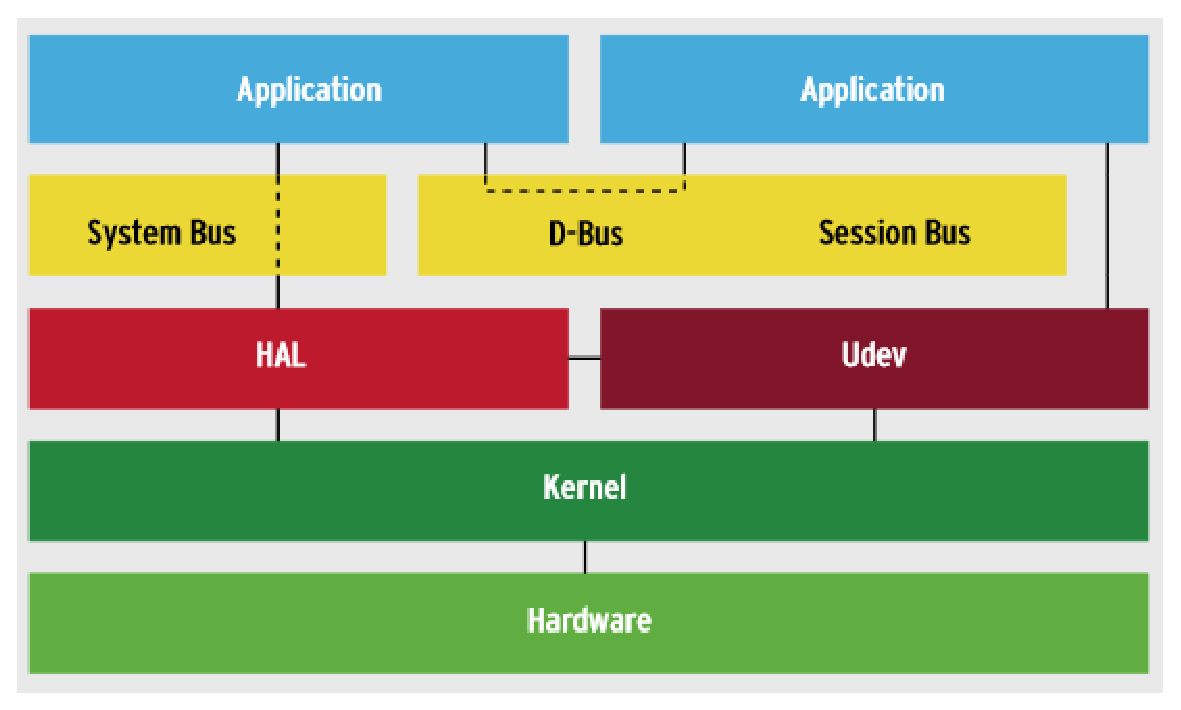
\includegraphics[height=5cm,
  angle=0]{./images/component_interaction.eps}}
  \caption{Scheme of Component Interactions}
  \label{fig:component_interaction_Linux}
\end{figure}


\subsection{udev + hotplug}
\label{sec:hotplug_udev}


% For dynamic device detection, previously, Linux used \verb!devfs! and
% \verb!hotplug! \footnote{\url{http://lwn.net/Articles/65197/}}. Here, the
% first SCSI disk detected is always /dev/sda, and then the second one is
% /dev/sdb (See below). 

\verb!udev! works at userspace mode (Sect.\ref{sec:udev_sysfs}). \verb!udev!
resolve many drawbacks of using \verb!devfs! in managing hardware devices. As
\verb!udev! only runs at userspace, it needs to daemon to provide the changes at
the system level. This is done by \verb!/sbin/hotplug! event handler.

The hotplug event handler is the process that detect the physical device and
notifies userspace that the kernel has discovered a new device. Then, the
userspace can try to load the module for that device, and do any other necessary
initialization so that users can use the device
\footnote{\url{http://lwn.net/Articles/123932/}}. This allows the device to be
detected automatically, i.e. Plug-n-Play feature in Linux. 

Different scripts were written for each device to function as a hotplug event
handler. These scripts have started since Linux kernel 2.3. From kernel 2.6,
instead of emitting the events for a limitted set of devices, with \verb!udev! being
used, hotplug event can be triggered for any device that has \verb!KObject!
registered in the \verb!sysfs! (Sect.\ref{sec:udev_sysfs}). 

\verb!udev! first use a single script \verb!/sbin/hotplug! as the hotplug event
handler.
\begin{verbatim}
### /sbin/hotplug script
DIR="/etc/hotplug.d"
for I in "${DIR}/$1/"*.hotplug "${DIR}/"default/*.hotplug ; do
        if [ -f $I ]; then
                test -x $I && $I $1 ;
        fi
done
exit 1
\end{verbatim}
It means that when a hotplug event is triggered, all programs in the
subdirectories will be notified. 

NOTE: If one program wants to be notified for all hotplug events, then it need
to be added (symlink) into \verb!/etc/hotplug.d/default/! directory. If one
programs cares about one type of bus event, they it is put into
\verb!/etc/hotplug.d/BUSNAME/! directory.
\textcolor{red}{The symlink for the program must end with .hotplug}. 

Example:
\begin{verbatim}
/etc/hotplug.d/
`-- default
    |-- 10-udev.hotplug -> ../../../sbin/udevsend
    |-- 20-hal.hotplug -> /usr/libexec/hal.hotplug
    `-- default.hotplug
\end{verbatim}
This example means that \verb!udevsend! is called first, and then by HAL, and
finally default linux-hotplug script.

\begin{framed}

With hotplug, the kernel needs to be compiled with \verb!CONFIG_HOTPLUG!. When a
device is plugged in, (e.g. ISA, USB, or PCI) bus controller signals the event
with an interrupt. In response to the interrupt, the kernel query the hardware
information and create a so-called KObject for each new device. Then
\verb!/sbin/hotplug! (\verb!/proc/sys/kernel/hotplug!) is evoked via the kernel
call to \verb!kset_hotplug! function (source: /lib/kobject.c). The device
information, located in, say
\begin{verbatim}
/devices/pci0001:01/0001:01:19.0/usb2/2-1/2-1:1.0 
\end{verbatim}
is passed to the program via DEVPATH variable. Other parameters: MAJOR, MINOR,
\verb!UDEV_EVENT!, SEQNUM, ACTION, etc. The kernel then makes this information
available at user-space via Sys-FS.

\end{framed}


Later one, major changes was added (udev 0.50 release), so that the
jobs in userspace is simpler. Since Linux kernel 2.6.11, \verb!/sbin/udevsend!
is the new kernel hotplug event handler.

In Ubuntu this is how it works
\footnote{\url{http://askubuntu.com/questions/28613/how-does-automated-hotplug-mounting-work}}
\begin{enumerate}
  \item The kernel detects and initialize the device (via \verb!dmesg!) and
  export the device information to userspace via the directory /sys/devices
  \item A \verb!uevent! signal is sent by the kernel to \verb!udev! daemon
  \item \verb!udev! daemon then gather the information and check the config
  files in \verb!/etc/dev/rules.d/! and \verb!/lib/udev/rules.d/! for rules
  about symlink to create in /dev folder. 
  
  \item \verb!udisks! daemon (with gvfs-gdu-volume-monitor) then can create the
  appropriate directory in /media folder and mount the device.
  \item nautilus then check the contents of the device, and open a new window if
  it is configured to do so. NOTE: nautilus also looks into /media/*/autorun.inf
  file for executable content.
   
\end{enumerate}

hotplug virtual memory and CPU:
\url{http://erny-rev.blogspot.com/2012/12/memory-and-cpu-hotplug-on-ubuntu-guests.html}

References:
\begin{enumerate}
  \item  \url{http://www.linux.com/news/hardware/peripherals/180950-udev}

  \item \url{http://lwn.net/Articles/123932/}
  
  \item
  \url{http://www.linuxfromscratch.org/pipermail/lfs-chat/2003-April/012639.html}
  
  \item \url{https://www.kernel.org/doc/local/hotplug-history.html}
  
  \item
  \url{http://www.kroah.com/linux/talks/ols_2003_udev_paper/Reprint-Kroah-Hartman-OLS2003.pdf}
  
  \item \url{http://www.lanana.org/docs/device-list/devices-2.6+.txt}
\end{enumerate}

\subsection{dbus}	
\label{sec:dbus}

\verb!dbus! is a system bus used for inter-process communication. 

\subsection{HAL}
\label{sec:HAL}

\verb!HAL! gets information from the \verb!udev! service, i.e. when a device is
inserted \verb!HAL! creates an XML representation for the device and then
notifies the corresponding Desktop application through \verb!dbus! and Nautilus
to open the device.

\section{GCC build}
\label{sec:gcc}

\subsection{gcc 4.7.x}
\label{sec:gcc-4.7.x-build}


It requires: (1) GMP (GNU Multi-Precision package) (gmp-devel), MPFR
(Portable Multi-Precision Floating-Point with correct rounding based on GMP)
(mpfr-devel) and MPC (Multiple-precision for complex number).
\begin{verbatim}
apt-get install libgmp-dev libmpfr-dev
\end{verbatim}

GCC 4.7.x comes with Ubuntu 12.04. It requires \verb!binutils! newer than the
one in Ubuntu 10.04, which is likely to cause the problem. At first, we need to build
\verb!binutil! from source, then build gcc 4.7 from source, and
\verb!DEB_BUILD_OPTIONS=nocheck!. IMPORTANT: Use chroot (man debootstrap) to
avoid any error to the system to happen. 

\url{http://askubuntu.com/questions/176914/is-it-possible-to-compile-gcc-4-7-1-on-ubuntu-10-04-manually}.


The script to install without root 
\begin{verbatim}
#!/bin/sh
# ***************************************************************************
# This script adapted from:
#    http://advogato.org/person/redi/diary/240.html
# For use in getting a standard gcc 4.7 for ATLAS stable 3.10 testing
#
# Assumes M4 is already installed; can get it from package manager on
# any Linux that I know of.
# ***************************************************************************
instd=/home/whaley/local/gcc4.7.0   # change this to your path
bldd=/home/whaley/TEST              # change to your build dir, /tmp OK
np=12                               # set this to your number of cores
# ------------------------------------------------------------
# Get and unpack the files, and stick them in common directory
# ------------------------------------------------------------
#cd ${bldd}
#mkdir GCC4.7.0
#cd GCC4.7.0
#wget http://www.netgull.com/gcc/releases/gcc-4.7.0/gcc-4.7.0.tar.bz2
#wget http://www.netgull.com/gcc/infrastructure/gmp-4.3.2.tar.bz2
#wget http://www.netgull.com/gcc/infrastructure/mpc-0.8.1.tar.gz
#wget http://www.netgull.com/gcc/infrastructure/mpfr-2.4.2.tar.bz2
#  ---------------------------------------------------------
#  Assuming we have all needed packages in current directory
#  ---------------------------------------------------------
bunzip2 -c gmp-4.3.2.tar.bz2 | tar xf -
bunzip2 -c mpfr-2.4.2.tar.bz2 | tar xf -
gunzip -c mpc-0.8.1.tar.gz | tar xf -
bunzip2 -c gcc-4.7.0.tar.bz2 | tar xf -
mv gmp-4.3.2 gcc-4.7.0/gmp
mv mpfr-2.4.2 gcc-4.7.0/mpfr
mv mpc-0.8.1 gcc-4.7.0/mpc
mkdir MyObj
cd MyObj
../gcc-4.7.0/configure --prefix=${instd} --enable-languages=c,fortran
make -j ${np}
make install
\end{verbatim}



\subsection{gcc 4.8.x}
\label{sec:gcc-4.8.x-build}


It requires: (1) GMP (GNU Multi-Precision package) (gmp-devel), MPFR
(Portable Multi-Precision Floating-Point with correct rounding based on GMP)
(mpfr-devel) and MPC (Multiple-precision for complex number).
\begin{verbatim}
apt-get install libgmp-dev libmpfr-dev
\end{verbatim}

If your Linux distro doesn't have them, download the source file and compile them
individually in the following order [NOTE: Use Modules to manage version -
Sect.\ref{sec:modules}]
\begin{verbatim}
http://gmplib.org/ (5.1.2)

http://www.mpfr.org/mpfr-current/ (3.x)

http://www.multiprecision.org/ (1.x) 
\end{verbatim}
Steps:
\url{http://stackoverflow.com/questions/9450394/how-to-install-gcc-from-scratch-with-gmp-mpfr-mpc-elf-without-shared-librari}

The libraries are installed to /usr/local/lib (by default), so make sure it's in
\verb!LD_LIBRARY_PATH!, before you compile gcc 4.8. You may get the error
\begin{verbatim}
gnu/stubs-32.h: No such file or directory
\end{verbatim}
then you need to install libstdc++-devel.i686.
\begin{verbatim}
yum install glibc-devel.i686
yum install libstdc++.i686
\end{verbatim}

NOTE: If you're using \verb!gcc 4.4.x!, then you may get
the error (check config.log) with \verb!-static-libstdc++! not recognized. This option means that
if the system supports both statically linking libstdc++ and dynamically linking
it, prefer statically linking it. Normally, the default is to dynamically link.
Only from GNU 4.5 this compiling option is supported. So open \verb!Makefile!
and remove it.
\begin{verbatim}
Libraries have been installed in:
   /packages/gcc/4.8.0/lib/../lib64

If you ever happen to want to link against installed libraries
in a given directory, LIBDIR, you must either use libtool, and
specify the full pathname of the library, or use the `-LLIBDIR'
flag during linking and do at least one of the following:
   - add LIBDIR to the `LD_LIBRARY_PATH' environment variable
     during execution
   - add LIBDIR to the `LD_RUN_PATH' environment variable
     during linking
   - use the `-Wl,-rpath -Wl,LIBDIR' linker flag
   - have your system administrator add LIBDIR to `/etc/ld.so.conf'
\end{verbatim}

After installing successfully GCC 4.8, you may get the error when running your
code compiled with new GCC
\footnote{\url{http://stackoverflow.com/questions/5216399/usr-lib-libstdc-so-6-version-glibcxx-3-4-15-not-found }}
\begin{verbatim}

\end{verbatim}
the reason is that you don't have the latest \verb!libstdc++.so.6.0.18!, look
for them in your gcc 4.8 source folder
{\small \begin{verbatim}
sudo cp x86_64-unknown-linux-gnu/libstdc++-v3/src/.libs/libstdc++.so.6.0.18 /usr/lib64/
\end{verbatim}}


Error FAQs: \url{http://gcc.gnu.org/wiki/FAQ#configure_suffix}

\subsection{-- compile gcc errors}

{\tiny
\begin{verbatim}
gcc/config/i386/linux-unwind.h: In function 'x86_fallback_frame_state':
gcc/config/i386/linux-unwind.h:138:17: error: field 'info' has incomplete type " 
\end{verbatim}
}

It's a well known issue between old gcc and newer versions of glibc at different
architectures.
As a temporary workaround it is proposed to patch gcc/config/i386/linux-unwind.h
or \verb!x86_64-unknown-linux-gnu/32/libgcc/md-unwind-support.h!

\begin{verbatim}
    {
      struct rt_sigframe {
       int sig;
-      struct siginfo *pinfo;
+      siginfo_t *pinfo;
       void *puc;
-      struct siginfo info;
+      siginfo_t info;
       struct ucontext uc;
      } *rt_ = context->cfa;
      /* The void * cast is necessary to avoid an aliasing warning.
\end{verbatim}
\url{http://pastebin.com/VkgE27Pd}


{\bf TROUBLE}
\begin{verbatim}
/usr/bin/ld: cannot find crti.o: No such file or directory
\end{verbatim}
or SOLUTION:
\begin{verbatim}
sudo ln -s /usr/lib/x86_64-linux-gnu/crti.o /usr/lib/crti.o
sudo ln -s /usr/lib/x86_64-linux-gnu/crtn.o /usr/lib/crtn.o
sudo ln -s /usr/lib/x86_64-linux-gnu/crt1.o /usr/lib/crt1.o
\end{verbatim}

SOLUTION: add
\begin{verbatim}
-B/usr/lib/x86_64-linux-gnu to the CFLAGS variable in your Makefile
\end{verbatim}
or add 
\begin{verbatim}
export LIBRARY_PATH=/usr/lib/x86_64-linux-gnu:$LIBRARY_PATH
\end{verbatim}
\url{http://askubuntu.com/questions/251978/cannot-find-crti-o-no-such-file-or-directory} 

% or SOLUTION:
% \begin{verbatim}
% sudo ln -s /usr/lib/x86_64-linux-gnu /usr/lib64
% \end{verbatim}
\url{http://stackoverflow.com/questions/6329887/compiling-problems-cannot-find-crt1-o}




\subsection{gcc 5.4}
\label{sec:gcc-5.4-build}

Fix:
\begin{verbatim}
../x86_64-unknown-linux-gnu/libgo/zstdpkglist.go: No such file or directory
\end{verbatim}
with
\begin{verbatim}
libgodir = ../../$(target_noncanonical)/libgo
\end{verbatim}



\section{Graphics}

\url{http://hybrid-graphics-linux.tuxfamily.org/index.php?title=Main_Page}

\url{http://wiki.openelec.tv/index.php?title=Configuring_a_Custom_xorg.conf}
\subsection{Intel X.org}

\verb!xf86-video-intel X.Org! driver
\begin{verbatim}
>> cat /etc/X11/xorg.conf.d/20-intel.conf
 
Section "Device"
Identifier "Intel Graphics"
Option "SwapbuffersWait" "true"
Option "AccelMethod" "sna"
Option "TearFree" "true"
EndSection
\end{verbatim}

\url{https://01.org/linuxgraphics/}
\url{http://wiki.gentoo.org/wiki/Intel}
\url{http://www.thinkwiki.org/wiki/Intel_HD_Graphics}
\url{http://elrepo.org/tiki/xorg-x11-drv-intel}

\url{http://www.x.org/wiki/IntelGraphicsDriver/}
\url{http://cgit.freedesktop.org/xorg/driver/xf86-video-intel/}

\url{https://wiki.archlinux.org/index.php/Intel_Graphics}

\url{https://wiki.freebsd.org/Intel_GPU}

\subsection{Nvidia driver}
\label{sec:Nvidia_driver}

\begin{verbatim}
apt-get remove nvidia-common nvidia-current
apt-get --purge remove nvidia-*
gedit /etc/modprobe.d/blacklist.conf
\end{verbatim}
and to the file
\begin{verbatim}
blacklist vga16fb
blacklist nouveau
blacklist rivafb
blacklist nvidiafb
blacklist rivatv
\end{verbatim}
then run
\begin{verbatim}
update-initramfs -u
\end{verbatim}
and reboot
\begin{verbatim}
sh NVIDIA.....run
\end{verbatim}
We need to use driver 295.20 and later to work with CUDA 4.1. 

Install CUDA toolkit (4.1 or latest) and SDK
\begin{verbatim}
sh nvidia...
sh gpucomputing...
\end{verbatim}

Install necessary packages to build the SDK
\begin{verbatim}
apt-get install libxi-dev libglut3-dev freeglut3-dev libxmu-dev -y
\end{verbatim}
NOTE: Ubuntu 12.04 doesn't have libglut3-dev; rather the closest matches are
\verb!freeglut3-dev!.

NOTE: Ubuntu, CUDA and gcc version
\begin{enumerate}
  \item Ubuntu 9.10 and 10.04 has gcc-4.4 by default
  \item Ubuntu 11.04 has gcc-4.5 by default
  \item CUDA 2.3/3.0 works with gcc 4.3 
  \item CUDA 3.2/4.0 works with gcc 4.4
  \item CUDA 4.1 works with gcc 4.5
\end{enumerate}
For Ubuntu 11.04 and CUDA 4.0
\begin{verbatim}
apt-get install gcc-4.4 g++-4.4
cd /usr/bin
ln -sf gcc-4.4 gcc
\end{verbatim}

Install Python, Pycuda, NumPy and Scipy: see Python book.

Install Infiniband (Chap.\ref{sec:Infiniband}).


Update NVIDIA Driver on all machines
\begin{verbatim}

pdsh -w cea[1-11],leak,cardiac -R ssh "cd /home/minhtuan/install_download;
   sh NVIDIA-Linux-x86_64-295.53.run -a -q -s"
\end{verbatim}

To look for more advanced options,
run\footnote{\url{http://us.download.nvidia.com/XFree86/Linux-x86/256.35/README/installdriver.html}}
\begin{verbatim}
sh NVIDIA-Linux-x86_64-295.53.run --advanced-options
\end{verbatim}

For NUMA systems, we may need some utilites
\begin{verbatim}
apt-get install libnuma1 numactl libnuma-dev -y 
\end{verbatim}

\subsection{Troubleshooting}

To remove locked files
\begin{verbatim}
rm /var/cache/apt/archives/lock; rm /var/lib/dpkg/lock
\end{verbatim}

To increase size of \verb!/tmp! 1MB problem
\begin{verbatim}
cp: failed to extend `/tmp/mkinitramfs': No space left on device

root@dhpr:/home/minhtuan# df
Filesystem                      1K-blocks       Used  Available Use% Mounted on
/dev/sda2                       467795128   14603508  429775148   4% /
udev                             16429924         12   16429912   1% /dev
tmpfs                             6575572        972    6574600   1% /run
none                                 5120          0       5120   0% /run/lock
none                             16438924          0   16438924   0% /run/shm
overflow                             1024       1024          0 100% /tmp
\end{verbatim}
This happens if you just run out of diskspace on the \verb!/root! partition. To
resolve the issue, you do either 
\begin{enumerate}
  \item Unmount 
\begin{verbatim}
umount /tmp
\end{verbatim}
and run the command
\begin{verbatim}
echo 'MINTMPKB=0' > /etc/default/mountoverflowtmp
\end{verbatim}
\url{http://unix.stackexchange.com/questions/60731/overflow-tmp-mounted-when-there-is-free-space-on}

  \item Open \verb!/etc/mtab!, look for the line something like
\begin{verbatim}
 overflow /tmp tmpfs rw,size=1048576,mode=1777 0 0
\end{verbatim}
Delete that line (or comment out), save and restart the computer.
\textcolor{red}{A better solution: keep the line, and remove the}
\verb!size=####!; this will allows the tmp directory to grow to half of the
available RAM, or \textcolor{red}{modify the size to 1/2 RAM and 1/2 of configured swap space}.

NOTE: Some distro now use \verb!tmpfs!, so you will see tmpfs, not \verb!/tmp!.


\end{enumerate}

\section{User account}
\label{sec:user_account}

In Linux-based O/S, \verb!root! is the user account with the highest privilege
(i.e. SuperUser). This account is created by default, and we cannot remove it.
In Ubuntu, by default, the password for \verb!root! account is locked, to avoid amateur user
from accessing this account. To be able to run any commands like \verb!root!
user, we need to put that user to a special group (Sect.\ref{sec:groups} and
Sect.\ref{sec:sudo}).

There are 2 types of users: those that are {\it distributed} to all machines,
and those that are {\it local} to the machine. By default, all users are local,
unless NIS is used (Sect.\ref{sec:NIS}).

\subsection{local user}

To manipulate user account for NIS, we use 

\subsection{-- create new user}

\textcolor{red}{create a new user}:  \verb!useradd!, \verb!adduser! or
  \verb!newusers!

useradd is native binary compiled with the system. But, adduser is a perl script
which uses useradd binary in back-end. adduser is more user friendly and
interactive than its back-end  useradd. There's no difference in features provided.
  
The newusers command is usefull when you have to add (or update) an entire list
of users. And it is very simple to use.
\begin{verbatim}
$>cat filewithusers

wolverine:passwd1::::/home/wolverine:/bin/bash

xavier:passwd2::::/home/profesorx:/bin/bash

storm:passwd3::::/home/preetystorm:/bin/bash

$> newusers filewithusers
\end{verbatim}
\url{http://linuxg.net/three-tools-for-creating-users-in-debian-based-distros-useradd-adduser-and-newusers/}

\subsection{-- remove user}

\textcolor{red}{remove an existing user}: \verb!userdel!, \verb!deluser!
  

\subsection{-- change user's GID or IID}

NOTE: When you change user's group or ID using the following commands, it
automatically update files/folders's attributes inside the \verb!$HOME! folder.
However, those outside need to be updated manually. You can issue the search
below
\begin{verbatim}
# find / -group 2000 -exec chgrp -h foo {} \;
# find / -user 1005 -exec chown -h foo {} \;
\end{verbatim}

\begin{itemize}
  
  \item assign a new UID to a user
  
\begin{verbatim}
# usermod -u 2005 <user-name>
\end{verbatim}

  \item assign new GID to a user
  
\begin{verbatim}
# groupmod -g 3000 <user-name>
\end{verbatim}

  \item \textcolor{red}{changing a user's group}:
  \verb!usermod! (recommend to use \verb!-aG! option)

Example:
\begin{verbatim}
## (i.e. remove a user from any existing group)
usermod -g users john

## allow more than one groups to be specified (the ones in /etc/group) 
usermod -G john,users,staff,websrv,whatever john

## only append a group to the current list of groups that a user is a member
usermod -aG <newgroup> <user>
\end{verbatim} 

  \item \textcolor{red}{add a group to a user} (manage /etc/group and
  /etc/gshadow):   \verb!gpasswd!
  
  Every group can have administrators, members and a password. The admin can
  use \verb!gpasswd! command with \verb!-A! option to define the
  administrator, \verb!-M! to define the members (or \verb!-a! to add a new
  user). \url{http://manpages.ubuntu.com/manpages/hardy/man1/gpasswd.1.html}
    
Example:
\begin{verbatim}
## add a new user
## gpasswd -a <user> <group>
## remove an existing user
## gpasswd -d <user> <group>

$> gpasswd -a john users 
$> gpasswd users -a john

$> sudo usermod -aG <group> $(whoami)

$> sudo usermod -aG <group> $USER
\end{verbatim}

  Group passwords are an inherent security problem since more than one
  person is permitted to know the password. However, groups are a useful
  tool for permitting co-operation between different users.

\end{itemize}. 

The useradd, userdel and usermod commands are lowlevel utilities which are there
for historical reasons, while \verb!adduser!/\verb!deluser! is the ones
recommended to use.
\url{http://askubuntu.com/questions/345974/what-is-the-difference-between-adduser-and-useradd}

To check which groups a user is belonging to
\begin{verbatim}
$> id -Gn

$> groups
\end{verbatim}

\subsection{sudo (sudoer)}
\label{sec:sudo}

The first user account created when you install the Linux-based O/S, e.g.
Ubuntu, is the user with the capability to run the command with root-level
privileges via the \verb!sudo <command>!. 

Whoever can run \verb!sudo! command is known as a \verb!sudoer!. 
NOTICE: There is a change from Ubuntu 11.10 (and earlier) to Ubuntu 12.04 (and
after). 

\begin{itemize}
  \item Ubuntu 11.10 and earlier: The users belong to the group \verb!admin! can
  do the \verb!sudo! command.
 
  \item Ubuntu 12.04 and later: The users should belong to the group \verb!sudo!
  instead.
\end{itemize}

There are 2 ways to put a user as a \verb!sudoer!. 
\begin{enumerate}
  \item modify the file \verb!/etc/groups!: and add a username after \verb!sudo! group
  
  
  This group is not special by itself, the reason it is special because the group's privilege is decided 
  inside the \verb!/etc/sudoers! file 
  
  
  
  \item modify the file \verb!/etc/sudoers! file (Sect.\ref{sec:etc/sudoers})
  

  \item or the addition of a configuration file to /etc/sudoers.d.
  
  The preferred way to do local configuration addition is to add a file to /etc/sudoers.d with the required configuration.
  Use visudo to at least verify these changes
  
\end{enumerate}

{\bf How to maintain user's environment settings with sudo command?}:
\url{https://wiki.archlinux.org/index.php/Sudo}
The recommended way of preserving environment variables is to append them to \verb!env_keep!. Example
the file \verb!/etc/sudoers.d/x2goserver! file
\begin{verbatim}
Defaults env_keep += "QT_GRAPHICSSYSTEM"
\end{verbatim}
For Ubuntu 14, you need to specify in separate lines as it returns the errors for multi-variable lines:
\begin{verbatim}
Defaults  env_keep += "http_proxy"
Defaults  env_keep += "https_proxy"
Defaults  env_keep += "HTTP_PROXY"
Defaults  env_keep += "HTTPS_PROXY"
\end{verbatim}

Configure to keep environment variable for a specific command only
\begin{verbatim}
Defaults!/bin/[your_command] env_keep += "http_proxy https_proxy"
\end{verbatim}
\url{https://stackoverflow.com/questions/8633461/how-to-keep-environment-variables-when-using-sudo}

Example: we want to enable a command - which requires sudo to run - to be able to run, by a regular user who does not have sudo privilege. 
The command \verb!etherwake! - to be run by \verb!mass! user! - requires root or \verb!sudo!. 
\begin{verbatim}
maas ALL= NOPASSWD: /usr/sbin/etherwake
\end{verbatim}
to the content of \verb!/etc/sudoers.d/99-maas-sudoers! file.


In either way, the users of this group needs to authorize the action, by retype
the password. The benefit of using \verb!sudo! to execute a command
\begin{itemize}
  \item by asking for the password, it adds one barrier before the execution of
  the command. It avoid any unexpected command to run.
  
  \item a log entry is kept in \verb!/var/log/auth.log!. If we mess up, we can
  always go back and see what command we run.
  
  \item prevent brute-force attack to \verb!root! account, as it is more
  difficult to know your account's name.
\end{itemize}
\url{https://help.ubuntu.com/community/RootSudo}

Some times, we don't want a particular user to be able to run any commands, but
just certain comamnds; or the user can run \verb!sudo! without typing the
password. This requires the admin to understand how to modify
\verb!/etc/sudoers! file and the files in \verb!/etc/sudoers.d/! folder
(Sect.\ref{sec:etc/sudoers}.


\textcolor{red}{Update sudo program}:  latest version 1.8.25 which uses file grammar version 46; and I/O plugin version 1.8.25
\begin{itemize}
  \item Ubuntu 14.04 has 1.8.9p5 by default - which uses file grammar version 43; and I/O plugin version 1.8.9p5
\end{itemize}
\url{https://www.sudo.ws/news.html}
If we upgrade, it may modify
\begin{verbatim}
/etc/pam.d/sudo

/etc/sudoers   
\end{verbatim}
files. 

\subsection{groups}
\label{sec:groups}

There are special groups:
\begin{itemize}
  \item \verb!adm!: this is different from \verb!admin! group 
  
  Group \verb!adm! is used for system monitoring tasks. Members of this group
  can read many log files in /var/log, and can use xconsole. Historically, /var/log
  was /usr/adm (and later /var/adm), thus the name of the group.
  \url{http://ubuntuforums.org/showthread.php?t=1318346} 
  
  \item \verb!admin! : this is deprecated since Ubuntu 12.04 LTS
  \url{https://bugs.launchpad.net/ubuntu/+source/policykit-1/+bug/893842} 
  
  Up until Ubuntu 11.10, the user created during installation belongs to
  \verb!admin! group, not \verb!sudo!, i.e. administrator access using the sudo
  tool (Sect.\ref{sec:sudo}) was granted via the admin Unix group. However,
  Debian is different.
  
  Conversely, on Debian the group enabled in /etc/sudoers is the \verb!sudo!
  group, and there is no \verb!admin! group. But the user created during
  installation is not put in that group, because Debian has the root account
  enabled by default; while it is not in Ubuntu.
  
  \item \verb!sudo!
  
  In Ubuntu 12.04, administrator access will be granted via the \verb!sudo!
  group. This makes Ubuntu more consistent with the upstream implementation
  and Debian. Administrators are added to the \verb!sudo! group, but the
  \verb!admin! group is still being supported for backward compatibility.
\end{itemize}




\subsection{/etc/sudoers file;  /etc/sudoers.d/ folder}
\label{sec:etc/sudoers}

The admin can controls which users can use \verb!sudo! and with which commands
by modifying \verb!/etc/sudoers! file or adding/modifying the files in
\verb!/etc/sudoers.d/! folder.

\begin{verbatim}
%sudo   ALL=(ALL:ALL) ALL

%admin   ALL=(ALL) ALL
\end{verbatim}
\label{sec:sudoers-file}

Another important information/setting is \verb!Default!

\begin{verbatim}
  // reset the environment setting at sudo
Default env_reset   


// as of Debian 1.7.2p1-1
// which read and parse any file inside the folder
//  that does not end with ~ or contain . (dot)
// NOTE: the files must be 0440 mode
#includedir /etc/sudoers.d
\end{verbatim}

IMPORTANT: \verb!visudo! command is the recommended way to update the file.
\begin{verbatim}
sudo visudo
\end{verbatim}
\label{sec:visudo}


Example: In some cases, you may want to remove the password prompt for your
account when using \verb!sudo! command. We need to be cautious when enabling
this feature, but we may need to use this when we want some other programs to
launch the \verb!sudo! command without password.

\begin{itemize}
  \item We modify \verb!/etc/sudoers! file (not directly opening the file but
  using \verb!sudo visudo! command)

Traditionally, visudo opens the /etc/sudoers file with the "vi" text editor.
Ubuntu, however, has configured visudo to use the "nano" text editor instead. To
change it back to \verb!vi!, run 
\begin{verbatim}
sudo update-alternatives --config editor
\end{verbatim}
or modify the environment variable
\begin{verbatim}
export EDITOR=/path/to/editor
\end{verbatim}

Example: Sect.\ref{sec:vim_variants}
\begin{verbatim}
 sudo update-alternatives --config editor
[sudo] password for tietronix:
There are 4 choices for the alternative editor (providing /usr/bin/editor).

  Selection    Path                Priority   Status
------------------------------------------------------------
* 0            /bin/nano            40        auto mode
  1            /bin/ed             -100       manual mode
  2            /bin/nano            40        manual mode
  3            /usr/bin/vim.basic   30        manual mode
  4            /usr/bin/vim.tiny    10        manual mode

Press enter to keep the current choice[*], or type selection number: 3
\end{verbatim}
\url{https://www.digitalocean.com/community/tutorials/how-to-edit-the-sudoers-file-on-ubuntu-and-centos}


  \item some packages may requires \verb!sudo! roles, so it can drop sudoers
  rule by creating a new file in the folder \verb!/etc/sudoers.d/!. Rule file
  names: not end in \verb!~! nor contains a \verb!.! character. 
  
IMPORTANT: The file \verb!/etc/sudoers! need to have the line (since Debian
1.7.2p1-1)
\begin{verbatim}
#includedir /etc/sudoers.d
\end{verbatim}
This enables \verb!sudo! to read and parse any files in the
\verb!/etc/sudoers.d! folder. LIMITATION: This requires at least 1 file in the
folder (and thus a \verb!README! file is there).

\end{itemize}

The content of the \verb!/etc/sudoers! file or
any files in the \verb!/etc/sudoers.d/! folder is composed of two types of
entries
\begin{enumerate}
  \item aliases (define variables)
  \item user specification (define who may run what)
\end{enumerate}
The grammar is described using EBNF (Extended Backus-Naur Form).

{\bf Aliases:} There are 4 kinds of aliases:
 \verb!Cmnd_Alias!, \verb!User_Alias, Runas_Alias!, or \verb!Host_Alias!. 
NOTE: The reserved word ALL is a built-in alias that always causes a match to
succeed. It can be used wherever any of the 4 aliases is expected.
The detailed rule is 
\begin{verbatim}
Alias ::= 'User_Alias'  User_Alias (':' User_Alias)* |
          'Runas_Alias' Runas_Alias (':' Runas_Alias)* |
          'Host_Alias'  Host_Alias (':' Host_Alias)* |
          'Cmnd_Alias'  Cmnd_Alias (':' Cmnd_Alias)*
 
User_Alias ::= NAME '=' User_List
 
Runas_Alias ::= NAME '=' Runas_List
 
Host_Alias ::= NAME '=' Host_List
 
Cmnd_Alias ::= NAME '=' Cmnd_List
 
NAME ::= [A-Z]([A-Z][0-9]_)*
\end{verbatim}
\url{http://www.sudo.ws/sudoers.man.html}

{\bf User specification}: determine which commands a user mayrun (and as what
user) on which hosts. The basic structure is
\begin{verbatim}
who where = (as_whom) what
\end{verbatim}
Detail rules
\begin{verbatim}
User_Spec ::= User_List Host_List '=' Cmnd_Spec_List \
              (':' Host_List '=' Cmnd_Spec_List)*

User_List ::= User |
              User ',' User_List
 
User ::= '!'* user name |
         '!'* #uid |
         '!'* %group |
         '!'* %#gid |
         '!'* +netgroup |
         '!'* %:nonunix_group |
         '!'* %:#nonunix_gid |
         '!'* User_Alias

Host_List ::= Host |
              Host ',' Host_List
 
Host ::= '!'* host name |
         '!'* ip_addr |
         '!'* network(/netmask)? |
         '!'* +netgroup |
         '!'* Host_Alias
                   
Cmnd_Spec_List ::= Cmnd_Spec |
                   Cmnd_Spec ',' Cmnd_Spec_List
 
Cmnd_Spec ::= Runas_Spec? SELinux_Spec? Solaris_Priv_Spec? Tag_Spec* Cmnd
 
Runas_Spec ::= '(' Runas_List? (':' Runas_List)? ')'
 
SELinux_Spec ::= ('ROLE=role' | 'TYPE=type')
 
Solaris_Priv_Spec ::= ('PRIVS=privset' | 'LIMITPRIVS=privset')
 
Tag_Spec ::= ('NOPASSWD:' | 'PASSWD:' | 'NOEXEC:' | 'EXEC:' |
              'SETENV:' | 'NOSETENV:' | 'LOG_INPUT:' | 'NOLOG_INPUT:' |
              'LOG_OUTPUT:' | 'NOLOG_OUTPUT:')
\end{verbatim}


\textcolor{red}{\bf Use exclamation (\!))}: (though it is rarely used due to
security) 

Example: for example, to match all users except for root one would use
\begin{verbatim}
ALL,!root
\end{verbatim}
If ALL is omitted, it would explicitly deny root but not match any other users. 

\textcolor{red}{\bf Put rules for groups (admin or sudo group)}: user
specification 

Example: \verb!/etc/sudoers! file
\begin{verbatim}
# Members of the admin group may gain root privileges
%admin ALL=(ALL) ALL

# Allow members of group sudo to execute any command
%sudo   ALL=(ALL:ALL) ALL
\end{verbatim}
NOTICE the difference: (ALL) vs. (ALL:ALL)
\begin{itemize}
  \item (ALL) : run the commands \verb!as any user!
  \item (ALL:ALL) : run the commands \verb!as any user! and \verb!as any group!
\end{itemize}
\url{http://askubuntu.com/questions/43317/what-is-the-difference-between-the-sudo-and-admin-group}


Example: user \verb!alan! can run any command as either \verb!root! or
\verb!bin!, optionally setting	the group to \verb!operator! or \verb!system!
\begin{verbatim}
alan	ALL = (root, bin : operator, system) ALL
\end{verbatim}

Example: allow user \verb!maas! to run \verb!sudo! on any node (ALL) with no
need to type password (NOPASSWD) on the commmand 
\verb!/usr/sbin/service maas-dhcpd restart! 

\begin{verbatim}
maas ALL= NOPASSWD: /usr/sbin/service maas-dhcpd restart
\end{verbatim}

\subsection{distributed user (NIS)}

When NIS is installed, pre-existing account, defined in \verb!/etc/passwd!
becomes local by default (on both master and slave machines).
\begin{verbatim}
/etc/passwd 
      entries for all active accounts.
/etc/group 
      entries for active groups
/etc/shadow
      entries for password of the accounts defined in /etc/passwd      
\end{verbatim}
The files (all residing at \verb!/etc! folder).

If we use NIS (Sect.\ref{sec:NIS}), on the master machine with NIS installed,
you can decide to
\begin{itemize}
  \item  use users defined in \verb!/etc/passwd! to be distributed users

  \item (RECOMMENDED) put the distributed users in a separte file, e.g. 
/etc/passwd.yp  and put local account in \verb!/etc/passwd! (or
/etc/passwd.local). If an entry is duplicated in two or more files, the entry
from the local file is used.

Similarly, we should use these files
\begin{enumerate}
  \item \verb!/etc/group.yp! : contains entries for distributed groups
  \item \verb!/etc/shadow.yp! : contains encrypted passwords
\end{enumerate}

\end{itemize}

IMPORTANT: We cannot directly create user account to /etc/passwd.yp,
/etc/group.yp, /etc/shadow.yp. What we can do is 
on the NIS master machine,  
\begin{itemize}
  \item modify directly the file /etc/passwd
  (or /etc/passwd.yp) file, add a new line for a new user 
  %(Sect.\ref{sec:user_account}).
\begin{verbatim}
minhtuan:x:2016:100::/home/minhtuan:/bin/bash
\end{verbatim}
NOTE: The third field is the user-ID (which should be larger than the minimum
value of MINUID given in /var/yp/Makefile, if you want the account to be
distributed). The fourth field is the groupd-ID (which should be larger than the
minimum value of MINGID given in /var/yp/Makefile, if you want the account to be
distributed). 

If this method is used, remember to create the home folder for the account in
\verb!/home/!. 
\begin{verbatim}
cd /home 
mkdir <userid>
chown <uid> <userid>
chgrp <group> <userid>
\end{verbatim}

  \item  use \verb!useradd! commands or \verb!newusers! commands to add the new
  user as local users; then we move the account information to the corresponding
  files (/etc/passwd.yp), and
delete them in /etc/passwd, etc.

   \item regenerate the database for the NIS:
   
Each time we add a new user or change the password for NIS, if the system is
Debian, we need to update the NIS
\begin{verbatim}
cd /var/yp
make
service portmap restart
/etc/init.d/nis restart
\end{verbatim}
and on the NIS Slave server, we run
\begin{verbatim} 
/usr/lib/yp/ypinit -s dhpr
/etc/init.d/nis restart
\end{verbatim} 
From Ubuntu 13.04, we need to run
\begin{verbatim}
service ypserv restart
\end{verbatim}

If the system is RedHat, we need to run
\begin{verbatim}
/etc/init.d/portmap start
/etc/init.d/yppasswdd start
/etc/init.d/ypserv start
\end{verbatim}

   
\end{itemize}


\begin{framed}

  The file /etc/passwd (or /etc/passwd.yp) contains username, the encrypted
  password, password expiration information, UID, GID, fullname, home-directory path, and login
shell. The structure is as follows
\begin{verbatim}
root:x:0:0:root:/root:/bin/bash
\end{verbatim}
'x' or '*' in the second column means the password is encrypted and saved in
/etc/shadow file.

The file /etc/shadow (or /etc/shadow.yp) contains username, the encrypted
password, days (last passowrd changed, until change allowed, \ldots) for the
users given in the file above. 
\end{framed}

The encrypted password is encrypted using some method that if we look at the
first 3 characters in the second field, e.g. \verb!$6$! is the method number 6
\begin{verbatim}
minhtuan:$6$NmVmAqm3$WA9vFg6.:15966:0:99999:7:::
\end{verbatim}
If you check \verb!man 3 crypt!, then you will see that \verb!$6$! is SHA-512bit
encryption method.


On servers, we need three daemons active: \verb!ypserv! (both Master and Slave
to receive queries from Clients) and \verb!ypbind! (run on every machines to
locate the valid server for the domain), and \verb!yppasswdd! (allow NIS server
to change user password on client's request). Check with 
\begin{verbatim}
// on server
rpcinfo -p localhost
\end{verbatim}
make sure you see three of them.

To create a new user, we may need to readjust GID and UID
\begin{verbatim}
usermod -g 100 user_name
usermod -u 2004 username
\end{verbatim}

To move users' password to the shadow file, and replace the password by an
asterisk or an 'x' in the /etc/passwd file, we call the command
\begin{verbatim}
;; create /etc/shadow from /etc/passwd
pwconv  
\end{verbatim}

\subsection{Manage User and Group (UUID and GUID)}
\label{sec:UUID_GUID}

While you're logging as the user you want to check, you type
\begin{verbatim}
> id

uid=0(root) gid=0(root) groups=0(root),1(daemon),2(bin),3(sys),4(adm),
 5(tty),6(disk),7(lp),1020(users)

\end{verbatim}
or
\begin{verbatim}
uid=131(minhtuan) gid=1020(users) groups=1020(users)
uid=516(aman) gid=1020(users) groups=1020(users)
\end{verbatim}
Each file on disk belong to an owner and a group. However, the actual names of
user and group is not recorded but the UID and GID. UIDs and GIDs are integers
that range from 0 to about 65,535. They are stored in the file /etc/passwd. 
\begin{verbatim}
;; a sample line
bduda:!:300:350:Ben Duda:/home/bduda:/bin/ksh
\end{verbatim}
the first field is username, third field is UID, fourth field is GID. More
information about GID can be extracted from /etc/group. E.g.: the group name
with GID=350 is 'security'.
\begin{verbatim}
$grep ":350:" /etc/group
security:!:350:bduda
\end{verbatim}

We can run \verb!istat! command on a file to check which UID and GID the file
belongs to.
\begin{verbatim}	
istat filename_to_check
\end{verbatim}

When you create the same username on different machines, the username may not
have the same UID and GID. The reason is that the UID and GID are automatically
assigned the next available number. One way to avoid this is by using NIS, by
storing all the account information on the same machine and the other machines
read this information (Sect.\ref{sec:NIS_NYS_NIS+}). Otherwise, if the
username is locally created, we need to manually set UID and GUID the same:
\burl{http://www.ibm.com/developerworks/aix/library/au-standardUID/index.html}

To check user name within a given UID range, e.g. from 100 to 200, we can
do
\begin{verbatim}
awk -F: '$3 >= 100 && $3 <= 200' /etc/passwd
\end{verbatim}
To check if a user exist
\begin{verbatim}
id this_username
\end{verbatim}
To check if a group exist
\begin{verbatim}
id -g this_group
\end{verbatim}

When you change UID of a username or GID of a group, remember that the files
belong to that UID and/or GUID are not automatically update to the new UID or
GUID. As a result, they belong to a UID and/or GID whose username or group are
unknown. These files are called unowned files. Before we want to change UID and
GID, remember to follow these steps first.
\begin{enumerate}
  \item Scan your system for unknown files:
  \begin{verbatim}
  ;; scan files with no user (skipping Network File System mounts)
  find / \( -fstype jfs -o -fstype jfs2 \) -nouser -print
  
  ;; scan files with no group
  find / \( -fstype jfs -o -fstype jfs2 \) -nogroup -print 
  \end{verbatim}
  or we can user Perl script which run faster than standard Unix command. The
  Perl tool \verb!find2perl! can turn a regular AIX command into perl script.
  \begin{verbatim}
find2perl / \( -fstype jfs -o -fstype jfs2 \) -nouser -print >  find_owner_script.pl
  
  
find2perl  / \( -fstype jfs -o -fstype jfs2 \) -nogroup -print > find_group_script.pl
  \end{verbatim}
  or 
  \begin{verbatim}
  find / \( -fstype jfs -o -fstype jfs2 \) -nouser -print > find_owner_script.txt
  
  find  / \( -fstype jfs -o -fstype jfs2 \) -nogroup -print > find_group_script.txt
  \end{verbatim}	
  
  \item Update the username/group: If you find them, you need to decide which
  username and group they should belong to and update properly. A rule of thumb
  is to look at the owner/group of the folder/directory. For simple cases with a
  few files we can do
  \begin{verbatim}
  chown this_user list_of_files_here
  chgrp this_group list_of_files_here
  \end{verbatim}
  A better solution is
  \begin{verbatim}
  
  \end{verbatim}
  
  \item It's better to use some centrallized user administration (e.g. NIS). 
\end{enumerate}

To change UID of a particular user, we call, suppose the user 'brian' change to
a new UID=204
\begin{verbatim}
chuser ID=204 brian
\end{verbatim}
However, there's a big problem: every file is associated with a username through
the UID, not the username itself. So, when you change the UID of that username,
the files' UID are not automatically updated and thus no longer belong to that
username. This is a daughting task. We first need to search all files belong to
that user, and then change to the new UID. 
\begin{verbatim}
;; search for files 

;; change
chown brian list_of_files_here
\end{verbatim}

To change a user to a new group, we call
\begin{verbatim}
chuser pgrp=new_group_name brian
\end{verbatim}

To change the GID of a group, e.g. new GID=5003, we do
\begin{verbatim}
chgroup "id=5003" this_group
\end{verbatim}
Again, the GID of the files are not updated automatically. To change to the new
GID, we do
\begin{verbatim}
;; search for files

;; change
chgrp this_group list_of_files
\end{verbatim}



References:
\begin{enumerate}
  \item \url{http://www.ibm.com/developerworks/aix/library/au-satuidgid/}
  \item
  \url{http://www.unix.com/shell-programming-scripting/118122-list-uids-between-100-200-a.html}
  \item \url{http://www.cyberciti.biz/faq/linux-check-existing-groups-users/}
\end{enumerate}

 
% \subsection{Distributed accounts}



\subsection{Strong-Password check}

We open \verb!/etc/pam.d/passwd! and include

\begin{verbatim}
password   required     pam_cracklib.so retry=3 minlen=8 difok=3
password  required pam_unix.so nullok use_authtok md5 shadow use_first_pass \
           remember=12
\end{verbatim}
We may need to install the library
\begin{verbatim}
apt-get install libpam-cracklib
\end{verbatim}

The minimum number of characters in the password is defined in \verb!minlen!.
However, the real minimum characters can be less than this due to ``credits''
given to non-lowercase-alphabets given in the password string, e.g using number,
upper case or non-alphanumeric characters. The maximum credit given for
lower-case, upper-case, numeric, and non-alphanumeric are given below
\begin{verbatim}
lcredit=0 ucredit=1 dcredit=1 ocredit=2
\end{verbatim}
You can adjust the value and add to the line above as well.

NOTE: The maximum number of password it can store is 400; so any value greater
than 400 means 400. The old passwords are stored in
\verb!/etc/security/opasswd!. Make sure you set it the proper 
\begin{verbatim}
touch /etc/security/opasswd
chown root:root /etc/security/opasswd
chmod 600 /etc/security/opasswd
\end{verbatim}
You can use this to enhance the security, by avoiding users from reusing their
previous passwords untill after a certain number of times.




\url{http://www.techrepublic.com/article/enforce-strong-passwords-with-pam-passwdqc/}

\url{http://www.deer-run.com/~hal/sysadmin/pam_cracklib.html}


\subsection{File attributes (ownership): Files/Folders permission
(user/group/others)}

A file/folder can belong to 3 types of owners: user/group/others, each with
different permission, listed on the first column of the \verb!ls -l! command.

The most important columns are the first (contains the format
\verb!tuuugggooo!), the third (user name), and the fourth (group name).

Example:  
\begin{verbatim}
drwxr-xr-x 3 nana writers 90
-rw-r-xrw- 1 nana writers 8817 
drwrr-srwx 3 tom  root    292
\end{verbatim}

{\bf EXPLAIN}: \verb!tuuugggooo!
\begin{enumerate}
  \item  The first character refers to file attribute which means
  
$t$ can be 
\begin{verbatim}
d = directory
- = regular file
l = symbolic link
s = UNix domain socket
p = named pipe
c = character device file
b = block device file
\end{verbatim}

  \item The next 9 characters show the permission (enabled/disabled) for 3 types
  of owners, first triple characters for user, next triple characters for group and
the last triple characters for others (i.e. everyone else).

For each group (u, g, or $o$), the first is
enabled get \verb!r! = read permision, the second character get \verb!w!=write
permission, and the last  character can get \verb!x!=execute permission or
\verb!s!=suid is  enabled so that file/folder can be executed with root
permissions by all users. 

\begin{verbatim}
-   = no permission for that feature
w   = write allowed
r   = read allowed
x   = execution allowed
\end{verbatim}
Any position in the triple can get \verb!-!, i.e. no permission. 
 
\end{enumerate}

To look for files with suid permision, we do
\begin{verbatim}
find / -perm +4000
\end{verbatim}

To set \verb!rwsrwxrwx! we do
\begin{verbatim}
chmod 4777
\end{verbatim}

To \ldots from {\bf o}thers
\begin{verbatim}
 //remove all permission from all level of subfolders
chmod o-wrx  MyFolder -R

  //add excution this folder level 
chmod o+x    MyFolder 
\end{verbatim}


\section{Memory RAM}

A typical desktop PC uses Unbuffered DIMM (UDIMM). 


For server, a better option is Registered DIMM (RDIMM). Here, we can have 3
DIMMs per channel (DPC), yet it limits the speed to 1066 MHz. To run RDIMM at
1600 MHz, we can only use 2 DPC. RDIMM add a register, to buffer address and
command signals. 


A newer technology, Load-Reduced DIMM (LRDIMM) that supports higher memory
bandwidth and capacity. It allows higher capacity memory to runs at 3 DPC. The
main change is that registers are replaced by an Isolation Memory Buffer
(iMB) component. iMB can buffer command, address, and data signals.  


IMPORTANT: We cannot mix different DIMM technology on the same machine. 


The latest technology for these DIMMs is DDR3. 

\begin{enumerate}
  \item \url{http://www.micron.com/products/dram-modules}
  \item
  \url{http://www.supermicro.com/support/resources/memory/X9_DP_memory_config_socket_R.pdf}
  
  \item
  \url{http://www.anandtech.com/Show/Index/6068?cPage=3&all=False&sort=0&page=2&slug=lrdimms-rdimms-supermicros-latest-twin}
\end{enumerate}
\section{Name Service Switch (nsswitch.conf)}

Various functions in the C library (libc) need to be configured to work in the
local environment using /etc/passwd. In early times, many nameservices need to
hack into the C library to use. When other nameservices become popular, e.g.
NIS, DNS, a separate file needs to be used, allowing users to add new services
without adding them to the GNU C library. This allows the C library image
smaller. The names of all the services are written in the file
/etc/nsswitch.conf. 
\begin{enumerate}
  \item aliases: mail aliases
  \item ethers : ethernet
  \item group : group of users
  \item hosts : host names
  \item networks : network names
  \item passwd : user passwd
  \item shadow : shadow user passwd
\end{enumerate}

Each line is an entry for the service consisting the
database name in the first field, a semicolon, and a list of possible source
database mechanism 
\begin{verbatim}
passwd:     files ldap
shadow:     files
group:      files ldap

hosts:      dns nis files

ethers:     files nis
netmasks:   files nis
networks:   files nis
protocols:  files nis
rpc:        files nis
services:   files nis

automount:  files
aliases:    files
\end{verbatim}



\url{http://www.gnu.org/software/libc/manual/html_node/Name-Service-Switch.html} 


\section{Samba}
\label{sec:Samba}

Samba is a protocol on Windows like NFS (Sect.\ref{sec:NFS}) in Linux. 

\section{SSH}
\label{sec:SSH}
\label{sec:ssh}

SSH, which is an acronym for Secure SHell, was designed and created to provide
the capability to access a shell on a remote machine (running Linux/Unix). This
is better than using \verb!telnet! program (Sect.\ref{sec:telnet}).

Nowadays, SSH can do more than the original purpose
\begin{enumerate}
  \item (original) encrypt the session:
  
  encryptionfrom 512 bit on up to as high as 32768 bits and includes ciphers
  like AES (Advanced Encryption Scheme), Triple DES, Blowfish, CAST128 or
  Arcfour). NOTE: the higher the bits, the longer it will take to generate and
  use keys as well as the longer it will take to pass data over the connection. 
  
  \item better authentication facilities:
   
  \item secure file transfer, 
  \item X session forwarding, 
  \item port forwarding
  \item etc.
\end{enumerate}
\url{https://support.suso.com/supki/SSH_Tutorial_for_Linux}

\subsection{Dropbear SSH server/client}
\lavel{sec:Dropbear}

Dropbear is POSIX-based and is a relatively small SSH server and client, e.g.
useful for embedded type Linux systems.




\subsection{OpenSSH}
\label{sec:OpenSSH}

\begin{verbatim}
// openssh-7.6p1 
./configure --prefix=/packages/openssh/7.6
            --with-ssl-dir=/packages/openssl/1.0.2/ 
\end{verbatim}

\subsection{X11 forwarding (-X, -Y)}
\label{sec:X11-forwarding}

\begin{verbatim}
 -X      Enables X11 forwarding.  This can also be specified on a per-host
             basis in a configuration file.
         X11 forwarding is subjected to X11 SECURITY

-Y      Enables trusted X11 forwarding.  Trusted X11 forwardings are not
             subjected to the X11 SECURITY extension controls.
\end{verbatim}

NOTE: Users with X11 forwarding, i.e. \verb!-X! option, has the ability to
bypass file permissions on the remote host (for the user's X authorization
database) can access the local X11 display through the forwarded connection.
Because of that, X11 forwarding is subjected to X11 SECURITY extension
restrictions by default. If we trust the remote machine, we can use \verb!-Y!.

When using \verb!-X!, we can combine with the following options
on SSH client configuration file (Sect.\ref{sec:ssh_config})

\begin{itemize}
  \item \verb!ForwardX11Trusted! directive:
  
  \item \verb!ForwardX11! directive (yes, no (default)):
  
  If 'yes', it's equivalent to using \verb!-X! option 
  
  \item \verb!ForwardX11Timeout! directive: 
\end{itemize}


\subsection{ssh\_config (ssh client configuration file)}
\label{sec:ssh_config}

\begin{verbatim}
~/.ssh/config

/etc/ssh/ssh_config
\end{verbatim}

The \verb!ssh_config! is the ssh client configuration
file, that you modify to affect \verb!ssh!'s command-line option at user-level
and system-wide level. NOTE: You may configure at different location in the
file; however, for each parameter, the first obtained value will be used. 

\begin{enumerate}
  \item affect X11 forwarding - Sect.\ref{sec:X11-forwarding}
\end{enumerate}


\subsection{sshd\_config (ssh server configuration file)}
\label{sec:sshd_config}

The \verb!sshd_config! is the ssh daemon (or ssh server process) configuration
file, that you modify to
\begin{enumerate}
  \item change the SSH server port
  
  \item 
\end{enumerate}


\subsection{Port}

Default port is 22
\begin{verbatim}
Port 2222
\end{verbatim}
Modify \verb!/etc/sh/sshd_config! file

\subsection{Display login banner}

The content of the banner is in
\begin{verbatim}
/etc/issue.net 
\end{verbatim}

and put
\begin{verbatim}
Banner /etc/issue.net 
\end{verbatim}
Modify \verb!/etc/sh/sshd_config! file


\subsection{Restart}

\begin{verbatim}
sudo /etc/init.d/ssh restart
\end{verbatim}


\subsection{Time-out issue}

To avoid time-out connection, we use \verb!-o ServerAliveInterval=20! (in sec)
on the client-side
\begin{verbatim}
ssh -Y  minhtuan@199.26.254.42 -o ServerAliveInterval=20
\end{verbatim}
You can also set it as the default setting in \verb!/etc/ssh_config!.
\begin{verbatim}
ServerAliveInterval 20
\end{verbatim}

To avoid time-out connection, if you have \verb!root! access on the server-side,
you can modify the file \verb!/etc/sshd_config! and add
\begin{verbatim}
ClientAliveInterval 60
\end{verbatim}

\subsection{Password-less SSH connection}
\label{sec:passwordless-ssh}

Private/public key is a secured way to connect to remote machine. What if you
have different remote machines, that you just don't want to retype the password
to the private key every time. A good way is to set-up a private
key, and use \verb!ssh-add! to prompt users for the private key. 

Make sure to copy the public key (Sect.\ref{sec:public-private-key}) to all
your remote machines. Then, on your local machine, type (this is for SSH)
\begin{verbatim}
ssh-add
// prompt for password to private key
ssh-agent bash

// now you're free to connect to all these remote hosts without retyping the
// password
\end{verbatim}

If you use SSH2, then you need to use
\begin{verbatim}
ssh-add2
ssh-agent2 bash
\end{verbatim}



Password-less SSH connection allows you to register the machine A (SSH client)
to another machine B (SSH server) so that next time you login from the machine A,
the SSH server doesn't ask you for password. This saves times if you know that
only you can use the SSH client machine. Example: in case you have your own
laptop, i.e. the credentials for any connection from this laptop is supposed to
be from you only.

To do so, you need to use a public/private keypair generated by
\verb!ssh-keygen!. You keep the private key and share the public key to the SSH
server. There are three options
\begin{enumerate}
  \item RSA : the only method that is an encryption algorithm
  
  There are 2 versions: RSA1 (use in ssh1), and RSA (use in ssh2)
  
  \item DSA (Digital Signature Algorithm): digital signing and verifying, not
  for encryption and work with ssh2 only.
  
  \item ECDSA (Elliptic Curve implementation of DSA) : digital signing, but also
  provide the same security level as RSA with a smaller key and a lighter
  calculation workload-wise. 
\end{enumerate}
RSA should work with all SSH protocol. DSA requires SSH2 protocol, which is
quite common. ECDS support is newer.

{\bf For regular user}: Generate key pair (DSA uses SSH2 version which requires
all machines to support SSH2 protocol)
\begin{verbatim}
ssh-keygen -t dsa -b 1024

//to use 2048-bit
(umask 077 ; openssl dsaparam -genkey 2048 | openssl dsa -out ~/.ssh/id_dsa)
ssh-keygen -y -f ~/.ssh/id_dsa > ~/.ssh/id_dsa.pub
\end{verbatim}
By default, the private key is in \verb!~/.ssh/id_dsa! and the public key in
\verb!~/.ssh/id_dsa.pub!. We need to use a trick to enable 2048-bit DSA
\footnote{\url{https://digitalelf.net/2014/02/using-2048-bit-dsa-keys-with-openssh/}}

Copy the public key to the SSH server which store the list of public keys of the
machines that register with the server in \verb!~/.ssh/authorized_keys!.
\begin{verbatim}
cat .ssh/id_dsa.pub | ssh host 'cat >> ~/.ssh/authorized_keys'
\end{verbatim}
or using RSA (SSH1 version) 
\begin{verbatim}
ssh-keygen -t rsa
cat ~/.ssh/id_rsa.pub >> ~/.ssh/authorized_keys
scp -r ~/.ssh  hduser@10.10.10.106:~/
\end{verbatim}

You can instead use the command \verb!ssh-copy-id!.

\textcolor{red}{IMPORTANT}: 
Due to different SSH versions on servers, 
we need to set permissions on .ssh directory and \verb!authorized_keys! file.
\begin{verbatim}
# on target SSH server machine
chmod 700 .ssh; chmod 640 .ssh/authorized_keys

\end{verbatim}

{\bf For root user}: first and formorst, do not enable the root account + do not
set a password for the root account. So, we login to the remote machine under
root using public key authentication, not with a password. The reason is that
\footnote{\url{https://lists.debian.org/debian-security/2002/06/msg00418.html}}
if the client is infected, and you try to login to a remote machine with
'root' using the root password, the typed-in password is then logged, and if
this password is happed to be used on any other server, the attacker will have
access to those servers (you can have a different root password for different
servers; but this is not widely happen in practice). However, using keys, the
real password is unknown even if the client is infected. Logging in as root
using key  makes things like "scp" and other non-interactive programs possible
over SSH.

By doing this, you no longer need the password.

You may get the error
\begin{verbatim}
bad owner or permissions on .ssh/config 
\end{verbatim}
and the solution is 
\begin{verbatim}
chmod 600 ~/.ssh/config
\end{verbatim}

\subsection{Error message}

To check for error message, we use \verb!-v! option or \verb!-vv! option or
\verb!-vvv! (more detailed message) when connecting to the server.

\subsection{Public key authentication}
\label{sec:public-private-key}

Public key authentication is an alternative method than using password. You
generate a private key and public key. You keep the private key on your
local machine, and put the public key on the remote machine on which you want to
connect to. This allows the remote host 'A' to identify the machine that want to
connect to 'A'. 

To generate the key pair, on your local machine run
\begin{verbatim}
// SSH2 (more secured, but only works if both the local and remote
//      has SSH2 installed)
ssh-keygen -t dsa

// SSH
ssh-keygen -t rsa1
\end{verbatim}
You tell where to save the key pair (public/private) and what is the password to
get access to the private key. If you press enter, the default setting is used
(file \verb!.ssh/id_dsa! (for private key) and \verb!.ssh/id_dsa.pub! (for
public key) and no password to protect private key). It's strongly recommended
to use the password.
% jafri lab

Now, you want to copy the public key to your remote host
\begin{verbatim}
cat ~/.ssh/id_dsa.pub | ssh user@hostname "cat - >> ~/.ssh/authorized_keys"

// or
ssh user@hostname "echo `cat ~/.ssh/id_dsa.pub` >> ~/.ssh/authorized_keys"

// or
ssh-copy-id -i ~/.ssh/id_dsa.pub "-p 2222 user@server"
\end{verbatim}


\subsection{Passwordless SSH}

Sect.\ref{sec:passwordless-ssh}.

\subsection{pty}
\label{sec:pty}

Pseudo-terminal interfaces: A pair of virtual character devices (master + slave)
that provide a bidirectional communication channel. Pseudo-terminals are used by
SSH, RLOGIN, TELNET, etc. 

Two porpular pseudo-terminal APIS: BSD and System V. Linux provides both a
BSD-style (deprecated since kernel 2.6.4) and System V-style terminals (aka Unix
98 pseudo-terminals).

A master clone device is /dev/ptmx. When a process opens /dev/ptmx, it gets a
file descriptor for a pseudo-terminal master (PTM). A pseudo-terminal slave
(PTS) is created in /dev/pts/ directory. 

Linux kernel imposes a limit on the number of available Unix 98
pseudo-terminals. In kernels up to 2.6.3, this limit is defined in
\verb!CONFIG_UNIX98_PTYS! at kernel compilation time, i.e. if we want to
increase, set the new value for this variable, and recompile the kernel. Since
kernels 2.6.4, this limit can be dynamically adjusted by modifying the file
/proc/sys/kernel/pty/max. The number of pseudo-terminals are currently in use
can be read in the file /proc/sys/kernel/pty/nr.


\subsection{Security enhancements}

\url{http://www.la-samhna.de/library/brutessh.html#1}

\subsection{SSH tunneling}
\label{sec:SSH_tunneling}

One widely usage of SSH is to create a secured connection via a remote terminal
connection. Another use is SSH client acting as a SOCKS proxy; then you can
configure your applications on the client machine (e.g. the web browser) to use
the SOCKS proxy. Thus, any traffic over the network for that application is
forwarded through the SSH connection. This is known as {\bf SSH tunneling}.
The traffic enter the SOCK proxy and SSH client forward to the server through
SSH connection. It's encrypted too, but SSH tunnel doesn't offer all the benefit
of VPN (Sect.\ref{sec:VPN}).

Example: create a SOCK proxy at port 9999 at your local system
\begin{verbatim}
// ssh -D <port> -C user@host

ssh -D 9999 -C tom@localhost
\end{verbatim}
Then you can configure your web-browser (manual proxy configuration) to direct
all traffic to go through 
\begin{verbatim}
SOCKS Host = localhost       Port = 9999
(SOCKS v5)

No proxy for: localhost, 127.0.0.1
\end{verbatim}






\subsection{Troubleshooting}

\textcolor{red}{Error}:
\begin{verbatim}
Permission denied, please try again
\end{verbatim}

{\bf One possible reason } is that we miss the information of the underlying
shell, i.e. last field is not there
\begin{verbatim}
tmhoangt:x:1002:1003::/data/tmhoangt:
\end{verbatim}
FIX:
\begin{verbatim}
tmhoangt:x:1002:1003::/data/tmhoangt:/bin/bash
\end{verbatim}

{\bf Another possible reason is that the user is not in the list of accepted
ssh connection}, check  \verb!/etc/ssh/sshd_config!, and see what groups are
allowed to make ssh connection
\begin{verbatim}
AllowGroups sshusers
\end{verbatim}
FIX: Go to \verb!/etc/group! and check what users are in that group
\begin{verbatim}
sshusers:x:1001:tmhoangt
\end{verbatim}


\subsection{sshfs}
\label{sec:sshfs}

{\bf sshfs} is an easy way to mount remote filesystem using ssh
(Sect.\ref{sec:ssh}) and FUSE. Other options:
Sect.\ref{sec:mount-remote-filesystem}.

\url{http://www.saltycrane.com/blog/2010/04/notes-sshfs-ubuntu/}

{\bf Extreme fast sshfs} with these options
\begin{verbatim}
-o Ciphers=arcfour -o Compression=no


NOTE:
 'arcfour' cipher which is the fastest encryption method (and not very safe but
we don't care since it's a trusted network)

  disable the built-in compression SSH uses by default
\end{verbatim}
	 

{\bf Option 1}:
\begin{verbatim}
$sshfs root@10.232.139.234:/mnt/files /var/www/remote_files \
 -o IdentityFile=/path/to/my_ssh_keyfile \
 -o ServerAliveInterval=60 -o allow_other


NOTE: 
root is the ssh username
10.232.139.234 is the remote host
/mnt/files is the remote path
/var/www/remote_files is the local path
/path/to/my_ssh_keyfile is the ssh keyfile
The ServerAliveInterval option will keep your connection from timing out.
The allow_other option allows other users to access the filesystem
\end{verbatim}


{\bf Option 2}: put into /etc/fstab file
\begin{verbatim}
sshfs#root@10.232.139.234:/mnt/files /var/www/remote_files fuse
 allow_other,IdentityFile=/path/to/my_ssh_keyfile,ServerAliveInterval=60 0 0

\end{verbatim}




\section{SSL (OpenSSL)}
\label{sec:SSL}
\label{sec:OpenSSL}

Check version
\begin{verbatim}
 openssl version
\end{verbatim}

Version information is stored in
\begin{verbatim}
OPENSSL_VERSION_NUMBER = 0x0090819f 
   in /usr/include/openssl/opensslv.h
   (version = 0.9.8y)
\end{verbatim}

There are different versions:
\begin{itemize}
  \item 1.0.2n 
\end{itemize}

To BUILD (use shared = build .so files):
\begin{verbatim}
// openssl-1.0.2n
./config --prefix=/packages/openssl/1.0.2/ 
         --openssldir=/packages/openssl/1.0.2
         shared

./configure --prefix=/usr --with-ssl-dir=/usr/local/ssl --with-tcp-wrappers

//NOTE:
--with-openssl-includes=/usr/local/include and
--with-openssl-libraries=/usr/local/lib

\end{verbatim}

\subsection{error with user-installed SSL in Ubuntu}

{\tiny
\begin{verbatim}
libcrypto.so.1.0.0: no version information available
\end{verbatim}
}
\url{https://askubuntu.com/questions/830466/libcrypto-so-1-0-0-no-version-information-available-required-by-ssh}

The reason is that the Ubuntu version of OpenSSL has some additional patches
installed that are not included if you get your version of OpenSSL from elsewhere. 
Specifically, symbols exported by the library have version information
associated with them in \verb!Ubuntu OpenSSL! but not standard OpenSSL (at least
in versions prior to 1.1.0).

You get the "no version information available" warning if you run an Ubuntu
supplied application that is expecting the library to have versioned symbols,
but the library version you actually pick-up is a non-Ubuntu version that
doesn't have those versioned symbols. It will work (usually), but it will
complain about it.

The other problem sign is this:
\begin{verbatim}
OpenSSL 1.0.2g  1 Mar 2016 (Library: OpenSSL 1.0.1k 8 Jan 2015)
\end{verbatim}

This tells you that the OpenSSL command line app is 1.0.2g, but it is linking
against the 1.0.1k library. This is likely to cause crashes - normally the
command line app and the library should use matched versions.

The OpenSSL 1.0.2g  1 Mar 2016 bit of the version is what standard Ubuntu
OpenSSL will report. The OpenSSL 1.0.1k 8 Jan 2015 bit is coming from some
non-Ubuntu version of OpenSSL.

To resolve your problem you need to figure out where the non-Ubuntu OpenSSL is
and remove it from your library path.


\section{SysLinux}
\label{sec:syslinux}

Syslinux is a collection of different lightweight boot loaders. NOTE: Grub is a
single (heavy-weight) boot loader (Sect.\ref{sec:GRUB}).

Syslinux uses \verb!extlinux! to boot ext2, ext3, ext4 and BTRFS filesystem.
Support for NTFS has been started
\footnote{\url{http://www.sarducd.it/forum/english-forum/re-sardu-2-0-5-rc-4-multiple-installer-qemu-ntfs-t894.html}}


Since syslinux 4.0, \verb!extlinux! is merged into syslinux project.

To replace GRUB2 with syslinux as the bootloader, 
\begin{verbatim}
==> If you want to use syslinux as your bootloader
==> edit /boot/syslinux/syslinux.cfg and run
==> # /usr/sbin/syslinux-install_update -i -a -m
==> to install it.
\end{verbatim}
To automate the process of writing the MBR and installing relevant files to
\verb!/boot/syslinux/!. 

IMPORTANT: If the machine has a RAID array, then the \verb!--raid! flag should
be used.



\section{Portmap and inet.d}
\label{sec:portmap}

\subsection{Portmap}

RPC Portmapper is a server that convert RPC program number into TCP/IP protocol
port numbers using \verb!rpcbind! protocol. This will allows two RPC programs,
not using TCP/IP protocol, can communicate to each other. In Linux, it's name is
{\bf portmap} which is a dynamic port assignment daemon for RPC services, i.e.
keeps a list of what services are running and on what ports.
This must be installed on both client and server.
\begin{verbatim}
apt-get install portmap
\end{verbatim}
NOTE: \textcolor{red}{Since Ubuntu 11.10}, \verb!portmap! is no longer
available, it's replaced by \verb!rpcbind!, even though the package name to
install is the same.

With the daemon running, other machines can use the list (service-port) to see
which service/port is available to use. Example of RPC services are NIS and NFS. 
Also, we need to make sure SSH daemon is working on every machine
\begin{verbatim}
apt-get install openssh-server openssh-client
\end{verbatim}



For security issue, you should not make it accessible outside a trusted LAN.


In Ubuntu 10.04 and earlier, to check if you have a securable portmapper, type
\begin{verbatim}
strings /sbin/portmap | grep hosts
\end{verbatim}
If you see something like this
\begin{verbatim}
# strings /sbin/portmap | grep hosts.
/etc/hosts.allow
/etc/hosts.deny
@(#) hosts_ctl.c 1.4 94/12/28 17:42:27
@(#) hosts_access.c 1.21 97/02/12 02:13:22
#
\end{verbatim}
then the system is secured. Otherwise, you do the following 
\begin{enumerate}
  \item Add to /etc/hosts.deny
  \begin{verbatim}
  ;; to deny access to everyone
  portmap:: ALL
  \end{verbatim}
  save (which take affects immediately) and run
  \begin{verbatim}
  rpcinfo -p
  \end{verbatim}
  You no longer see \verb!portmapper!. But we don't want it to close for
  everyone. Thus, we edit the file
  /etc/hosts.allow\footnote{\url{http://nfs.sourceforge.net/nfs-howto/ar01s06.html}}
  \begin{verbatim}
  ;; to tell that all machines in the subnet 192.168.0.0 with
  ;; subnet mask 255.255.255.0 should have access to it
  portmap: 192.168.0.0/255.255.255.0
  \end{verbatim}
  NOTE: To check network mask, we use \verb!ifconfig! (Look for MASK:). To check
  network address, we use \verb!netstat -rn! (first column). 
  \textcolor{red}{It's important to use IP address only, not hostname in these
  files; and machines in your cluster should use static IPs.}
  
  
\end{enumerate}

Finally, we install NFS (Sect.\ref{sec:NFS})

\subsection{inetd.conf in Ubuntu}

In Linux, there's a program known as Internet ``superserver'' that listen on
ports and invoke the proper programs in response to connections. So, a
connection from a machine can be accepted or rejected based on
\verb!/etc/hosts.allow! and \verb!/etc/hosts.deny!, as well as other features
related to connections. The deamon that we're talking about is \verb!inetd!, a
service used by some service to listen on specific ports.

\begin{verbatim}
apt-get install openbsd_inetd 
\end{verbatim}
As these daemons are mainly run by root that a regular user never use or
configure, Ubuntu has the policy of not opening any port on default install.
So, \verb!inetd! is not installed by default. Then Ubuntu use a more powerful
choice \verb!/etc/xinetd.conf! (the eXtended inet) rather than inetd.conf. Other
options are: rlinetd, ucspi-tcp, etc. In Mac OS X 10.4, it uses \verb!launchd!.
This is becoming more popular when a single machine is widely used
to dedicate to a single task, e.g. an HTTP server is configured to just run
httpd, and no other ports opened. 

\begin{verbatim}
apt-get install xinetd
\end{verbatim}

However, it's also not installed by default. To install, we need to
install
\begin{verbatim}
apt-cache search inet-superserver
openbsd-inetd - The OpenBSD Internet Superserver
xinetd - replacement for inetd with many enhancements
inetutils-inetd - internet super server
rlinetd - gruesomely over-featured inetd replacement
\end{verbatim}

Later, more and more server daemons are designed to run securely as stand-alone
programs, rather than being invoked by xinetd. So, in recent Ubuntu, we don't
need xinetd at all. 

\subsection{Portmap and RPC}
\label{sec:portmap_RPC}

Remote procedural call (RPC) is a protocol for inter-process communication. This
allows one program (a client) to cause a subroutine/procedure to be executed in
another address space (the server), e.g. in a remote machine without knowing in
detail how the two machines connect to each other (Sect.\ref{sec:RPC}).

On the server machine (remote machine), {\bf portmapper} is the service (in
Linux O/S, they are \verb!portmap! or recently, \verb!rpcbind! daemon) that run
as a daemon that supply client programs with information about server programs.
Both programs use the well-known port 111.

Clients contact server programs by sending messages to the port numbers or
universal addresses of remote processes. A remote process registers itself to
the portmapper.
\begin{itemize}
  \item \verb!portmap! (support rpcbind protocol version 1, 2) returns port
  number of server program to convert RPC program number to TCP/IP (or UDP/IP) port numbers.

  \item \verb!rpcbind! (support rpcbind protocol version 1, 2,3,4) returns
  universal addresses, which is a text string (defined by RFC 3530) representing the
  transport dependent address. Rpcbind has more features, like IPv6 and NFSv4
  support.
  
The following are examples of universal addresses for port 1024 (port 1024 = port 0x400):
\begin{verbatim}
    9.1.1.1.4.0
    ::FFFF:9.1.1.1.1.4.0
    2001:0DB8::10:1:1:1.4.0
\end{verbatim}  

In HP-UX 11.00, portmap is replaced by rpcbind (completely transient to NFS
services). In Arch Linux (2009), portmap is replaced by rpcbind, i.e. modify
/etc/rc.conf and changes
\begin{verbatim}
portmap --> rpcbind
nfslock --> nfs-common
nfsd    --> nfs-server
\end{verbatim}
Fedora 12 and RHL6 dropped portmap and replaced it by rpcbind. 
The extended configuration options can be found in /etc/conf.d/nfs-common
and /etc/conf.d/nfs-server. 

From Ubuntu 11.10, {\bf portmap} is replaced by {\bf rpcbind}. 
  
\end{itemize}

E.g.: access to /etc/passwd is carried out via \verb!getpwuid()! system call.
When a RPC server starts, it register with portmap daemon the following information
(which port it's listening to, which RPC program numbers it serves).

\verb!rpcinfo! make an RPC call to the RPC server and reports the status of the
server. To probe the portmap service (default:
local host), we call
\begin{verbatim}
rpcinfo -p
\end{verbatim}
which display a list of registered RPC program to portmap.
%rpcinfo -p -a <IP_machine>



\section{Port/Firewall}


To test which ports are being used, we call
\begin{verbatim}
netstat -tlunp
\end{verbatim}

\section{License server}

License server is required to run IDL, MatLab, PGI Fortran. We may need to call
\begin{verbatim}
mkdir /usr/tmp
! or 
ln -s /tmp /usr/tmp
\end{verbatim}

Each license (for one vendor) is handled by a running (daemon) process, known as
{\it vendor daemon}. This vendor daemon keeps track of how many licenses are checked
out. The daemon process runs on the server, and talks to the client programs via
TCP/IP or UDP/IP sockets. 

The licensing information about a program is stored in a file, known as license
file (default names can be license.dat or license.lic). The location of this
file is specified in the environment variable
\begin{enumerate}
  \item \verb!MLM_LICENSE_FILE!: the same feature like \verb!LM_LICENSE_FILE!, yet
  is specific to MATLAB vendor daemon, {\bf MLM}. It means that it is used to
  set to the location of MATLAB-specific license file, if \verb!LM_LICENSE_FILE! has
  not been set.
  \item \verb!LM_LICENSE_FILE!: is used to set to the location of license
  file, used by FLEXlm. 
\end{enumerate}

The content of the license file can be, e.g. for MATLAB
\begin{verbatim}
# BEGIN--------------BEGIN--------------BEGIN                                                                                                    
# MathWorks license passcode file.
# LicenseNo: 539556   HostID: 001F2904143F
#
# R2012b
#
SERVER cardiac 001F2904143F 27000
USE_SERVER
VENDOR MLM
INCREMENT MATLAB MLM 28 01-jan-0000 1 4EE1C27A4082A81B5B4D \
        VENDOR_STRING=vi=0:at=200:ae=1:lu=200:lo=CN:ei=993314: \
        DUP_GROUP=UH asset_info=539556 ISSUED=10-Oct-2012 \
        NOTICE=product=MATLAB SN=539556
INCREMENT Optimization_Toolbox MLM 28 01-jan-0000 1 \
        8E41D29A01C18B668A2A \
        VENDOR_STRING=vi=0:at=200:ae=1:lu=200:lo=CN:ei=993314: \
        DUP_GROUP=UH asset_info=539556 ISSUED=10-Oct-2012 \
        NOTICE="product=Optimization Toolbox" SN=539556
INCREMENT Signal_Toolbox MLM 28 01-jan-0000 1 BEB142FAA2D3CD38071F \
        VENDOR_STRING=vi=0:at=200:ae=1:lu=200:lo=CN:ei=993314: \
        DUP_GROUP=UH asset_info=539556 ISSUED=10-Oct-2012 \
        NOTICE="product=Signal Processing Toolbox" SN=539556
INCREMENT Statistics_Toolbox MLM 28 01-jan-0000 1 \
        AE01D2BA15A02334325F \
        VENDOR_STRING=vi=0:at=200:ae=1:lu=200:lo=CN:ei=993314: \
        DUP_GROUP=UH asset_info=539556 ISSUED=10-Oct-2012 \
        NOTICE="product=Statistics Toolbox" SN=539556
# END-----------------END-----------------END
\end{verbatim}

\begin{enumerate}
  \item \verb!SERVER!: without this line, it means the license is node-locked,
  otherwise it's a floating license, and then you can run the client programs
  from other machines.
  \item \verb!VENDOR!: the name of the vendor licensing daemon 
\end{enumerate}



\subsection{MatLab}

\begin{verbatim}
/usr/local/MATLAB/R2012b/etc/glnxa64/lmgrd -c 
   /usr/local/MATLAB/license.lic
\end{verbatim}
Not using this
\begin{verbatim}
/usr/local/MATLAB/R2012b/etc/glnxa64/lmgrd -c 
   /usr/local/MATLAB/R2012b/licenses/network.lic
\end{verbatim}


On the server
\begin{verbatim}
%%export MLM_LICENSE_FILE=/usr/local/MATLAB/R2012b/licenses/network.lic
export MLM_LICENSE_FILE=/usr/local/MATLAB/license.lic
\end{verbatim}
On the client, suppose 'cardiac' is the name of the server
\begin{verbatim}
export MLM_LICENSE_FILE=27000@cardiac
\end{verbatim}
with 27000 is the port that MLM is
running\footnote{\url{http://www.mathworks.com/support/solutions/en/data/1-1A4TV/index.html?solution=1-1A4TV}}.

To enable autostart of the license manager, we can use the boot script in the
MATLAB 'etc' folder. The script name can be either  flexnet.boot.linux,
rc.lm.linux, rc.lm.glnx86, or rc.lm.glnxa64
\footnote{\url{http://www.mathworks.com/support/solutions/en/data/1-1AP76/index.html?solution=1-1AP76}}.
\begin{enumerate}
  \item Create the link
  \begin{verbatim}
ln -s $MATLAB/etc/lmboot /etc/lmboot_TMW
ln -s $MATLAB/etc/lmdown /etc/lmdown_TMW
  \end{verbatim}
  
  \item Copy the boot script to /etc/init.d/, we can rename it to lmgrd.matlab
  \item Change the permission
  \begin{verbatim}
  chmod 755 /etc/init.d/lmgrd.matlab
  \end{verbatim}
  
  \item Modify the script, like this
  \begin{verbatim}
if [ -f /etc/lmboot_TMW ]; then
   /etc/lmboot_TMW -u username && echo 'MATLAB_lmgrd'
fi
  \end{verbatim}
  with \verb!username! is the name of user (should not be root).
  
  \item Run 
  \begin{verbatim}
  update-rc.d /etc/init.d/lmgrd.matlab defaults
  \end{verbatim}
  Or we just link to level 3
  \begin{verbatim}
cd /etc/rc3.d
ln -s ../init.d/lmgrd S17lmgrd
  \end{verbatim}
  
\end{enumerate}


\subsection{PGI Fortran}

To run the license server for PGI, we do
\begin{verbatim}
/opt/pgi/linux86-64/2012/bin/lmgrd.rc start
\end{verbatim}
which invoke \verb!lmgrd! to do  proper works.

\subsection{Troubleshooting}

\subsubsection{lmgrd}

Running lmgrd on Ubuntu machine may give us the error
\begin{verbatim}
./lmgrd: No such file or directory
\end{verbatim}
while the file is there. The reason is that FLEXnet lmgrd license manager daemon
is not officially supported on Ubuntu, but is supported on any completely Linux
Standard Base (LSB) compatible operating system. So, it needs to have \verb!lsb!
package installed.
\begin{verbatim}
apt-get install lsb
\end{verbatim}

Another way to check if what's wrong with the binary file, we use \verb!strace!
or \verb!ltrace! utility
\begin{verbatim}
strace ./lmgrd
\end{verbatim}

To check if \verb!lmgrd! is running, run
\begin{verbatim}
ps -ax | grep 'lmgrd'
\end{verbatim}

However, it's not recommended to run it as root user. With 'username' is a
regular user
\begin{verbatim}
su username -c `umask 022; /path/lmgrd -c /path/license.dat -l /path/log'
\end{verbatim}

To run it automatically at boot, we add this line to /etc/rc.local
\begin{verbatim}
/opt/pgi/linux86-64/2011/bin/lmgrd.rc start
\end{verbatim}

\subsubsection{License Manager Error -98}

\begin{verbatim}
License checkout failed.
License Manager Error -97
License Manager cannot start.

http://www.mathworks.com/support/solutions/en/data/1-184BQ/?s_cid=pl_LME97_R2008a
\end{verbatim}
This can happen when the file /var/tmp/lockMLM exists. Try to remove the file,
shutdown the license mamanger and then rerun the license manager.
\begin{verbatim}
sudo rm /var/tmp/lockMLM
$MATLAB_DIR/etc/lmdown
su daemon
/etc/init.d/lmgrd.matlab start
\end{verbatim}
As we cannot run with root user, we need to specify a username to run, e.g.
daemon.
\begin{verbatim}
$MATLAB_DIR/etc/lmstart -u daemon
\end{verbatim}

\section{Update Packages}

The file /etc/apt/sources.list contains package information. It contains pairs
of lines which tell where to find the binary (pre-compiled) packages (deb) and
source packages (deb-src)
\begin{verbatim}
deb http://host/debian distribution section1 section2 section3
deb-src http://host/debian distribution section1 section2 section3
\end{verbatim}
It can accept different types of sources:  http, ftp, file (local files, e.g., a
directory containing a mounted ISO9660 filesystem) and ssh.

NOTE: After modifying the file, run 
\begin{verbatim}
apt-get update
\end{verbatim}

\subsection{Download packages}

You can download packages only using
\begin{verbatim}
apt-get install packagenames --download-only
\end{verbatim}
or if the packages has been installed, we need
\begin{verbatim}
apt-get install --force-reinstall true <package1> <package2> --download-only
\end{verbatim}

We can do
\begin{verbatim}
#save the list of installed packages
dpkg --get-selections > packages.txt
#clear all selected packages
dpkg --clear-selections
apt-get clean
#download the packages (say pidgin)
apt-get install --reinstall -d --print-uris --yes pidgin
#restore the list of installed packages
dpkg --set-selections < packages
\end{verbatim}

To download a package with all dependencies, we use \verb!gdebi!
\begin{verbatim}
apt-get install gdebi-core
\end{verbatim}
To list all dependencies we use (say 'gfortran' package)
\begin{verbatim}
apt-cache depends gfortran
\end{verbatim}
Then, to let dpkg handles the dependencies, we just do
\begin{verbatim}
dpkg -i /path/to/*.deb
\end{verbatim}


\subsection{Sources is local folder}

We create a folder which contains the list of .deb files
\begin{verbatim}
mkdir /root/debs
\end{verbatim}
This folder can be mounted. Download the binary packages to local folder
(default is /var/cache/apt/archives)
\begin{verbatim}
apt-get install <packages> --download-only
\end{verbatim}

Install a package
\begin{verbatim}
dpkg -i /path/to/deb/file.deb
\end{verbatim}
but it don'ts look for dependencies. To install a package, from command-line
with all dependencies, you can use \verb!gdebi-core! or gdebi. A similar tool
\verb!apt-get! only looks for dependencies from http or ftp sources. 

\subsection{Sources is CD-ROM}

Put the DVD into the CD-ROM
\begin{verbatim}
apt-cdrom add
\end{verbatim}
or you can specify the CD-ROM mount point, which is good to use remote CD-ROM
\begin{verbatim}
apt-cdrom -d directory add 
\end{verbatim}

To mount the CD-ROM from a remote machine, we do
\begin{enumerate}
  \item on the remote machines: mount the CD-ROM on the remote machine to
  /mnt/cd-rom
  \begin{verbatim}
  mkdir /mnt/cdrom
  mount /dev/sr0 /mnt/cdrom/ -o loop
  ;; or (if you have GNOME)
  mount --bind "/media/Ubuntu 10.04.4 LTS amd64"/ /mnt/cdrom/
  \end{verbatim}
  
  \item on every local machines, we do (suppose the name of remote machine is
  'cardiac')
  \begin{verbatim}
  mkdir /mnt/cdrom
  sshfs cardiac:/mnt/cdrom /mnt/cdrom/
  \end{verbatim}
  We can use \verb!pdsh! to mount all at once.
  
  \item then, run on these local machines
  \begin{verbatim}
  ln -s /mnt/cdrom /media/apt
  sudo apt-cdrom add -m
  \end{verbatim} 
\end{enumerate}

\section{Superblock}

A file is a collection data (e.g. music, picture, book, etc.) stored on disk. A
directory is a group of files. There are 2 types of directory: root director
(denoted by /), and subdirectories (under root).

To help organizing files and directories, there are different file system types:
ext2, ext3, NFS. To find out, we can do
\begin{verbatim}
cat /proc/mounts
\end{verbatim}
A collection of files and directories used by the Linux OS is called Linux
{\bf file system}: /, /usr, /var, /tmp. 

A disk is organized in groups of so-called blocks. Most blocks stores user data
(files). Some blocks store file system's metadata. {\bf Metadata} describes the
structure of the file system. Most common metadata are {\bf superblocks}, inode
and directories. Superblocks keep critical information: file system type (ext2
or ext3), size (how big??), status (working or not), information about other
metadata structures. If this information is lost, you're in trouble.

To keep the system from corruption, Linux keeps multiple redundant copies of the
superblock in every file system. To retrieve the location of the backup
superblock on /dev/sda, we can do
\begin{verbatim}
dumpe2fs /dev/sda | grep -i superblock
\end{verbatim}
Output looks like
\begin{verbatim}
Primary superblock at 0, Group descriptors at 1-1
Backup superblock at 32768, Group descriptors at 32769-32769
Backup superblock at 98304, Group descriptors at 98305-98305
Backup superblock at 163840, Group descriptors at 163841-163841
Backup superblock at 229376, Group descriptors at 229377-229377
Backup superblock at 294912, Group descriptors at 294913-294913
\end{verbatim}
An alternative command is 
\begin{verbatim}
mke2fs -n /dev/sda
\end{verbatim}

To repair the file system using the alternative-superblock, first we make the
backup of the disk first
\begin{verbatim}
dd if=/dev/sda of=/disk2/backup-sda.img
\end{verbatim}
then, we pick up one of the backuped superblock and call
\begin{verbatim}
e2fsck -f -b 32768 /dev/sda

;; or for the RAID array
e2fsck -f -b 32768 /dev/md1
\end{verbatim}

\subsection{RAID Superblock}

A RAID array is also a special device. Linux RAID reserves a bit of space
(called superblock) on each component device, which hold the metadata about the
RAID device, and allow correct assembly of the
array\footnote{\url{https://raid.wiki.kernel.org/index.php/Superblock}}.
Depending on the metadata being used, RAID has 3 distinct variant superblocks:
pre-0.9,  version-0.90 and version-1.x.

Superblock version-0.90 is the default during RAID array creation on most
distributions. However, it has several limitations that limits its uses on large
array, i.e. limit to 28 devices, and each device is limited to 2TB. The
superblock is 4KB  in size, and is written into a 64K aligned block that starts
at least 64K and less than 128K from the end of the device.
Linux kernel 2.4 to 2.6.28 can only recognize superblock version-0.90.
Boot-loader LILO can boot from superblock version-0.90 only; yet not a
limitation with GRUB2\footnote{\url{https://raid.wiki.kernel.org/index.php/RAID_superblock_formats}}.


Superblock version-1 is well supported, but not the default. It can supports
384+ devices, and 64-bit sector lengths. There are three variants, which differ
mainly where the superblock is stored (1.0: at the end of the device (at least
8K, but less than 12K from the end), 1.1: at the beginning of the device (stop
you from directly mounting, without going through \verb!md! tool), and 1.2: at
4K from the beginning of the device (useful if you make RAID array on the whole
device, which doesn't need partition tables, MBR)). The total size is 256bytes,
+2bytes per device in the RAID array.

The kernel automounter cannot mount any of the version 1.x superblocks. As a
result, we cannot use UUID in the /etc/fstab. We thus can add this to
/etc/rc.d/rc.sysinit
\begin{verbatim}
 # Start any MD RAID arrays that haven't been started yet
[ -f /etc/mdadm.conf -a -x /sbin/mdadm ] && /sbin/mdadm -As --auto=yes --run
\end{verbatim}

References:
\begin{enumerate}
  \item
  \url{http://www.cyberciti.biz/tips/understanding-unixlinux-filesystem-superblock.html}
\end{enumerate}
  
\section{RAID}
\label{sec:RAID}

{\bf RAID} stands for Redundant Array of Indepenent Disks. It's not a backup
solution, but to improve (1) reliability, and (2) disk I/O (performance) with
two basic strategies:
\begin{enumerate}
  \item mirrored RAID: the files are written at least twice, once to each hard
  drive (good for constant backup). It requires at least 2 harddrives. This is
  to improved reliability, as if one disk dies, the whole data can be recovered.
  But only the image of the data at the last time point.
  
  
  
  \item striped RAID: the files are split and placed segments on different hard
  drive (speed up file access). This is to improve data I/O speed (i.e.
  parallel I/O). However, if one drive fail, your data is not completed, and
  thus you're totally screwed.
\end{enumerate}
It's better to have a mirrored and striped RAID. This requires at least 3
harddrives, so when one disk is failled,  a new one can put in its place to
maintain the stripe. Information about different configurations is given in
Sect.\ref{sec:RAID_configurations}, while the technique to implement that is
given in Sect.\ref{sec:RAID_software-hardware}.

\subsection{RAID: minimum disk + disk redundancy}

\begin{verbatim}
Name      Minimum disk       #Disk-redundancy         

RAID0     2                  0
RAID1     2                  1
RAID5     3                  1
RAID6     4                  2
RAID10    4
(10 = 1+0)    2 for one mirror (RAID 1)
              2 for one copy   (RAID 0)
              1 for O/S (must not on the array)                  
\end{verbatim}
\url{http://www.smbitjournal.com/2012/11/choosing-a-raid-level-by-drive-count/}

\subsection{RAID configurations (standard RAID, hybrid RAID)}
\label{sec:RAID_configurations}

Depending on the configuration, there are 10 different levels of standard RAID:
RAID0 \ldots RAID9.
\begin{itemize}
  \item RAID0 (data striping on two or more hardrive becomes one logical
  unit):  minimum 2 disks, excellent performance (blocks are striped), no
  redundancy (no mirror, no parity). Not safe for critical systems. 
  \item RAID1 (data mirroring, i.e. data are written at the same time to
  different harddrives):
  minimum 2 disks, good performance (no striping, no parity), excellent
  redundancy (blocks are mirrored). Data are save with minimum 2 copies, each on every harddrive.
  
  \item RAID4 (data striping with dedicated parity) 
  
  \item RAID5 (data striping with distributed parity, i.e. P-stripe): minimum 3
  disks, good performance (blocks are striped), good redundancy (with distributed parity).
  The array is not destroyed by a single drive failure, as the lost part can be
  calculated from distributed parity.
  When one drive fails, we need to replace and rebuild the data.
  
  Methods for parity distribution can be: left-symmetric, right-symmetric,
  left-assymmetric, right-assymmetric. 
  
  \item RAID6 (data striping with double distributed parity, i.e. P-stripe and
  Q-stripe): a more flexible choise than RAID5, with 2 harddrive failure
  tolerance using double distributed parity i.e. Q-stripe contains Galois
  Field (GF) sum of data.
  Yet the performance can be lower than RAID5, due to more complicated management. 
  
\end{itemize}

In addition to standard RAID, we can also have hybrid (nested) RAID
\begin{enumerate}
  \item RAID0+1: striped set in a mirrored set (minumum 4 hardrives: A+B as
  RAID0, C+D as RAID0 with C+D is the mirror of A+B).
  The machine continue to work if one or more drive in the same mirror set failed.
  
  \item RAID10: mirrored set in a striped set (minimum 4 harddrives: A and B
  are mirrored, C and D are mirrored, and the results are striped).
  It's better than RAID0+1 (as long as no mirror loses all of its drives).
  
  \item RAID50:
  \item RAID51:
\end{enumerate}
Non-standard RAID is given in
\url{http://en.wikipedia.org/wiki/Non-standard_RAID_levels}. 

\begin{framed}
RAID parity is an error protection scheme to provide fault tolerance in a given
set of data, so that when one or more of the drive fail, the whole data can be
reconstructed on the spare disk. Most use simple XOR parity; RAID6 uses two
separate parity check based on addition and multiplication in a particular
Galois Field, i.e. Reed-Solomon code (an error-correcting algorithm based on
Galois Algebra).
\end{framed}

RAID is also a technique to enlarge the capacity, by combining many physical
drives (/dev/sda, /dev/sdb, etc.) or partitions (/dev/sda1, /dev/sda2,
/dev/sdb1, etc.) into a single logical disk (\verb!/dev/md0!, \verb!/dev/md1!)
on a single machine. We can also combines RAID array from different machines
into a single logical disk, using multiple layers like LVM, but it can be
complicated to manage (Sect.\ref{sec:LVM_RAID}). 

References:
\begin{enumerate}
  \item \url{http://www.ufsexplorer.com/inf_raid.php}
\end{enumerate}

\subsection{Software vs. Hardware RAID}
\label{sec:RAID_software-hardware}

To map multiple physical disks into a single logical disk, we need a {\bf disk array controller}. The
disk array controller is often confused as disk controller, as they provide very
different functionality. A disk array controller has 2 interfaces: a back-end
interface to talk to the physical disks, i.e. providing protocols like ATA,
SATA, SCSI, FC \footnote{FC = fibre channel which is often used at enterprise
level (supercomputer), \url{http://en.wikipedia.org/wiki/Fibre_Channel}}; a
front-end interface interact with the computer's host adapters and provide data
via a communication protocol (e.g. ATA, SATA, SCSI, FC, Infiniband). In the case
of RAID (Sect.\ref{sec:RAID_configurations}), the disk array controller is the
RAID controller.


The RAID controller is the device intermediate between the servers and the data
storage. The RAID controller can be internal to the server (e.g. a chip or
card), or external (e.g. a network-attached storage NAS). Here is the
classification
\begin{verbatim}
         Host-Based   	         	|	External Controller-Based
    Internal   |	External   	    |     	All External
SATA 	|SCSI    |	JBOD Enclosures |	iSCSI 	|   Fibre Channel (FC)
\end{verbatim}

\begin{itemize}
  \item Internal host-based RAID can be SATA or SCSI. SATA-based products:
  Escalade 9000 SATA RAID (AMCC 3ware), four-port SRCS14L controller (Intel).
  
  \item The external host-based RAID is not really RAID. It is ``just a bunch of disks''
(JBOD). The two JBOD products are DF2000J (LSI Logic) and FS4100 Fibre to SATA
JBOD (Adaptec)
\footnote{\url{http://www.enterprisestorageforum.com/hardware/features/article.php/11184_3351361_2/Storage-Basics-Choosing-a-RAID-Controller.htm}}
  
  \item In External controller-based RAID: FC is the dominant back-end
  (companies: Network Appliance, Digi-Data with STORM family of RAID
  controllers)
\end{itemize}

Here we focus on internal host-based RAID controller which can be hardware-based
or software-based, i.e.  {\bf hardware RAID} or {\bf software RAID}.
\begin{enumerate}
  \item hardware RAID is expensive as you need to buy hardware RAID controllers,
  and unconvenient as the disk may not work with a different RAID card. A
  cheaper solution is called {\it fakeRAID}. It also use a hardware device, but
  is cheaper. It is simply a standard disk controller chip with special firmware
  and drivers, i.e. it doesn't have a RAID controller chip.  Adaptec call it
  {\it host RAID}. It use the daemon {\bf dmraid} (Sect.\ref{sec:fakeRAID}).

Early times of hardware RAID (before 1997) requires disk with SCSI interface,
which is expensive. Advantages of SCSI are independent data transfer, hot-swapping, upto
15 devices on one bus.	The first ATA RAID controller was introduced as a
PCI-expansion card. Even though it's cheaper, most lack a dedicated buffer or
high-performance XOR hardware for parity calculation. 	


  \item software RAID:  Software RAID is only available since Linux kernel 2.4
  and is managed by {\bf mdadm} daemon (md = multiple devices,
  adm=administrator).
\end{enumerate}
 

\textcolor{red}{Why software RAID?}: 
In overall, software RAID is better for RAID0 and RAID1, Table.\ref{tab:RAID}.
Only software RAID allows us to mix different drives and sizes (yet the capacity
of the RAID disk is the size of the partition/drive of the smallest capacity).
Besides, recovering from disk failure is easier with software RAID, as we
can swap the harddrive to another machine and read the data transparently, i.e. no vendor
lock or no secret block-level optimization at the disk
header\footnote{\url{http://superuser.com/questions/83923/can-a-mirrored-raid-1-disk-be-plugged-into-another-system-to-be-read}}.


\textcolor{red}{Why hardware RAID + software RAID?}: Sometimes, we need to do
both software and hardware, e.g. for a database server, 4 mirror pairs, 2 on
each hardwared RAID controller, and use software RAID0 to put it all together.

\begin{table}[hbt]
\begin{center}
\caption{Hardware vs. Software RAID}
%\begin{tabular}{ p{2cm} |c|c}
\begin{tabular}{ c |c|c} 
  \hline
Feature	 & Software & Hardware \\ 
  \hline\hline
Cost & Cheap & Expensive	\\
Can act as a back-up solution & NO & NO \\
Complexity & Medium-High & Low \\
Write-back-caching (BBU)   & No & Yes  \\
(write are not lost on
a power failure)  & & (with BBU installed) \\
  Performance (software RAID  & Depend upon usage
  & High
  \\
  can be better with modern CPU) & & \\
  Overhead & Depend upon usage & No \\
  Disk hot-swapping (replace harddrive  & No &
  Yes \\
  without shutting down the system) & & \\
  Hot spare support (system can  & Yes & Yes \\
  automatically replace the failure disk  & & \\
  with a
  spare disk and rebuild the array) & & \\
  Opensource & Yes & No \\
  Faster rebuild (hardware with BBU) & No & Yes \\
\end{tabular}
% \begin{tabular}{ p{2cm} |c|c} 
%   \hline
% Feature	 & Software & Hardware \\ 
%   \hline\hline
% Cost & Cheap & Expensive	\\
% Can act as a back-up solution & NO & NO \\
% Complexity & Medium-High & Low \\
% Write-back-caching (BBU)  (write are not lost on
% a power failure)  & No & Yes (with BBU installed) \\
%   Performance (software RAID can be better with modern CPU) & Depend upon usage
%   & High
%   \\
%   Overhead & Depend upon usage & No \\
%   Disk hot-swapping (replace harddrive without shutting down the system) & No &
%   Yes \\
%   Hot spare support (system can automatically replace the failure disk with a
%   spare disk and rebuild the array) & Yes & Yes \\
%   Opensource & Yes & No \\
%   Faster rebuild (hardware with BBU) & No & Yes \\
% \end{tabular}
\end{center}
\label{tab:RAID}
\end{table}

Hardware RAID on HP
Z820\footnote{\url{http://miyour.b2b.hc360.com/supply/161602438.html}}:
\begin{enumerate}
  \item All RAID arrays must be less than 2TB in size
  \item All harddrives must be identical in size/speed/bus/functional
  capabilities.
  \item Hardware RAID in Linux only supports SAS disks, not SATA.
  \textcolor{blue}{Thus, using Linux, it's suggested using software RAID}.
\end{enumerate}

Linux kernel 2.3 and older: only support hardware RAID. Linux kernel 2.4+
supports software RAID.


{\bf mdadm} supports either using partitions or whole-disks as array members.
For partition, you will use like /dev/sda1, /dev/sdb1; while with whole-disk,
you will use /dev/sda, /dev/sdb. When using whole-disk, we need to use
\verb!/dev/md! as the device name for RAID. In early versions of Linux kernel,
there is no partition table in an MD device, e.g. /dev/md0 is one device not one
partition. In other words, the standard form for an MD device is /dev/md$n$
(with $n$ is between 0 and 99). More recent kernel have supported the name
/dev/md/<hostname>:$n$. Both of them are non-partitionable in early kernel
versions. Since kernel 2.6, a new type of MD device that is partitionable. The
new name is \verb!md_d!, rather than \verb!md!; and the partition is given with
p$n$, e.g.
\verb!/dev/md/md_dp2!. Since kernel 2.6.28, non-partitionable arrays can be
partitioned, with the naming convention is /dev/md/md1p2.

\url{http://en.wikipedia.org/wiki/Mdadm}

\subsection{Combined software and hardware RAID}

To configure a database server: a server with 24 hot swappable drive bays (use
24x 1TB SATA harddrive), 2x RAID PCIe/PCIx RAID hardware controller, 4x Intel
1000 PCix Lan cards. Filesystem is ZFS/UFS/Ext3 (use RAID-Z). Backup software we
use rsync, rsnapshots and MySQL in slave mode.

Here, we configure RAID0 stripe across three RAID6 array (each array with 8
disks)\footnote{\url{http://www.cyberciti.biz/tips/raid-hardware-vs-raid-software.html}}. 




\subsection{RAID0 (disk stripping)}
\label{sec:RAID0}

RAID 0, also known as disk striping, is a technique that breaks up a file and
spreads the data across all the disk drives in a RAID group.

{\bf PROS}: The benefit of RAID 0 is that it improves performance. Because
striping spreads data across more physical drives, multiple disks can access the
contents of a file, allowing writes and reads to be completed more quickly.

{\bf CONS}: There is no data redundancy (i.e. no recovery available upon disk
failure). 


\subsection{RAID1 (mirrored data, no strip)}
\label{sec:RAID1}

RAID1 is the simplest RAID configuration, with mirrored data but not stripped.
It has opposite pros/cons compared to RAID0.

{\bf PROS}: data redundancy with single disk failure tolerance (reusable disk
capacity is reduced half). It means that each
disk holds the whole image of the data, so if a disk fails, the whole data is
available. 

{\bf CONS}:  
\begin{itemize}
  \item no data stripping (i.e. no performance gain).
  
  inefficient, as read/write to all disks
  
  \item if a file is deleted, its copied at all disks are also lost.
\end{itemize}



\subsection{RAID5 (software RAID)}
\label{sec:RAID5}

Rule of thumb is if your drive is larger than 500GB, don't use RAID 5, that is
the "official" suggestion from Dell and HP. From a practical standpoint you
can't get drives smaller than that, so it's not practical to use RAID 5.


We are going to discuss how to setup multiple disks into a RAID5 logical disk
using software RAID (mdraid). RAID5 requires minimum 3 harddrives, with the same
size. So, the total ususable space is
\begin{verbatim}
Usuable space = (no.of drives - 1) * size of smallest drive
\end{verbatim}
So, 3x1.5TB give 3TB usuable space. Building the array above takes about 6
hours. We'll discuss using software RAID \verb!mdadm! to build the RAID5 array. 

This is the superblock information on new NFKB (HP Z820) using ext4 filesystem.
\begin{verbatim}
Filesystem label=
OS type: Linux
Block size=4096 (log=2)
Fragment size=4096 (log=2)
Stride=0 blocks, Stripe width=0 blocks
91578368 inodes, 366284646 blocks
18314232 blocks (5.00%) reserved for the super user
First data block=0
Maximum filesystem blocks=4294967296
11179 block groups
32768 blocks per group, 32768 fragments per group
8192 inodes per group
Superblock backups stored on blocks: 
        32768, 98304, 163840, 229376, 294912, 819200, 884736, 1605632, 2654208, 
        4096000, 7962624, 11239424, 20480000, 23887872, 71663616, 78675968, 
        102400000, 214990848

Allocating group tables: done                            
Writing inode tables: done                            
Creating journal (32768 blocks): done
Writing superblocks and filesystem accounting information: done   
\end{verbatim}

NOTE: For some reasons, ext4 doesn't work with RAID array. This is for ext3
\begin{verbatim}
OS type: Linux
Block size=4096 (log=2)
Fragment size=4096 (log=2)
Stride=0 blocks, Stripe width=0 blocks
91578368 inodes, 366284646 blocks
18314232 blocks (5.00%) reserved for the super user
First data block=0
Maximum filesystem blocks=4294967296
11179 block groups
32768 blocks per group, 32768 fragments per group
8192 inodes per group
Superblock backups stored on blocks: 
        32768, 98304, 163840, 229376, 294912, 819200, 884736, 1605632, 2654208, 
        4096000, 7962624, 11239424, 20480000, 23887872, 71663616, 78675968, 
        102400000, 214990848
\end{verbatim}


The very first step is to prepare the partitions or the whole-disks (mark which
one is being part of the RAID array), see Sect.\ref{sec:setup_RAID}. Here, we choose the file
system (ext2, ext3, ext4, zfs, \ldots) and decide to use partition or the
whole-disk.

Then, we create the array, using \verb!mdadm! tool using one of the two options
\begin{itemize}
  \item use partitions:
\begin{verbatim}
mdadm --create --verbose /dev/md0 --level=5 --raid-devices=3 /dev/sda1 
   /dev/sdb1  /dev/sdc1 
\end{verbatim}
  
  \item use whole-disk:
  
  \begin{itemize}
    \item Simple setting:
\begin{verbatim}
mdadm --create --verbose /dev/md0 --level=5 --raid-devices=3 /dev/sdb 
   /dev/sdc  /dev/sdd
\end{verbatim}

     \item Adjust chunk-size:
The chunk-size is the atomic data package for each read/write.  We can modify
the chunk size, say 64KB, to improve the I/O performance.
A reasonable chunk-size for RAID-5 is 128 kB. A study showed that with 4 drives
(even-number-of-drives might make a difference) that large chunk sizes of
512-2048 kB gave superior results.
\begin{verbatim}
mdadm --create --verbose /dev/md0 --chunk=64 --level=5 
   --raid-devices=3 /dev/sdb /dev/sdc  /dev/sdd
\end{verbatim}
If we have spare disks, we can specify them using -x$n$ optin.
\begin{verbatim}
mdadm --create --verbose /dev/md0 --chunk=64 --level=5 
   --raid-devices=3 /dev/sdb  /dev/sdc  /dev/sdd 
   -x2 /dev/sde /dev/sdf
\end{verbatim}
     
   \end{itemize}
\end{itemize}

The program returns immediately, but the build process is going on in
background. We need to check when it's completed using (waiting time can be more
than 6 hours depending how big and how many disks in the array)
\begin{verbatim}
watch cat /proc/mdstat
\end{verbatim}

After we know the process above has completed. Finally, we tell how the
partitions are reassembled when the system boots by modifying the file
/etc/mdadm/mdadm.conf (add the ARRAY line)
\begin{verbatim}
# by default, scan all partitions (/proc/partitions) for MD superblocks.
# alternatively, specify devices to scan, using wildcards if desired.
DEVICE partitions

# auto-create devices with Debian standard permissions
CREATE owner=root group=disk mode=0660 auto=yes

# automatically tag new arrays as belonging to the local system
HOMEHOST

# instruct the monitoring daemon where to send mail alerts
MAILADDR root

# definitions of existing MD arrays 
ARRAY /dev/md0 level=raid5 num-devices=3  UUID=31283299:0c118170:8b4eb9a8:4e935bf2
\end{verbatim}
There are two options:
\begin{enumerate}
  \item  The better solution is to use the output of 
\begin{verbatim}
/usr/share/mdadm/mkconf > /etc/mdadm/mdadm.conf
\end{verbatim}
Then you start the device
\begin{verbatim}
mdadm --assemble /dev/md0
\end{verbatim}
  
  \item We'd better use the tool to fetch this line corresponding to your RAID5
  array
\begin{verbatim}
mdadm --detail --scan >> /etc/mdadm/mdadm.conf
\end{verbatim}
Some suggest using \verb!mdadm --examine --scan!, but this no longer
compatible with mdadm.conf. The output of using --examine looks like
\begin{verbatim}
ARRAY /dev/md/0 metadata=1.2 name=nfkb:0
                UUID=b515fe78:dc7763a9:efb6f58b:6ba64640
\end{verbatim}

In Ubuntu 12.04, the output line looks like
\begin{verbatim}
ARRAY /dev/md/nfkb:0 metadata=1.2 name=nfkb:0
                UUID=b515fe78:dc7763a9:efb6f58b:6ba64640
\end{verbatim}
NOTE: If you boot from the RAID, you should notice that the metadata attribute
is 1.2, but certain boot loaders (GRUB, LILO) requires 0.96 version of the
metadata. Grub2 support metadata 1.2 (Sect.\ref{sec:GRUB}). Since Ubuntu 9.10,
it uses Grub2. To check GRUB2 or not, type 
\begin{verbatim}
grub-install -v
\end{verbatim}
Legacy Grub returns 0.97 or earlier, and 1.x is Grub2.
\end{enumerate}

Reconfigure mdadm
\begin{verbatim}
dpkg-reconfigure mdadm
\end{verbatim}
Then we update initial ram disk, otherwise it fails to mount at boot
\begin{verbatim}
sudo update-initramfs -u
\end{verbatim}

Next, we assemble the devices
\begin{verbatim}
mdadm --assemble --scan 
\end{verbatim}
or a safer way is using the UUID from the array
\begin{verbatim}
 mdadm --scan --assemble --uuid=a26bf396:31389f83:0df1722d:f404fe4c
\end{verbatim}

After you create the array, we need to format it
\begin{verbatim}
mkfs.ext4 /dev/md0

# or

mkfs.ext3 /dev/md0
\end{verbatim}


Finally, you need to create a folder where the RAID array can be mount to, and
make it automount at reboot using /etc/fstab. Suppose the folder is /dhpr1, then
in the file /etc/fstab, you add the lines
\begin{verbatim}
UUID=b515fe78:dc7763a9:efb6f58b:6ba64640 /dhpr1 ext4 defaults 0 0 
\end{verbatim}
In some cases, if you get the error ``special device doesn't exist, you need to
use
\begin{verbatim}
/dev/md0  /dhpr1 ext4 defaults 0 0 
\end{verbatim}

References:
\begin{enumerate}
  \item \url{https://raid.wiki.kernel.org/index.php/RAID_setup}
  \item
  \url{http://dtbaker.com.au/random-bits/ubuntu---howto-setup-raid-5-with-reiserfs.html}
\end{enumerate}



\subsection{RAID6 (software RAID)}

The larger the drive capacities and the larger the array size, the more
important to choose RAID6 instead of RAID5.	The extra cost of RAID6 is two
required redundant disks. 


\begin{verbatim}
   __________
  |          |
RAID1      RAID1
\end{verbatim}

RAID6 is more complicated, thus software RAID may require more powerful CPU than
in RAID5.



\subsection{RAID10 (striped mirror set) with Software RAID}
\label{sec:RAID10}

RAID10 or RAID1+0 is two RAID-1 (mirror set) sets then make RAID-0 from that
two.  It means we need at least 4
harddrives\footnote{\url{http://www.cyberciti.biz/tips/raid5-vs-raid-10-safety-performance.html}}.
Ubuntu Live CD doesn't support RAID10. It only allows you to do RAID0, RAID1,
and RAID5. It's a recommended setting for database server. 

For RAID10: 4 partitions (each one on a separate physical harddrive), (optional)
a harddrive to house the system (where you install Ubuntu 9.04).
NOTE: Only half of the disk-space for RAID10 is usable. All partitions used for
RAID10 should be the same or close to the same size. Ubuntu 9.10 Alternate CD is
needed, not the standard Live CD (as we won't be able to create RAID array
inside the GUI installer of standard Live CD). 

\begin{enumerate}
  \item Follow the steps in Sect.\ref{sec:RAID5} first. Suppose sda through sdd
  are the drives to be used on RAID10. 

\item Create the RAID  
  \begin{verbatim}
  ;;; RAID 10
  mdadm -v --create /dev/md0 --level=raid10 --raid-devices=4 /dev/sda2 
    /dev/sdb1 /dev/sdc1 /dev/sdd1
  \end{verbatim}
  We can modify the chunk size, say 256KB, to improve the I/O performance. 
  \begin{verbatim}
  mdadm -C /dev/md0 -c 256 -n 4 -l 10 -p f4 /dev/sd[abcd]2 
  \end{verbatim}
  Also, if we decide to use /boot partition as /md1 and swap as /md2, and
  /home as /md3 (with /md3 is configured with RAID5 as we don't want to have 4
  copies to avoid waste of spaces)
  \begin{verbatim}
  mdadm -C /dev/md1 -c 256 -n 4 -l 10 -p n4 /dev/sd[abcd]1
  mdadm -C /dev/md2 -c 256 -n 4 -l 10 -p f4 /dev/sd[abcd]3
  ;; RAID5
  mdadm -C /dev/md3 -c 256 -n 4 -l 10 -p f2 /dev/sd[abcd]4
  \end{verbatim}
  
  NOTE: wait until it's done (about 3 hours) by checking /proc/mdstat looks
  something below
  \begin{verbatim}
  cat /proc/mdstat
Personalities : [linear] [multipath] [raid0] [raid1] [raid6]
                        [raid5] [raid4] [raid10]
md0 : active raid10 sdb1[1] sda1[0] sdc1[2] sdd1[3]
      1465143808 blocks 64K chunks 2 near-copies [4/4] [UUUU]
  \end{verbatim}
  or call (for nearly real-time update)
  \begin{verbatim}
  watch cat /proc/mdstat
  \end{verbatim}
  
  \item The single RAID array is now /dev/md0. We need to format this because
  the partitioner doesn't how to modify or format a RAID array. XFS file system
  is chosen for great large file performance. However, for server installation,
  we should choose ext3
  \begin{verbatim}
  mkfs.xfs /dev/md0
  
  ;; or
  
  mkfs.ext3 /dev/md0  
  \end{verbatim}  
  We also create an alias with the \verb!link! command as Ubuntu won't find any
  devices starting with ``md''.   
  \begin{verbatim}
  ln /dev/md0 /dev/sde
  \end{verbatim}
  We may not need to use this command, but then in the next step, when we go
  into configure software RAID, we first don't see /dev/md0, just click finish
  and then go back in the partition screen, we will see it.
  
  \item Ubuntu Dekstop: 
  
  \begin{itemize}
    \item install the new OS to the desired partition.
  Remember to choose manual select the partition where to install the OS. E.g.: /dev/sda1 for /boot
  partition, and use ``ext3'' as the filesystem and set /boot on. Also, we
  select the swap partition. Finally, we set the mount point for the already
  formattted RAID device as / for this RAID
  device\footnote{\url{http://www.howtoforge.com/install-ubuntu-with-software-raid-10}}.
  
    \item After the installation, select Live CD again, as the default setup
  won't automatically boot into a software RAID setup. We're recommended to use /home
  instead of /myraid.
  \begin{verbatim}
mkdir /myraid
mount /dev/md0 /myraid
mount /dev/sda1 /myraid/boot
mount --bind /dev /myraid/dev
mount -t devpts devpts /myraid/dev/pts
mount -t proc proc /myraid/proc
mount -t sysfs sysfs /myraid/sys
chroot /myraid
apt-get install mdadm
exit 
  \end{verbatim}
    \end{itemize}
    
   \item Ubuntu Server: Use debootstrap to create a minimal
   system\footnote{\url{http://www.howtoforge.com/minimal-ubuntu-8.04-server-install}}
   \begin{verbatim}
mkdir /min
mount /dev/sda2 /min
mkdir /min/boot
mount /dev/sda1 /min/boot
   \end{verbatim}
with /dev/sda1 is the /boot partition, and /dev/sda2 is the root partition   
\begin{verbatim}
apt-get update
apt-get install debootstrap

;; Ubuntu 8.04 server
debootstrap hardy /min
;; Ubuntu 9.04
debootstrap ... /min
 
\end{verbatim}   


  \item Build the new mdadm.conf file
  \begin{verbatim}
  mdadm --detail --scan
  -->
  ARRAY /dev/md0 level=raid5 num-devices=3 metadata=00.90 spares=1
  UUID=b144b150:b3b4ff34:2bababc5:c86c0f3a
  \end{verbatim}
  Copy the above information into your /dev/mdadm/mdadm.conf file
  \begin{verbatim}
  DEVICE partitions
CREATE owner=root group=disk mode=0660 auto=yes
HOMEHOST <system>
MAILADDR your@email.com
ARRAY /dev/md0 level=raid5 num-devices=3 metadata=00.90 spares=1 
     UUID=b144b150:b3b4ff34:2bababc5:c86c0f3a (all on 1 line)
  \end{verbatim}
  
  \item Check the status
  \begin{verbatim}
  mdadm --detail /dev/md0
  \end{verbatim}
  
  
\end{enumerate}

\subsection{fakeRAID (SATA RAID): software RAID}
\label{sec:fakeRAID}
\label{sec:software-RAID}

{\bf fakeRAID} is aka software RAID assisted by the BIOS. The software is {\it
dmraid} - a multi-channel disk controllers combined with special BIOS
configuration option and software drivers to assist the OS in doing RAID
setting\footnote{\url{https://help.ubuntu.com/community/FakeRaidHowto}}. 

The common situation to use fakeRAID is when the system is dual boot, where both
Windows and Linux want to access (read/write) to the same RAID partitions.

Another reason is that when a harddrive is failure, we just turn-off the system,
replace the disks and rebuild the mirror from the BIOS without having to boot
into the OS\footnote{\url{https://help.ubuntu.com/community/FakeRaidHowto}}.
That said, software RAID is more robost and better support.

Mainboards with new SATA controllers support the so-called fakeRAID.
It's advisable not to install Ubuntu on disks managed by
fakeRAID\footnote{\url{https://wiki.ubuntu.com/Raid}}. However, it's not
available in Ubuntu 8.10 and 9.04 and Ubiquity (i.e. manually install). Also, we
need to install from standard Ubuntu ISO (i.e. installing from Alternate CD
(textual installer) doesn't work). There's no Live CD for server version, so use
Desktop ISO. Also, it needs \verb!dmraid! to be loaded in a dual-boot environment.

dmraid supports mirroring with RAID1, with no error-handling
support\footnote{\url{https://help.ubuntu.com/community/FakeRaidHowto}}.

\begin{verbatim}
apt-get install dmraid
\end{verbatim}
NOTE: RC14 works (but not RC15) on Ubuntu 9.04. Thus, you can download, unzip
dmraid 1.0.0.rc14 and use the
script\footnote{\url{http://chevdor.blogspot.com/2009/06/installing-ubuntu-on-raid10-sata-array.html}}
\begin{verbatim}
#!/bin/bash

    alias ll='ls -al --color'

    cd ./dmraid/1.0.0.rc14/
    sudo apt-get install libdevmapper-dev
    echo "Press a key to keep going !"
    read touche
    ./configure
    make
    sudo -E -H make install
    echo "Press a key to keep going !"
    read touche
    sudo apt-get install xchat-gnome
    echo "Press a key to keep going !"
    read touche
    sudo dmraid --version
    sudo dmraid -r
    sudo dmraid -s
    sudo dmraid -ay
    xchat-gnome&
\end{verbatim}

\url{http://bbossola.wordpress.com/2008/03/07/dmraid-on-ubuntu-with-sata-fakeraid/}


If for some reason, you installed \verb!dmraid!, and now you want to switch to
software RAID, \verb!initramfs! can appears during boot up. A solution is to
run \verb!chroot! to switch to {\it root} user, then run
\begin{verbatim}
dmraid -an
apt-get remove dmraid
\end{verbatim}
and the problem is solved.


\subsection{Setting up software RAID}
\label{sec:setup_RAID}

 Install software RAID utility \verb!mdadm! (Sect.\ref{sec:mdadm}).
  
\begin{framed}
For RedHat, see \url{http://www.datadisk.co.uk/html_docs/redhat/rh_raid.htm}
\end{framed}

The output looks like
\begin{verbatim}
  Done.
/etc/aliases does not exist, creating it.

Postfix was not set up.  Start with
  cp /usr/share/postfix/main.cf.debian /etc/postfix/main.cf
.  If you need to make changes, edit
/etc/postfix/main.cf (and others) as needed.  To view Postfix configuration
values, see postconf(1).

After modifying main.cf, be sure to run '/etc/init.d/postfix reload'.
  \end{verbatim}
  
Then, we need to know which disk (/dev/sd???) to use in the RAID array (See
sect.\ref{sec:hdparm}).   Check the disks
  \begin{verbatim}
$> ls -1 /dev/sd*
  
$> blkid  
  \end{verbatim}

You have two options: using parititon or using whole-disk in a RAID array.
You're recommended to use the whole disk for RAID. In that case, we don't have
to partition the disks. To use whole-disk, we simply format the devices using
the desired file system, e.g. ext3 (however, ext4 is recommended)
\footnote{\url{http://en.community.dell.com/techcenter/high-performance-computing/w/wiki/2290}}
\begin{verbatim}
mkfs -t ext3 /dev/sda
;;or
mkfs.ext3 /dev/sda
\end{verbatim}

If whole-disk is your system setting, you're done, and move to the session with
proper RAID configuration for further steps and switch back to
Sect.\ref{sec:RAID5} or a related RAID setting (e.g.
Sect.\ref{sec:RAID10}). Otherwise, read more.
 
If you can't afford to have such whole-disk RAID system, it's better to have the
system partition on every harddrive and follow these steps
\begin{itemize}
  \item If you have a separate harddrive for the boot partition /boot and the
  swap partition, you install the OS to this harddrive. 
    
  \item Otherwise, make a partition on the first harddrive (about 500MB) to save
  /boot since grub doesn't support RAID well (this will be RAID1 /boot), one
  partition for the swap the third partition for the RAID autodetect.
  Create separate partitions for /boot, / (root), swap, /home, /var,
  /temp.   To do so, we can use \verb!fdisk! or \verb!cfdisk! (text-based)
  tools.   NOTE: Some recommend to use RAID for /boot and /swap as well, i.e.
  put the /boot partition and swap on every harddrive, so that when the
  harddrive contains the /boot partition is down, the system still can run. 

  First, boot to the Ubuntu Live CD
  \begin{verbatim}
  sudo cfdisk /dev/sda
  ;; choose sda1 (part=primary, FS=Linux), sda2 (part=primary, FS=Linux,
  ;;    type=raid, label=autodetect), sda3 (type=swap)
  \end{verbatim}
  The size of the swap is about the size of the memory. NOTE: we can put swap
  as the second partition, but it's preferred to put it as the third partition
  so that we can resize it easily. Create the partition for each raw device
  where we want to use the entire harddrive with type \verb!fd! (for Linux RAID autodetect).
  \begin{verbatim}
  cfdisk /dev/sda
  ;; n (new), p(primary), 1 (1st primary), t (change type) --> fd (set type to 
  ;;  Linux RAID autodetect), w (write changes and exit disk)
  ;; repeat above for other devices: /dev/sdb,sdc...
  
  ;; check the information
  fdisk -l /dev/sda
  \end{verbatim}
  \textcolor{blue}{Repeat the above step for all other disks in the RAID.}
  
  \item  Use harddrive with equal sizes and performance characteristics. Then,
  just need to start the layout on the first disk (how many partitions, types
  for each partitions), and then copy the final layout to other disks with a
  single fdisk command.
  \begin{verbatim}
sfdisk -d /dev/sda | sfdisk /dev/sdb
sfdisk -d /dev/sda | sfdisk /dev/sdc
sfdisk -d /dev/sda | sfdisk /dev/sdd
sfdisk -d /dev/sda | sfdisk /dev/sde
sfdisk -d /dev/sda | sfdisk /dev/sdf
  \end{verbatim}
%   \begin{verbatim}
%   sfdisk -d /dev/sda | sfdisk /dev/sdb
%   \end{verbatim}
        
  \item The system should be able to boot from multiple devices so that one disk
  fails, the system can boot using another disks. If the BIOS doesn't allow boot
  from more than one disk, simply physically move the healthy disk to replace
  the failured disk. NOTE: GRUB and LILO can only boot off from a RAID1 device
  (as they see RAID1 as normal disk), so we put the /boot partition on the first
  partition of each disk
  \begin{verbatim}
  mdadm --create /dev/md0 --chunk=256 -R -l 1 -n 2 /dev/sda1 /dev/sdb1
  mke2fs -j /dev/md1
  \end{verbatim}
  then 
  \begin{itemize}
    \item with LILO: set root=/dev/md0 in /etc/lilo.conf, set root partition to
  /dev/md0 in /etc/fstab. Make the disks bootable 
  \begin{verbatim}
  lilo -b /dev/sda
  lilo -b /dev/sdb
  \end{verbatim}
    \item with GRUB:  /dev/hd0 is the only disk that grub boots from, so we
    need to rename using the following script to install GRUB on the MBR of the
    2 disks: /sda, /sdb
    \begin{verbatim}
    grub --no-floppy << EOF
    root (hd0,1)
    setup (hd0)
    device (hd0) /dev/sdb
    root (hd0,1)
    setup (hd0)
    EOF
    \end{verbatim}
    Make the disks bootable by grub
\end{itemize}  
\end{itemize}

Our system uses RAID5, configured with software RAID controller \verb!mdadm!
Ubuntu 9.04. NOTE:
\verb!mdadm! works on partition, not raw devices. \verb!mdadm! works even better
than many so-called ``hardware'' RAID controllers.

\subsection{mdadm}
\label{sec:mdadm}


\begin{verbatim}
  apt-get update
  apt-get install mdadm
  ;;; you can install lvm2 as well, but not chosen here
\end{verbatim}

Since Ubuntu 9.04 (2.6.7.1-1ubuntu5), \verb!mdadm! depends on {\it postfix} and
thus automatically installs {\it postfix} (tool for email service) during its
installation.
\begin{verbatim}
mdadm (2.6.7.1-1ubuntu5) jaunty; urgency=low

  * Depend on postfix | mail-transport-agent, to ensure we get the
    correct default MTA for Ubuntu.
\end{verbatim}
Instead of using postfix, a smaller mail system can be used like 
\begin{itemize}
  \item  esmtp + procmail. 
\begin{verbatim}
apt-get remove --purge postfix
apt-get install esmtp procmail
echo mda=\'/usr/bin/formail -a \"Date: \`date -R\`\" \| /usr/bin/procmail -d %T\' >> /etc/esmtprc
\end{verbatim}
  
    \item msmtp + mta
\end{itemize}


\subsection{Move md0 to another machine}

You can move /dev/md0 to another machine. However, if /dev/md0 is being used on
this new machine, then it is renamed to another one, e.g. /dev/md2.

Suppose that /dev/md0 is the result of /dev/sdb, /dev/sdc. However, when you put
on the new machine, the device names is no longer /dev/sdb but /dev/sdc, and
/dev/sdc becomes /dev/sdd. So you need to follow these steps


Run and records all of these on the original machines
\begin{enumerate}
  \item \verb!blkid!: especially the UUID of the md0
  \item write down the content of \verb!/etc/fstab! file, especially the line
  for md0  
  \item NIS purpose: (Sect.\ref{sec:NIS})
  
\begin{verbatim}
/etc/default/portmap
/etc/host.allow
/etc/default/nis
/etc/ypserv.securenets
/etc/yp.conf
/var/yp/Makefile
/etc/exports
\end{verbatim}  
after copy back, rerun 
\begin{verbatim}
/usr/sbin/ypinit -m
service portmap restart
sudo /etc/init.d/nis restart
\end{verbatim}
\end{enumerate}

\begin{verbatim}
# to know the current configuration, run
mdadm --detail /dev/md0
/dev/md0:
        Version : 0.90
  Creation Time : Sat Jan  1 05:30:03 2000
     Raid Level : raid1
     Array Size : 2490176 (2.37 GiB 2.55 GB)
  Used Dev Size : 2490176 (2.37 GiB 2.55 GB)
   Raid Devices : 2
  Total Devices : 2
Preferred Minor : 0
    Persistence : Superblock is persistent
 
    Update Time : Wed Nov 21 01:43:40 2012
          State : clean
 Active Devices : 2
Working Devices : 2
 Failed Devices : 0
  Spare Devices : 0
 
           UUID : 8c229b6a:c20a3bfa:2d164f4f:84bee133 (local to host nas03)
         Events : 0.43537
 
    Number   Major   Minor   RaidDevice State
       0       8        1        0      active sync   /dev/sdc1
       1       8       17        1      active sync   /dev/sdd1

# note down the version information (e.g. 0.90)
       
# next, stop /dev/md0 on the old machine
mdadm --stop /dev/md0

# still on the old machine
#RUN EITHER OF THESE:
# if the version is 0.9, then run
mdadm --assemble /dev/md2 --super-minor=0 --update=super-minor /dev/sdc1
/dev/sdd1

# otherwise, use the UUID
# which requires two steps: run to get UUID
mdadm -Es

ARRAY /dev/md0 UUID=8c229b6a:c20a3bfa:2d164f4f:84bee133
ARRAY /dev/md1 UUID=b9cf66f0:f4e3e168:2d164f4f:84bee133
ARRAY /dev/md/2 metadata=1.2 UUID=e8e12adc:e0a02bdf:1cd25903:6c2f2b02 name=nas03:2

# and then suppose the UUID is 8c2...
mdadm --uuid=8c229b6a:c20a3bfa:2d164f4f:84bee133 --update=super-minor --assemble
     /dev/md2
\end{verbatim}
Now, we can safely move to the next machine.



\subsection{Read RAID array from Live CD}

To read the RAID array from the Ubuntu Live CD, we need to 
\begin{verbatim}
sudo apt-get install mdadm
mdadm --assemble /dev/md0
\end{verbatim}


\subsection{Troubleshooting RAID with mdadm}

RAID information is embedded and saved in each RAID partition in a place called
{\bf superblock}. If we decide to change the RAID setup and start over, we need
to (1) backup data, (2) earase the superblock first on each partition, and
then repartition the RAID array.

By default, /dev/md0 is the RAID array name. However, if mdadm cannot
assemble the array at boot time, mdadm can make some alternate names, e.g.
/dev/md127 or \verb!/dev/md_0! or \verb!/dev/md_d0! or
\verb!/dev/md/nfkb\:0!. To resolve this problem, we may need to update initial
ram disk, which contains mdadm and the configuration file
\begin{verbatim}
sudo update-initramfs -u
\end{verbatim}

\begin{verbatim}
sudo umount /dev/md0
mdadm --stop /dev/md0
mdadm --zero-superblock /dev/sda2
mdadm --zero-superblock /dev/sdb1
mdadm --zero-superblock /dev/sdc1
mdadm --zero-superblock /dev/sdd1
\end{verbatim}

If you set /boot as part of the array, in a degraded RAID, the boot gives you
the \verb!initramfs! terminal. We need to either reconfigure mdadm
\begin{verbatim}
sudo dpkg-reconfigure mdadm
;; and change 
BOOT_DEGRADED=true
\end{verbatim}
or during the boot-up, press Shift (to open GRUB menu), press 'e'	to edit the
kernel command options, press down to the kernel line and add
'bootdegraded=true' (without '') to the end of line, and press Ctrl-X to boot
the system. Then, you can boot to degraded state to fix the system.

When we replace a faulty drive where /boot is a part of it, we need to
reinstall GRUB on it.
\begin{verbatim}
sudo grub-install /dev/md0
\end{verbatim}

\begin{enumerate}
  \item Check status of an array, i.e. RAID0 or RAID1 or RAID10 \ldots
  \begin{verbatim}
  mdadm -D /dev/md0
  
  mdadm --detail /dev/md0
  \end{verbatim}
  we can replace /dev/md0 with appropriate RAID device.
  
  \item Status of a disk in an array (similar output as above)
  \begin{verbatim}
  mdadm -E /dev/sda1
  
  # to display device configuration
  mdadm --misc -D /dev/md0
  mdadm --misc -E /dev/md0
  \end{verbatim} 
  we use directly the physical device, not the name. Here, we can investigate
  which disk is failure. 
  
  \item To remove a disk from an array, we do
%     mdadm --remove /dev/md0 /dev/sda1
  \begin{verbatim}
  mdadm --manage /dev/md0 -r /dev/sda
  \end{verbatim}
  before physically removing the disk from the stray.
  
  \item To add a new disk to an array
  \begin{verbatim}
  mdadm --add /dev/md0 /dev/sda1
  
  mdadm --manage /dev/md0 -a /dev/sda1
  \end{verbatim}
  
  \item Sometimes, a disk can change to faulty state even though there's no
  physical error. A solution is to remove and re-add the drive (as doing above).
  If it doesn't work, then it's a good indication of hardware failure and you
  need to replace the harddrive.
  \begin{verbatim}
  cat /proc/mdstat
  
  watch -n1 cat /proc/mdstat
  \end{verbatim}  
\end{enumerate}
\url{https://help.ubuntu.com/10.04/serverguide/advanced-installation.html}


After we know which disk is failure, we need to replace it by 
\begin{enumerate}
  \item first fail the disk from the RAID array, suppose /dev/sdb1 is failed
\begin{verbatim}
mdadm --manage /dev/md1 --faile /dev/sdb1
\end{verbatim}

\item then, remove it from the array
\begin{verbatim}
mdadm --manage /dev/md1 --remove /dev/sdb1
\end{verbatim}
and WAIT until the recovery is finished (check: mdadm -D /dev/md1) when recovery
is 100\%. 

\item finally, physically replace it with a new one (format it as fd type) and
re-add it
\begin{verbatim}
mdadm --manage /dev/md0 --add /dev/sdb1
\end{verbatim}
which can be an active member or it will be a sparse disk.
\end{enumerate}


To stop the resync process, we can do the following action
\begin{itemize}
  \item Set ''idle'' to 
  \begin{verbatim}
  echo idle > 
  \end{verbatim}
  \item Reduce the maximum speed to a lower value
  
\end{itemize}
\url{https://raid.wiki.kernel.org/index.php/Detecting,_querying_and_testing}


To extend an array, i.e. having more disks. Suppose you currently have 2 disks
(raid1), and want to add one spare disk to the RAID
\begin{verbatim}
## First you need to change the configuration 
mdadm --grow /dev/md0 -n3

## Then you can add the disks 
mdadm --manage /dev/md0 -a /dev/sdb12 

## Now you can resize the filesystem
resize2fs /dev/md0
\end{verbatim}


To shrink the array, we must BACKUP first, then
\begin{verbatim}
## MAKE SURE EVERYTHING IS BACKED UP

## First fail the disk you want to remove,
mdadm --manage /dev/md0 -f /dev/sdb12

# Then alter the configuration, yes I know the grow actually shrinks the array????
mdadm --grow /dev/md0 -n2

## Now you can remove the disk 
mdadm --manage /dev/md0 -r /dev/sdb12
\end{verbatim}

Change the RAID to another level, e.g. from RAID1 to RAID5, we first need to
unmount any filesystem using the RAID
\begin{verbatim}
## First you need to unmount any filesystem from the array
umount /array1

## Then you need to stop the array
mdadm -S /dev/md0

## Then recreate the array
mdadm -C /dev/md0 -l5 -n3 /dev/sdb10 /dev/sdb11 /dev/sdb12 -x1 /dev/sdb13

## you will get errors stating the below, select Y to carry on creating the array

mdadm: /dev/sdb1 appears to contain an ext2fs file system
size=51072K mtime=Tue Feb 8 10:30:06 2011
mdadm: /dev/sdb1 appears to be part of a raid array:
level=raid1 devices=2 ctime=Tue Feb 8 10:26:56 2011
mdadm: /dev/sde1 appears to contain an ext2fs file system
size=51072K mtime=Tue Feb 8 10:30:06 2011
mdadm: /dev/sde1 appears to be part of a raid array:
level=raid1 devices=2 ctime=Tue Feb 8 10:26:56 2011
Continue creating array? y
mdadm: array /dev/md0 started.

## Once the array has started then mount it again and check everything 
mount /dev/md0 /array1

## check the array
mdadm -D /dev/md0

## Don't forget to update the configuration file
cp /etc/mdadm.conf /etc/mdadm.conf_old 
echo "DEVICE partitions" > /etc/mdadm.conf
mdadm --detail --scan >> /etc/mdadm.conf 
\end{verbatim}

\subsection{LVM on top of RAID}
\label{sec:LVM_RAID}

RAID increase the redundancy, while LVM increases the disk space flexibility.
LVM is a very flexible volume manager, i.e. joining several volumes (harddrive
or RAID array or a mix) into a ``Volume Group''. Then, you can create a new
logical volume from the Volume Group. By doing this, we can create a volume of
larger size than the individual physical disk capacity without having to manage
it.
This is good for a file server, that you want to partition to grow at any time.
The array layer is physical drives $\rightarrow$ md $\rightarrow$ dm
$\rightarrow$ lvm.

In some ways, LVM is like RAID0. We have LVM on top of RAID, but not RAID on top of
LVM\footnote{\url{http://stackoverflow.com/questions/237434/raid-verses-lvm}}.

Create physical volume with \verb!pvcreate!
\begin{verbatim}
pvcreate /dev/md0
pvcreate /dev/md1
pvcreate /dev/md2
\end{verbatim}
then volume group with \verb!vgcreate! using names like boot-vg, swap-vg
\begin{verbatim}
vgcreate boot-vg /dev/md0
vgcreate swap-vg /dev/md1
vgcreate os-vg /dev/md2
\end{verbatim}
activate them with \verb!vgchange!
\begin{verbatim}

    vgchange -a y boot-vg
    vgchange -a y swap-vg
    vgchange -a y os-vg
\end{verbatim}
To see physical volumes, we call \verb!pvdisplay! or \verb!pvscan!; and to see
volume groups we do \verb!vgdisplay! and \verb!vgscan!
\begin{verbatim}

\end{verbatim}
From the volume groups, we create the logical volume with \verb!lvcreate! using
names like boot-lv, swap-lv
\begin{verbatim}

    lvcreate -L 76M -n boot-lv boot-vg
    lvcreate -L 384M -n swap-lv swap-vg
    lvcreate -L 10G -n root-lv os-vg
    lvcreate -L 2G -n var-lv os-vg
    lvcreate -L 3G -n temp-lv os-vg
    lvcreate -L 213.7G -n home-lv os-vg
\end{verbatim}
Here, we split up /boot, swap partition, / (root), /var, /temp, and /home. The
reason is that /var (if filled up, won't affect the root space), /tmp may not
important to mirror. 

To display logical volume, we call \verb!lvdisplay! and \verb!lvscan!. Finally,
we format 
\begin{verbatim}

    mkfs.ext3 /dev/boot-vg/boot-lv
    mkswap /dev/swap-vg/swap-lv

    mkfs.xfs -f -d agcount=1 -i attr=2 -l lazy-count=1,size=128m,version=2 /dev/os-vg/root-lv
    mkfs.xfs -f -d agcount=1 -i attr=2 -l lazy-count=1,size=128m,version=2 /dev/os-vg/var-lv
    mkfs.xfs -f -d agcount=1 -i attr=2 -l lazy-count=1,size=128m,version=2 /dev/os-vg/temp-lv
    mkfs.xfs -f -d agcount=1 -i attr=2 -l lazy-count=1,size=128m,version=2 /dev/os-vg/root-lv
    mkfs.xfs -f -d agcount=1 -i attr=2 -l lazy-count=1,size=128m,version=2 /dev/os-vg/home-lv
\end{verbatim}

The mount option for XFS file system to put in /etc/fstab
is\footnote{\url{http://symbolik.wordpress.com/2009/05/01/howto-kubuntu-904-raid-10-lvm2-and-xfs/}}
\begin{verbatim}
-o noatime,nodiratime,logbsize=256k,logbufs=8
\end{verbatim}

\url{https://wiki.archlinux.org/index.php/Software_RAID_and_LVM}

\url{http://plone.lucidsolutions.co.nz/linux/io/manually-creating-a-md-device-linux-software-raid-array-and-using-lvm-to-allocate-volumes}

\url{http://dtbaker.com.au/random-bits/ubuntu---howto-easily-setup-raid-5-with-lvm.html}
\subsection{SMART disk controller}

Reallocated Sector\_Ct (raw value = 1265): refers to the number of bad sectors
that have been mapped to a special reserved area. This is a technique to make
failing sector on a harddrive cause no trouble to the OS. However, once the
rescue pool runs out of sector, it cannot hide the bad sectors. 

Current pending sector count: refers to the number of sector waiting to be
remapped. It tells the number of unstable sectors due to read errors. The
machine can try to remapped next time it's written, if it cannot be fixed by
trying to read again. 

\section{HP workstations}

\subsection{HP Z800}
\label{sec:HP_Z800}

HP Z800 has 2 Xeon X5650 Processors, each has 6 cores, so total 12 cores.
When Hyperthreading is enabled, make sure both the Bios and the Kernel enabled
Hyperthreading. SMP kernel allows hyper-threading. To check if Ubuntu has SMP
kernel, run
\begin{verbatim}
>>uname -a

Linux cea1 2.6.32-35-server #78-Ubuntu SMP Tue Oct 11 16:26:12 UTC 2011 x86_64
GNU/Linux
\end{verbatim}
or, at kernel level, check /boot/config-(\ldots). At user level, the program
needs to be coded with MPI or OpenMP. In the BIOS setting (F10 at start-up),
enable Advanced Processor Hyper-Threading (Advanced menu), and NUMA Split Mode
(to provide enhanced memory performance by increasing memory operation speed).

\begin{verbatim}
# display number of CPUs and CPU type
lshw -C processor

# display number of physical cores per CPU
cat /proc/cpuinfo | grep "physical id"

cat /sys/devices/system/cpu/present
\end{verbatim}

The connection foe Xeon 5600-series (Westmere) on Chipset 5520 is given in
Fig.\ref{fig:Xeon5600_Chipset5520}. With 2GPUs Fermi C2050, one connects to Slot
2 (1st IOH), and one connects to Slot 5 (2nd IOH). The bandwidth for these two
x16 (Gen2) slots is 8GB/s

\begin{figure}[hbt]
  \centerline{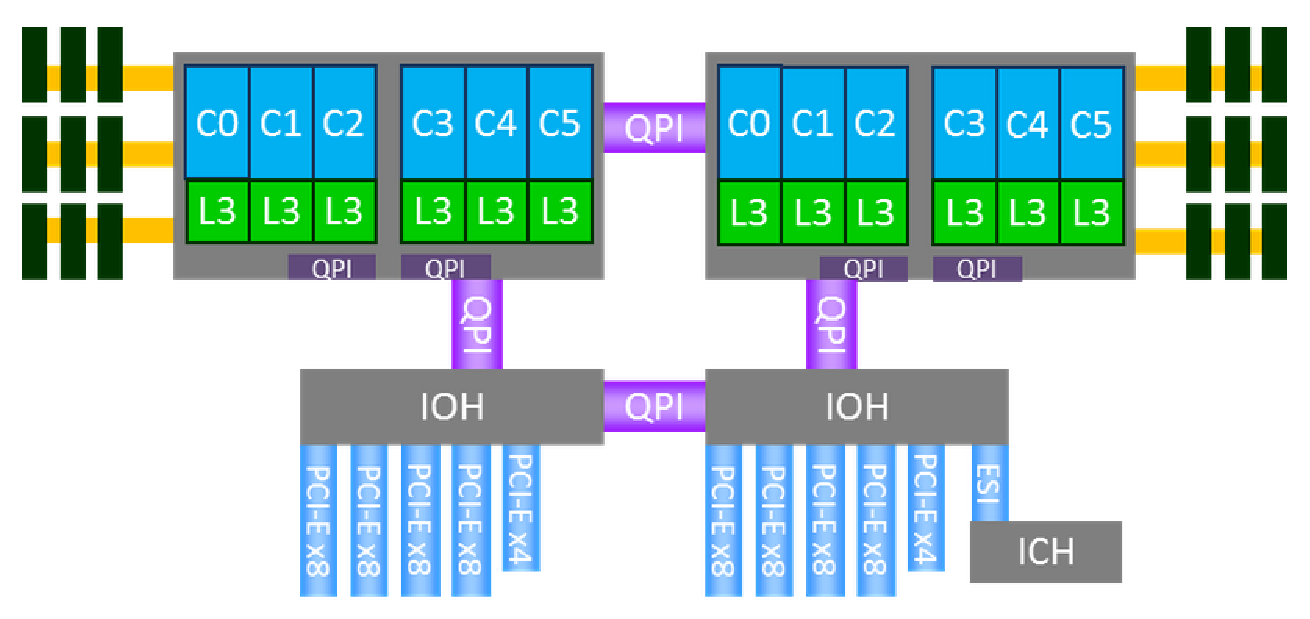
\includegraphics[height=5cm,
    angle=0]{./images/Xeon5600-Chipset5520.eps}}
\caption{Xeon 5600 (Westmere) 6-core with 2 IOH}
\label{fig:Xeon5600_Chipset5520}
\end{figure}

For best performance, depending on how many GB for memory, and whether single
processor or dual processor is used, we can choose the proper memory
configuration setting (i.e. what type of memory to buy, how many DIMMs, and how
they are plugged in).
\url{http://h20331.www2.hp.com/Hpsub/downloads/Mini_WP_Z800_memory.pdf}

To get information abount number of processors, we need to know
\begin{itemize}
  \item Physical socket : where a physical processor fits (used for licensing)
  \item Physical core: within a physical processor (multi-core)
  \item Logical core: within a physical core (hyper-threading). Depending on
  application, hyperthreading can improve performance
  5-30\%.\footnote{\url{http://www.sqlservercentral.com/blogs/glennberry/2010/10/09/what-are-physical-sockets_2C00_-physical-cores_2C00_-and-logical-cores-and-why-does-it-matter_3F00_/}}.
  With hyperthreading, we can have 2 threads/physical core. So, the number of
  logical cores = (number of threads-per-core) x (number of physical cores per
  processor) x (number of processors).
\end{itemize}
CMT = Cluster-based MultiThreading (or Clustered MultiThreading) invented by
AMD to compete with Intel Hyperthreading, which is SMT = Simultaneous
MultiThreading. The idea of hyperthreading first started with IBM since
1968\footnote{\url{http://scalibq.wordpress.com/2012/02/14/the-myth-of-cmt-cluster-based-multithreading/}}.



\subsection{HP Z820}
\label{sec:HP_Z820}

HP Z820 starts to use Intel Xeon E5-2600 series (Sandy Bridge, 32nm), with Intel
LGA2011 socket (4 memory channels per CPU, DDR3-1600 with ECC-protected), Intel
C600-series Chipset (codename Patsburg, e.g.
C602), hardware RAID 0/1/5/10 capable, PCI-E gen3. L3 cache is increaed upto
16MB from 12MB in Westmere. As shown in Fig.\ref{fig:IntelC600chipset},
connecting between 2 sockets is dual-QPI (up to 8GT/s), rather than single-QPI
in earlier chipsets. NOTE: To use Nvidia C2075 GPU, use 1125W power supply.

\begin{figure}[hbt]
  \centerline{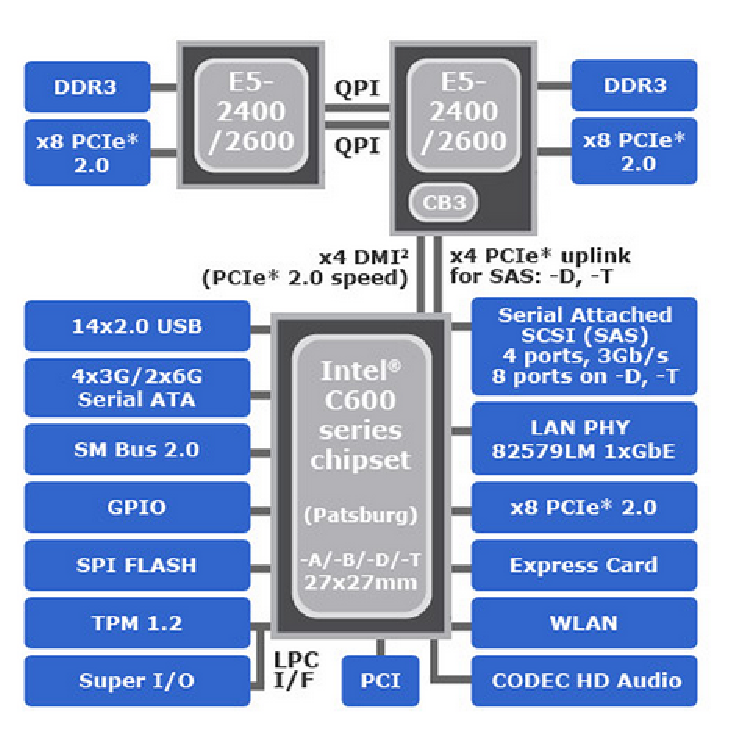
\includegraphics[height=5cm,
    angle=0]{./images/IntelC600chipset.eps}}
\caption{Intel C600 Chipset}
\label{fig:IntelC600chipset}
\end{figure}

Intel Xeon E5-2600 run as much as 2.2x faster than Xeon 5600-series. One of the
largest performance improvement is AVX, that increases vector size from 128-bit
to 256-bits, i.e. double the FP
capability\footnote{\url{http://microway.com/hpc-tech-tips/2012/04/achieve-the-best-performance-intel-xeon-e5-2600-sandy-bridge/}}.
To take advantage of the new features, Linux kernel 2.6.30 or later must be
used. QPI speed varies by processor model (6.4GT/s for basic, 7.2GT/s for
standard, and 8.0GT/s for advanced).

A single socket connects to the IOH (Intel C602 chipset), Fig.\ref{fig:HPZ820}.
Compared to HP Z800, HP Z820 is better
\begin{enumerate}
  \item more core per CPU (8-core vs. 6-core)
  \item higher memory bandwidth (51.2 GB/s Socket LGA2011 vs. 32 GB/s LGA1366)
  \item faster I/O (PCI-E Gen3 vs PCI-E Gen2)
  \item larger and faster L3 cache (16MB vs. 12MB)
  \item faster internal buses (QPI speed 8 GB/s vs. 6.4 GT/s)
  \item dual-QPI between processors
\end{enumerate}

\begin{figure}[hbt]
  \centerline{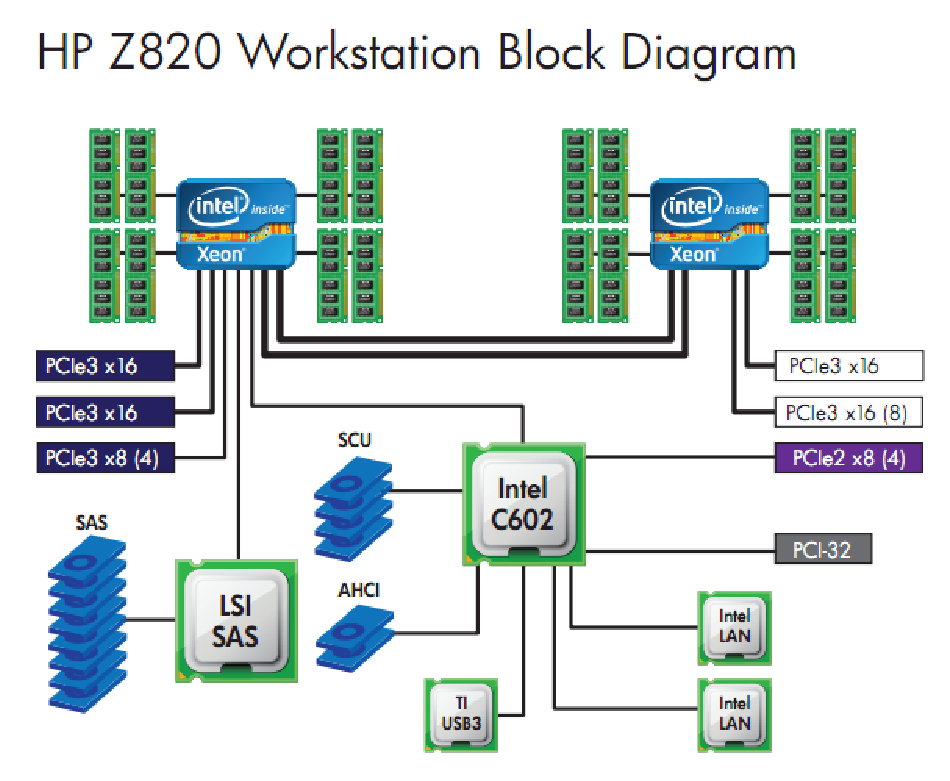
\includegraphics[height=5cm,
    angle=0]{./images/HPZ820.eps}}
\caption{HP Z820 with Intel C602 Chipset}
\label{fig:HPZ820}
\end{figure}



\subsection{BIOS setting HP Z800}
\label{sec:BIOS_Z800}

\url{http://wikihelp.autodesk.com/Flame_Premium/enu/2013/Help/Installation_Guides/01_Flame_Premium_Installation_and_Configuration_Guide/0002-Hardware2/0010-Configur10}

If you don't use Network Boot ROM, you should Disable all Option ROM Download.
For dual processors, we should enable ``Hyper-threading'' and disable Memory
Node Interleave. 

\subsubsection{NUMA memory}

In the Advanced option in BIOS setting
\begin{enumerate}
  \item {\bf NUMA split mode} can provide enhanced memory performance by
  increasing memory operation speed. It should be enabled in Windows, and
  disable for Linux. This is mutually exclusive with Memory Mode Interleaves. 
  
  On NUMA architecture with dual Intel Xeon 5500-series, a pCPU accessing memory
  on another domain is 20\% more costly than local. By using the default setting
  (i.e. Memory Mode Interleave is disabled), the system builds a System Resource
  Allocation Table (SRAT). ESX uses SRAT to understand which memory bank is
  local to a pCPU and tries to allocate data on these memory banks
  
  \item For dual socket workstations, e.g. 2 Xeon CPUs, {\bf Memory Mode
  Interleave} should be disabled (i.e. UMA is not in used). When we enable, the
  ESX will be unaware of the underlying physical architecture. When we disable,
  memory modules must be installed in the proper
  order.\footnote{\url{http://frankdenneman.nl/2010/12/node-interleaving-enable-or-disable/}}
  
  
  \item {\bf Enhanced Memory Performance}: runs DIMMS at a higher frequency on
  certain configurations and platforms.
\end{enumerate}

\subsubsection{ACPI}

ACPI is power management spec.

\subsubsection{AHCI and SATA}

AHCI specifies disk mode for SATA hard drive. SATA is a replacement for IDE
(parallel ATA). SATA uses smaller cable size (7-pin), supports hot-swapping,
faster data transfer. To communicate with SATA disk, AHCI is an open host controller
interface which has becomed the de factor standard. So, to use SATA features,
AHCI need to be enabled (installed); otherwise, it runs in IDE emulation mode.
RAID mode also has AHCI enabled. NOTE: Windows XP doesn't support AHCI, and thus
requires a properietary driver. There are different revision of SATA spec
\begin{itemize}
  \item SATA 1.0: 1.5 Gbit/sec
  \item SATA 2.0 (eSATA): 3.0 Gbit/sec
  \item SATA 3.0: 6.0 Gbit/sec	
  \item SATA 3.1: support solid-state drive, 1.8'' SATA drive, some DVD/Blue-ray
  drive $\rightarrow$ using with mini SATA (mSATA) cable.
\end{itemize}
 
Other standards: (parallel) SCSI, SAS (Serial Attached SCSI). SAS supports 3.0
Gbit/sec, then to 6 Gbit/sec (Feb, 2009), and will be 12 Gbit/sec (near
future).

\subsection{BIOS setting HP Z820}
\label{sec:BIOS_Z820}

\url{http://wikihelp.autodesk.com/Flame_Premium/enu/2013/Help/Installation_Guides/01_Flame_Premium_Installation_and_Configuration_Guide/0002-Hardware2/Configure_Z820_BIOS}

\begin{enumerate}
  \item Boot Order -- EFI Boot sources (disable)
  \item OS Power Management -- Runtime Power Management (Disable)
  \item OS Power Management -- Idle Power Saving (Normal)
  \item OS Power Management -- Turbo Mode (disable)
  \item Hardware Power Management -- SATA Power Management (Disable)
  \item Advanced -- Bus Options - Numa (disable)
  \item Advanced -- Device Options -- Internal Speaker (disable)
    
\end{enumerate}

\section{Change the current root partition from ext2 to ext3}

\url{http://www.karakas-online.de/forum/viewtopic.php?t=667}


\section{FPGA}

\subsection{SDAccel}


\subsection{Xilinx Runtime Environment}


If you install new protobuf from source - make sure you remove old packages
\begin{verbatim}
sudo apt-get purge protobuf-compiler libprotobuf-dev libprotoc-dev 
\end{verbatim}

Boost needs to be compiled with cxxstd=c++14.  If you install boost from source, make sure you remove old packages
\begin{verbatim}

sudo apt-get purge libboost-filesystem1.58-dev libboost-program-options1.58-dev \
     libboost-program-options1.58.0 libboost-system1.58-dev libboost1.58-dev

\end{verbatim}

To see all possible errors, edit build.sh and add
\begin{verbatim}
-DCMAKE_VERBOSE_MAKEFILE=ON

#into both Debug and Release lines
 time $CMAKE -DRDI_CCACHE=$ccache -DCMAKE_BUILD_TYPE=Debug -DCMAKE_EXPORT_COMPILE_COMMANDS=ON -DCMAKE_VERBOSE_MAKEFILE=ON ../../src

\end{verbatim}


FIX:
\begin{verbatim}
pip install sphinx_rtd_theme --user

# select python environment
# a mobile-friendly sphinx theme made for readthedocs.org
conda config --add channels conda-forge
conda install sphinx_rtd_theme

#conda install -c anaconda sphinx_rtd_theme 

\end{verbatim}